\documentclass{article}

\usepackage[margin=1.2cm, top=1cm, bottom=1.8cm]{geometry}
\pagestyle{plain}
\linespread{1.25}

\usepackage{fontspec}
\usepackage{unicode-math}
\usepackage[main=greek, english]{babel}

\setmainfont{CMU Serif}
\setsansfont{CMU Sans Serif}
\setmonofont{CMU Typewriter Text}
\setmathfont{Latin Modern Math}

\usepackage{amsmath, enumitem}
\usepackage{dirtytalk, caption, subcaption, array, graphicx}
\usepackage{booktabs}
\usepackage{placeins}
\usepackage{titlesec}
\usepackage{soul}
\usepackage[unicode]{hyperref}
\usepackage{verbatim}

\usepackage{pdfpages}

\usepackage{tikz}
\usetikzlibrary{arrows.meta, positioning}

\graphicspath{{../benchmarks/diagrams/}{exercises/1 st/benchmarks/diagrams/}{./}}

\hypersetup{
hidelinks,
bookmarksopen=true,
bookmarksnumbered=true,
pdftitle={Προηγμένα Θέματα Αρχιτεκτονικής Υπολογιστών - 3η Εργαστηριακή Άσκηση},
pdfauthor={Πέππας Μιχαήλ-Αθανάσιος}
}

\newcolumntype{P}[1]{>{\centering\arraybackslash}p{#1}}
\titleformat*{\subsubsection}{\large\bfseries}
\newcommand{\code}[1]{\texttt{\detokenize{#1}}}
\providecommand{\textenglish}[1]{\foreignlanguage{english}{#1}}

\begin{document}

\begin{center}
{
\Large
{
\textbf{ΕΘΝΙΚΟ ΜΕΤΣΟΒΙΟ ΠΟΛΥΤΕΧΝΕΙΟ\\
ΣΧΟΛΗ ΗΛΕΚΤΡΟΛΟΓΩΝ ΜΗΧΑΝΙΚΩΝ\\
ΚΑΙ ΜΗΧΑΝΙΚΩΝ ΥΠΟΛΟΓΙΣΤΩΝ}
}


\vspace{1.5cm}
\rule{18cm}{0.5pt}

Τομέας Τεχνολογίας, Πληροφορικής και Υπολογιστών\\
Εργαστήριο Υπολογιστικών Συστημάτων\\

\rule{18cm}{0.5pt}

\textbf{Προηγμένα Θέματα Αρχιτεκτονικής Υπολογιστών}\\
\textbf{3η Εργαστηριακή Άσκηση}\\
}


\end{center}

\vspace{0.8cm}
\begin{center}
\IfFileExists{EMP Logo.png}{\includegraphics[width=7cm]{EMP Logo.png}}{\vspace{2.5cm}}
\end{center}

\Large
{
\vspace{0.8cm}
\noindent
\textbf{Στοιχεία Φοιτητή}
\begin{itemize}
\item Όνομα: Πέππας Μιχαήλ-Αθανάσιος
\item Αριθμός Μητρώου: 03121026
\item Email: \href{mailto:el21026@mail.ntua.gr}{el21026@mail.ntua.gr}
\item Ημερομηνία Παράδοσης Αναφοράς: 26.06.2026
\end{itemize}
}

\newpage
\tableofcontents

\newpage

\section{Εισαγωγή}

Η παρούσα αναφορά πραγματεύεται την τρίτη εργαστηριακή άσκηση του μαθήματος \textit{Προηγμένα Θέματα Αρχιτεκτονικής Υπολογιστών}. Το αντικείμενο της άσκησης είναι η υλοποίηση, η εκτέλεση και η συγκριτική αξιολόγηση διαφορετικών μηχανισμών συγχρονισμού σε πολυπύρηνες αρχιτεκτονικές κοινής μνήμης. Συγκεκριμένα, μελετώνται τέσσερις υλοποιήσεις spinlock, δηλαδή οι \code{TAS_CAS}, \code{TAS_TS}, \code{TTAS_CAS} και \code{TTAS_TS}, καθώς και η υλοποίηση \code{MUTEX} της βιβλιοθήκης Pthreads, η οποία χρησιμοποιείται ως σημείο αναφοράς.

Ο βασικός στόχος δεν είναι μόνο να διαπιστωθεί ποια υλοποίηση δίνει μικρότερο χρόνο εκτέλεσης, αλλά να ερμηνευθεί η συμπεριφορά κάθε μηχανισμού συγχρονισμού σε σχέση με την αρχιτεκτονική του συστήματος. Έτσι, η αξιολόγηση γίνεται τόσο σε προσομοιωμένο σύστημα μέσω του \textenglish{Sniper Multicore Simulator}, όσο και σε πραγματικό πολυπύρηνο σύστημα. Επιπλέον, εξετάζεται η επίδραση της τοπολογίας των νημάτων, δηλαδή το πώς μεταβάλλεται η συμπεριφορά των κλειδωμάτων όταν τα νήματα μοιράζονται ή δεν μοιράζονται συγκεκριμένα επίπεδα της ιεραρχίας κρυφής μνήμης.

Η εργασία συνδέεται άμεσα με τη θεωρία του μαθήματος για τις παράλληλες αρχιτεκτονικές, τη συνάφεια κρυφών μνημών, τα μοντέλα συνέπειας μνήμης και τους μηχανισμούς συγχρονισμού. Σε ένα σύστημα κοινής μνήμης, η ύπαρξη πολλών αντιγράφων της ίδιας cache line σε διαφορετικές caches δημιουργεί την ανάγκη για πρωτόκολλα coherence, ώστε όλες οι επεξεργαστικές μονάδες να έχουν συνεπή εικόνα για τις τιμές των διαμοιραζόμενων δεδομένων. Όταν όμως ο συγχρονισμός βασίζεται σε ενεργό αναμονή και σε ατομικές λειτουργίες που μεταβάλλουν τη μεταβλητή κλειδώματος, το coherence protocol επιβαρύνεται σημαντικά, καθώς η cache line του lock μετακινείται συχνά μεταξύ καταστάσεων και πυρήνων.

Με βάση τα παραπάνω, η άσκηση εξετάζει το κλασικό πρόβλημα της κλιμάκωσης των κρίσιμων περιοχών που προστατεύονται με locks. Καθώς αυξάνεται ο αριθμός των νημάτων, αυξάνεται και ο ανταγωνισμός για την ίδια μεταβλητή κλειδώματος. Ιδανικά, ένα παράλληλο πρόγραμμα θα έπρεπε να μειώνει τον χρόνο εκτέλεσης όσο αυξάνεται το πλήθος των πυρήνων. Στην παρούσα εργασία, όμως, το κύριο φορτίο εκτέλεσης συγκεντρώνεται γύρω από μία κοινή κρίσιμη περιοχή, άρα ο συγχρονισμός μετατρέπεται σε σειριακό σημείο συμφόρησης. Επομένως, η αύξηση των νημάτων δεν αναμένεται να οδηγεί σε ιδανική επιτάχυνση. Αντιθέτως, αναμένεται να αναδείξει το κόστος του coherence traffic, των ατομικών λειτουργιών και της συμπεριφοράς υπό contention κάθε lock.

Η αναφορά οργανώνεται ως εξής. Αρχικά παρουσιάζεται το θεωρητικό υπόβαθρο της άσκησης, με έμφαση στον συγχρονισμό, στη συνάφεια κρυφών μνημών και στις διαφορές μεταξύ TAS και TTAS. Έπειτα περιγράφεται η υλοποίηση των μηχανισμών κλειδώματος και η πειραματική μεθοδολογία. Στη συνέχεια παρουσιάζονται αναλυτικά τα αποτελέσματα των προσομοιώσεων στον Sniper, τα ενεργειακά αποτελέσματα μέσω McPAT, οι μετρήσεις στο πραγματικό σύστημα και τέλος τα πειράματα τοπολογίας. Σε όλες τις περιπτώσεις παρατίθενται τόσο τα διαγράμματα όσο και οι αριθμητικοί πίνακες των αποτελεσμάτων.

\section{Θεωρητικό Υπόβαθρο}

\subsection{Παράλληλες αρχιτεκτονικές και συγχρονισμός}

Οι σύγχρονες πολυπύρηνες αρχιτεκτονικές αξιοποιούν τον παραλληλισμό σε επίπεδο νήματος, δηλαδή το \textenglish{Thread-Level Parallelism} ή TLP. Σε αντίθεση με τον παραλληλισμό επιπέδου εντολής, ο οποίος εντοπίζεται και αξιοποιείται κυρίως από τον επεξεργαστή και τον compiler, ο TLP προκύπτει ρητά από τον τρόπο με τον οποίο ο προγραμματιστής οργανώνει το πρόγραμμα σε νήματα. Όταν τα νήματα αυτά εκτελούνται σε διαφορετικούς πυρήνες και προσπελαύνουν κοινά δεδομένα, απαιτείται μηχανισμός συγχρονισμού ώστε η εκτέλεση να παραμένει ορθή.

Η ανάγκη συγχρονισμού προκύπτει όταν περισσότερα από ένα νήματα μπορούν να διαβάσουν ή να τροποποιήσουν έναν κοινό πόρο. Στην παρούσα εργασία, ο κοινός πόρος είναι η μεταβλητή \code{val}, η οποία ενημερώνεται εντός κρίσιμης περιοχής. Για να είναι ορθή η εκτέλεση, κάθε νήμα πρέπει να εισέρχεται μόνο του στην κρίσιμη περιοχή. Αν δύο νήματα εκτελέσουν ταυτόχρονα την ενημέρωση της \code{val}, το τελικό αποτέλεσμα μπορεί να είναι λανθασμένο, λόγω data race.

Η λειτουργία ενός lock βασίζεται σε δύο βασικές πράξεις:

\begin{itemize}
\item \textbf{Acquire}: το νήμα προσπαθεί να αποκτήσει το lock πριν εισέλθει στην κρίσιμη περιοχή.
\item \textbf{Release}: το νήμα απελευθερώνει το lock όταν ολοκληρώσει την κρίσιμη περιοχή.
\end{itemize}

Για να υλοποιηθεί σωστά το acquire, πρέπει η μετάβαση της μεταβλητής lock από κατάσταση \code{UNLOCKED} σε κατάσταση \code{LOCKED} να είναι ατομική. Διαφορετικά, δύο νήματα θα μπορούσαν να παρατηρήσουν ταυτόχρονα ότι το lock είναι ελεύθερο και να εισέλθουν και τα δύο στην κρίσιμη περιοχή. Γι' αυτό χρησιμοποιούνται ατομικές read-modify-write εντολές.

\subsection{Συνάφεια κρυφών μνημών και κόστος των locks}

Σε ένα πολυπύρηνο σύστημα κοινής μνήμης, κάθε πυρήνας διαθέτει ιδιωτικές ή μερικώς διαμοιραζόμενες caches. Όταν πολλά νήματα προσπελαύνουν την ίδια μεταβλητή lock, η cache line που περιέχει το lock γίνεται σημείο έντονου ανταγωνισμού. Το coherence protocol πρέπει να εξασφαλίζει ότι κάθε πυρήνας βλέπει συνεπή τιμή για το lock. Η διαδικασία αυτή, όμως, έχει κόστος: απαιτούνται invalidations, μεταφορές ownership και ανταλλαγή μηνυμάτων στο δίκτυο διασύνδεσης ή στο υποσύστημα συνοχής του συστήματος.

Στις προσομοιώσεις χρησιμοποιείται στον Sniper πρωτόκολλο \code{parametric_dram_directory_msi}. Το πρωτόκολλο MSI διακρίνει τρεις βασικές καταστάσεις για κάθε cache line:

\begin{itemize}
\item \textbf{M -- Modified}: η cache line έχει τροποποιηθεί και το συγκεκριμένο αντίγραφο είναι το μοναδικό έγκυρο.
\item \textbf{S -- Shared}: η cache line μπορεί να βρίσκεται σε περισσότερες από μία caches και είναι καθαρή.
\item \textbf{I -- Invalid}: το αντίγραφο της cache line δεν είναι έγκυρο.
\end{itemize}

Οι ατομικές λειτουργίες που γράφουν στη μεταβλητή lock απαιτούν συνήθως αποκλειστική πρόσβαση στην αντίστοιχη cache line. Επομένως, όταν πολλά νήματα εκτελούν επαναλαμβανόμενα αποτυχημένες ατομικές πράξεις στο ίδιο lock, η cache line μετακινείται διαρκώς μεταξύ πυρήνων ή προκαλεί συνεχείς invalidations. Αυτός είναι ο βασικός λόγος για τον οποίο οι απλές υλοποιήσεις TAS τείνουν να μην κλιμακώνονται αποδοτικά υπό υψηλό contention.

\subsection{TAS και TTAS}

Ο μηχανισμός \textenglish{Test-And-Set} επιχειρεί να αποκτήσει το lock εκτελώντας ατομική πράξη σε κάθε επανάληψη του βρόχου spin. Αν το lock είναι ήδη κατειλημμένο, η προσπάθεια αποτυγχάνει και το νήμα επαναλαμβάνει την ίδια ατομική πράξη. Σε αφαιρετική μορφή, η λογική του TAS είναι:

\begin{verbatim}
while atomic_exchange(lock, LOCKED) == LOCKED
\end{verbatim}

ή, αντίστοιχα, με compare-and-swap:

\begin{verbatim}
while CAS(lock, UNLOCKED, LOCKED) != UNLOCKED
\end{verbatim}

Το πλεονέκτημα του TAS είναι η απλότητα. Το μειονέκτημά του είναι ότι κάθε αποτυχημένη προσπάθεια απόκτησης είναι ατομική read-modify-write πράξη. Άρα, ακόμη και όταν το lock είναι εμφανώς κατειλημμένο, τα νήματα εξακολουθούν να προκαλούν κίνηση write-intent στη cache line του lock.

Ο μηχανισμός \textenglish{Test-And-Test-And-Set} προσπαθεί να μειώσει αυτό το πρόβλημα. Αντί να εκτελεί ατομική πράξη σε κάθε επανάληψη, πρώτα κάνει spin με απλές αναγνώσεις της τιμής του lock. Μόνο όταν παρατηρήσει ότι το lock φαίνεται ελεύθερο, επιχειρεί την ατομική πράξη:

\begin{verbatim}
while lock == LOCKED: spin with ordinary loads
then attempt CAS or test_and_set
\end{verbatim}

Με αυτόν τον τρόπο, όσο το lock παραμένει κατειλημμένο, τα νήματα που περιμένουν εκτελούν κυρίως απλές αναγνώσεις. Η cache line μπορεί να βρίσκεται σε κατάσταση Shared σε περισσότερες caches, χωρίς να προκαλείται συνεχώς invalidation. Ατομική εγγραφή εμφανίζεται μόνο όταν κάποιο νήμα επιχειρεί πράγματι να αποκτήσει το lock. Επομένως, θεωρητικά, οι υλοποιήσεις TTAS αναμένεται να έχουν καλύτερη συμπεριφορά από τις υλοποιήσεις TAS όταν υπάρχει έντονος ανταγωνισμός.

\subsection{Pthread mutex ως σημείο αναφοράς}

Η υλοποίηση \code{MUTEX} βασίζεται στο \code{pthread_mutex_t}. Σε αντίθεση με τα απλά spinlocks, ένα mutex της βιβλιοθήκης Pthreads μπορεί να έχει διαφορετική συμπεριφορά, καθώς η υλοποίηση του runtime και του λειτουργικού συστήματος μπορεί να επιλέξει blocking, scheduling ή πιο σύνθετες πολιτικές αναμονής ανάλογα με την περίπτωση. Γι' αυτό, το \code{MUTEX} δεν συγκρίνεται μόνο ως ένας ακόμη μηχανισμός αμοιβαίου αποκλεισμού, αλλά και ως ένας μηχανισμός που αντιπροσωπεύει τη συμπεριφορά μιας βελτιστοποιημένης βιβλιοθήκης συστήματος.

Στον Sniper, η σύγκριση με το \code{MUTEX} δείχνει πώς μοντελοποιείται ένας τυπικός μηχανισμός συγχρονισμού του συστήματος μέσα στο προσομοιωμένο περιβάλλον. Στο πραγματικό σύστημα, η σύγκριση επηρεάζεται επιπλέον από τον scheduler, από τη συγκεκριμένη υλοποίηση της βιβλιοθήκης Pthreads, από την τοπολογία του επεξεργαστή και από τις δυναμικές πολιτικές συχνότητας και ισχύος του laptop.

\subsection{Μετρικές απόδοσης και ενέργειας}

Η κύρια μετρική απόδοσης στις προσομοιώσεις είναι οι κύκλοι εκτέλεσης της περιοχής ενδιαφέροντος, δηλαδή του \textenglish{Region of Interest} ή ROI. Η μέτρηση αρχίζει αφού όλα τα νήματα έχουν δημιουργηθεί και συγχρονιστεί, ώστε να μην περιλαμβάνεται το κόστος δημιουργίας των threads, και ολοκληρώνεται αφού όλα τα νήματα έχουν ολοκληρώσει τις επαναλήψεις τους.

Πέρα από τον χρόνο εκτέλεσης, χρησιμοποιούνται ενεργειακές μετρικές από το McPAT. Η συνολική ενέργεια από μόνη της δεν αρκεί πάντα για πλήρη αξιολόγηση, επειδή μια υλοποίηση μπορεί να καταναλώνει λιγότερη ισχύ αλλά να εκτελείται πολύ πιο αργά. Γι' αυτό χρησιμοποιούνται επίσης τα \textenglish{Energy-Delay Product} και \textenglish{Energy-Delay Squared Product}:

\[
EDP = \mathrm{Energy} \cdot \mathrm{Runtime}
\]

\[
ED^2P = \mathrm{Energy} \cdot \mathrm{Runtime}^2
\]

Το $EDP$ συνδυάζει ενέργεια και χρόνο εκτέλεσης με ίσο βάρος, ενώ το $ED^2P$ δίνει μεγαλύτερη βαρύτητα στον χρόνο εκτέλεσης. Στην παρούσα εργασία οι μετρικές αυτές είναι ιδιαίτερα χρήσιμες, επειδή κάποιες υλοποιήσεις εμφανίζουν υψηλή στιγμιαία ισχύ λόγω έντονων ατομικών πράξεων, ενώ άλλες εκτελούνται για μεγαλύτερο χρονικό διάστημα.

\section{Υλοποίηση}

\subsection{Γενική δομή του προγράμματος}

Το πρόγραμμα της άσκησης βασίζεται στο αρχείο \code{locks_scalability.c}. Η εκτέλεση δέχεται τρεις παραμέτρους γραμμής εντολών:

\begin{itemize}
\item \code{nthreads}: αριθμός νημάτων που δημιουργούνται.
\item \code{iterations}: αριθμός επαναλήψεων της κρίσιμης περιοχής ανά νήμα.
\item \code{grain}: μέγεθος του τεχνητού υπολογιστικού φορτίου εντός της κρίσιμης περιοχής.
\end{itemize}

Κάθε νήμα εκτελεί την ίδια συνάρτηση \code{thread_fn}. Αρχικά τοποθετείται σε συγκεκριμένη CPU μέσω affinity, στη συνέχεια συγχρονίζεται με τα υπόλοιπα νήματα μέσω barrier και έπειτα εισέρχεται στον κύριο βρόχο. Σε κάθε επανάληψη αποκτά το lock, εκτελεί την εργασία της κρίσιμης περιοχής, ενημερώνει τη διαμοιραζόμενη μεταβλητή \code{val} και απελευθερώνει το lock.

Η παράμετρος \code{grain} καθορίζει το πλήθος των εσωτερικών τεχνητών πράξεων:

\[
x \leftarrow x \cdot 2.0,\qquad x \leftarrow x / 2.0
\]

Επομένως, η αύξηση της τιμής grain αυξάνει τη διάρκεια της κρίσιμης περιοχής. Αυτό είναι σημαντικό πειραματικά, επειδή αλλάζει τη σχετική σημασία του κόστους συγχρονισμού ως προς το κόστος χρήσιμης εργασίας. Για μικρή τιμή grain, το κόστος συγχρονισμού κυριαρχεί. Για μεγαλύτερη τιμή grain, το lock παραμένει δεσμευμένο για περισσότερο χρόνο, αλλά το κόστος της ατομικής απόκτησης επιμερίζεται σε μεγαλύτερη ποσότητα υπολογισμού.

\subsection{Υλοποιημένες εκδόσεις κλειδώματος}

Οι υλοποιήσεις βρίσκονται στο αρχείο \code{lock.h}. Η μεταβλητή κλειδώματος ορίζεται ως:

\[
\code{typedef volatile int spinlock_t;}
\]

με σταθερές:

\[
\code{UNLOCKED} = 0,\qquad \code{LOCKED} = 1
\]

Υλοποιήθηκαν οι τέσσερις ζητούμενες εκδόσεις spinlock, δύο με compare-and-swap και δύο με test-and-set. Ο Πίνακας~\ref{tab:lock-implementations} συνοψίζει τη λογική κάθε υλοποίησης.

\begin{table}[htbp]
\centering
\small
\caption{Υλοποιήσεις μηχανισμών κλειδώματος.}
\label{tab:lock-implementations}
\begin{tabular}{P{2.7cm} P{4.4cm} P{7.7cm}}
\toprule
\textbf{Υλοποίηση} & \textbf{Atomic primitive} & \textbf{Λογική acquire} \\
\midrule
\code{TAS_CAS} &
\code{__sync_val_compare_and_swap} &
Επαναλαμβάνει ατομικό compare-and-swap από \code{UNLOCKED} σε \code{LOCKED} μέχρι να πετύχει. \\
\midrule
\code{TAS_TS} &
\code{__sync_lock_test_and_set} &
Επαναλαμβάνει ατομικό test-and-set, γράφοντας \code{LOCKED} και ελέγχοντας την προηγούμενη τιμή. \\
\midrule
\code{TTAS_CAS} &
\code{__sync_val_compare_and_swap} &
Πρώτα κάνει spin με απλές αναγνώσεις όσο το lock είναι \code{LOCKED}. Έπειτα επιχειρεί CAS μόνο όταν το lock φανεί ελεύθερο. \\
\midrule
\code{TTAS_TS} &
\code{__sync_lock_test_and_set} &
Πρώτα κάνει spin με απλές αναγνώσεις. Έπειτα επιχειρεί test-and-set μόνο όταν παρατηρήσει \code{UNLOCKED}. \\
\midrule
\code{MUTEX} &
mutex της Pthreads &
Χρησιμοποιεί τις κλήσεις \code{pthread_mutex_lock} και \code{pthread_mutex_unlock}. \\
\bottomrule
\end{tabular}
\end{table}

Η απελευθέρωση των spinlocks γίνεται με:

\[
\code{__sync_lock_release}
\]

Η χρήση του συγκεκριμένου intrinsic είναι σημαντική, επειδή δεν πρόκειται απλώς για μια απλή ανάθεση μηδενισμού. Η λειτουργία release έχει την κατάλληλη σημασιολογία μνήμης ώστε οι εγγραφές που έγιναν μέσα στην κρίσιμη περιοχή να γίνουν ορατές πριν το lock εμφανιστεί ως ελεύθερο σε άλλο νήμα.

\subsection{Έλεγχος ορθότητας}

Για να επιβεβαιωθεί ότι οι μηχανισμοί συγχρονισμού εξασφαλίζουν πράγματι αμοιβαίο αποκλεισμό, προστέθηκε έλεγχος ορθότητας στο πρόγραμμα. Κάθε εκτέλεση ελέγχει ότι η τελική τιμή της μεταβλητής \code{val} ισούται με:

\[
\text{\texttt{val}} = \text{\texttt{nthreads}} \cdot \text{\texttt{iterations}}
\]

Ο έλεγχος αυτός είναι επαρκής για τη συγκεκριμένη δομή του benchmark, επειδή κάθε είσοδος στην κρίσιμη περιοχή αυξάνει τη \code{val} κατά 1. Άρα, εάν χαθεί έστω και μία ενημέρωση λόγω ταυτόχρονης πρόσβασης, η τελική τιμή θα είναι μικρότερη από την αναμενόμενη.

Στις εκτελέσεις Sniper, ο έλεγχος γίνεται πριν από το \code{SimRoiEnd()}, ώστε το μήνυμα \code{Validation: PASS} να εμφανίζεται στα αποθηκευμένα αποτελέσματα της προσομοίωσης. Στις πραγματικές εκτελέσεις, ο έλεγχος γίνεται μετά το \code{join} όλων των νημάτων. Όλες οι τελικές εκτελέσεις που χρησιμοποιούνται στην αναφορά ολοκληρώθηκαν με επιτυχή έλεγχο ορθότητας.

\subsection{Μεταγλώττιση}

Το \code{Makefile} παράγει ξεχωριστά εκτελέσιμα για πραγματικό σύστημα και για Sniper. Για κάθε υλοποίηση δημιουργείται μία έκδοση \code{REAL} και μία έκδοση \code{SNIPER}. Οι βασικές επιλογές μεταγλώττισης δίνονται στον Πίνακα~\ref{tab:compile-flags}.

\begin{table}[htbp]
\centering
\small
\caption{Compile-time flags της υλοποίησης.}
\label{tab:compile-flags}
\begin{tabular}{P{4cm} P{10.8cm}}
\toprule
\textbf{Flag} & \textbf{Σκοπός} \\
\midrule
\code{-DREAL} & Ενεργοποιεί την εκτέλεση σε πραγματικό σύστημα και τη μέτρηση χρόνου με \code{gettimeofday}. \\
\midrule
\code{-DSNIPER} & Ενεργοποιεί τα \code{SimRoiStart()} και \code{SimRoiEnd()} για μέτρηση περιοχής ενδιαφέροντος στον Sniper. \\
\midrule
\code{-DTAS_CAS} & Μεταγλωττίζει την έκδοση TAS με compare-and-swap. \\
\midrule
\code{-DTAS_TS} & Μεταγλωττίζει την έκδοση TAS με test-and-set. \\
\midrule
\code{-DTTAS_CAS} & Μεταγλωττίζει την έκδοση TTAS με compare-and-swap. \\
\midrule
\code{-DTTAS_TS} & Μεταγλωττίζει την έκδοση TTAS με test-and-set. \\
\midrule
\code{-DMUTEX} & Μεταγλωττίζει την έκδοση με mutex της Pthreads. \\
\bottomrule
\end{tabular}
\end{table}

Τα παραγόμενα εκτελέσιμα ακολουθούν τη μορφή:

\[
\code{bin/locks_<implementation>_real}
\]

και:

\[
\code{bin/locks_<implementation>_sniper}
\]

Με αυτόν τον τρόπο αποφεύγεται η χειροκίνητη αλλαγή των flags μεταγλώττισης μεταξύ εκτελέσεων και μειώνεται η πιθανότητα πειραματικού σφάλματος.

\section{Πειραματική Μεθοδολογία}

\subsection{Περιβάλλον Sniper}

Οι προσομοιώσεις εκτελέστηκαν με Sniper 8.0 μέσω Docker. Χρησιμοποιήθηκε τοπική εικόνα \code{advca-sniper:8.0}, βασισμένη στην εικόνα του Sniper που δίνεται για την άσκηση. Για αναπαραγωγιμότητα, η βάση της εικόνας είχε σταθερό digest:

\[
\code{sha256:4f10d4bbfee057e27a52fc0dc33087813feb504bbbfff22902984e356576eaed}
\]

Επειδή η εικόνα βασίζεται σε CentOS 6, στο περιβάλλον WSL απαιτήθηκε ενεργοποίηση \code{vsyscall=emulate}. Η ιδιαιτερότητα αυτή αφορά τη συμβατότητα του παλαιότερου περιβάλλοντος χρήστη της εικόνας με νεότερους WSL kernels και δεν επηρεάζει τη λογική των πειραμάτων.

Η παραμετροποίηση του προσομοιωμένου συστήματος έγινε με το αρχείο \code{ask3.cfg}, όπως ζητείται στην εκφώνηση. Ο Πίνακας~\ref{tab:sniper-config} συνοψίζει τις βασικές παραμέτρους που χρησιμοποιήθηκαν.

\begin{table}[htbp]
\centering
\small
\caption{Βασικές παράμετροι του \code{ask3.cfg}.}
\label{tab:sniper-config}
\begin{tabular}{P{5cm} P{9.7cm}}
\toprule
\textbf{Παράμετρος} & \textbf{Τιμή} \\
\midrule
Μοντέλο πυρήνα & \code{interval}, \code{nehalem} \\
\midrule
Συχνότητα πυρήνα & \(2.66\,\text{GHz}\) \\
\midrule
Πρωτόκολλο coherence & \code{parametric_dram_directory_msi} \\
\midrule
L1 instruction cache & \(32\,\mathrm{KB}\), 8-way, \(64\,\mathrm{B}\) cache block \\
\midrule
L1 data cache & \(32\,\mathrm{KB}\), 8-way, \(64\,\mathrm{B}\) cache block \\
\midrule
L2 cache & \(1024\,\mathrm{KB}\), 8-way, \(64\,\mathrm{B}\) cache block \\
\midrule
L3 cache & \(8192\,\mathrm{KB}\), 16-way, \(64\,\mathrm{B}\) cache block \\
\midrule
Branch predictor & \code{pentium_m}, penalty 17 cycles \\
\midrule
Power model & \(45\,\mathrm{nm}\), \(V_{dd}=1.2\,\mathrm{V}\) \\
\bottomrule
\end{tabular}
\end{table}

Για κάθε προσομοίωση αποθηκεύτηκαν τα πλήρη αποτελέσματα του Sniper, μεταξύ των οποίων τα \code{sim.out}, \code{sim.cfg}, \code{sim.info}, \code{sim.stats.sqlite3}, καθώς και τα αντίστοιχα αρχεία εξόδου του McPAT. Η εξαγωγή των τελικών πινάκων έγινε από τα συγκεντρωτικά αρχεία \code{summary.csv}.

\subsection{Περιοχή ενδιαφέροντος}

Η μέτρηση στον Sniper περιορίστηκε αποκλειστικά στην κύρια περιοχή εκτέλεσης του benchmark. Τα νήματα δημιουργούνται πρώτα και συγχρονίζονται με barrier. Έπειτα το νήμα 0 καλεί:

\[
\code{SimRoiStart()}
\]

Αφού όλα τα νήματα ολοκληρώσουν τις επαναλήψεις τους, συγχρονίζονται ξανά με barrier και το νήμα 0 εκτελεί τον έλεγχο ορθότητας και έπειτα καλεί:

\[
\code{SimRoiEnd()}
\]

Η επιλογή αυτή είναι αναγκαία ώστε οι μετρήσεις να αφορούν το κόστος συγχρονισμού και την εκτέλεση της κρίσιμης περιοχής, όχι το κόστος δημιουργίας των Pthreads ή την αρχικοποίηση του προγράμματος.

\subsection{Πειράματα κλιμάκωσης στον Sniper}

Για την ενότητα κλιμάκωσης εκτελέστηκαν όλες οι ζητούμενες προσομοιώσεις για:

\[
\text{\texttt{nthreads}} \in \{1,2,4,8,16\}
\]

\[
\text{\texttt{grain}} \in \{1,10,100\}
\]

και για τις πέντε υλοποιήσεις:

\[
{\code{TAS_CAS}, \code{TAS_TS}, \code{TTAS_CAS}, \code{TTAS_TS}, \code{MUTEX}}
\]

Ο αριθμός επαναλήψεων στον Sniper ήταν:

\[
\code{iterations} = 1000
\]

Συνολικά, η μήτρα πειραμάτων της ενότητας 4.1 στον Sniper περιλαμβάνει:

\[
5 \cdot 5 \cdot 3 = 75
\]

προσομοιώσεις, οι οποίες ολοκληρώθηκαν όλες επιτυχώς.

Οι τιμές διαμοιρασμού των caches επιλέχθηκαν σύμφωνα με τα συστήματα της εκφώνησης. Για κάθε αριθμό νημάτων, ο αριθμός πυρήνων του Sniper ήταν ίσος με τον αριθμό νημάτων. Ο Πίνακας~\ref{tab:sniper-scaling-topologies} δείχνει τις τιμές \code{shared_cores} που χρησιμοποιήθηκαν.

\begin{table}[htbp]
\centering
\small
\caption{Τοπολογίες διαμοιρασμού cache στα πειράματα κλιμάκωσης Sniper.}
\label{tab:sniper-scaling-topologies}
\begin{tabular}{P{3cm} P{4cm} P{4cm} P{4cm}}
\toprule
\textbf{Νήματα / Πυρήνες} & \textbf{L2 shared cores} & \textbf{L3 shared cores} & \textbf{Σχόλιο} \\
\midrule
1 & 1 & 1 & Μονοπύρηνη εκτέλεση. \\
\midrule
2 & 2 & 2 & Κοινή L2 και L3 για τους δύο πυρήνες. \\
\midrule
4 & 4 & 4 & Όλοι οι πυρήνες κάτω από κοινή L2 και L3. \\
\midrule
8 & 4 & 8 & Δύο ομάδες L2, κοινή L3. \\
\midrule
16 & 1 & 8 & Ιδιωτικές L2, κοινή L3 ανά οκτώ πυρήνες. \\
\bottomrule
\end{tabular}
\end{table}

\subsection{Πειράματα στο πραγματικό σύστημα}

Εκτός από τις προσομοιώσεις, εκτελέστηκε το ίδιο σύνολο πειραμάτων και σε πραγματικό μηχάνημα. Το πραγματικό σύστημα ήταν laptop με επεξεργαστή \textenglish{13th Gen Intel Core i7-13700HX}. Το περιβάλλον WSL εμφάνιζε 24 λογικές CPUs, οι οποίες αντιστοιχούν σε 16 φυσικούς πυρήνες: 8 πυρήνες με SMT με δύο λογικές CPUs ο καθένας και 8 μονονηματικοί πυρήνες.

Αντί να γίνει απλή αντιστοίχιση των threads στις λογικές CPUs (0,\ldots,15), χρησιμοποιήθηκε ρητό affinity μέσω της μεταβλητής περιβάλλοντος \code{LOCKS_CPU_LIST}. Το script ανέκτησε την τοπολογία από το \code{lscpu}, ομαδοποίησε τις λογικές CPUs ανά φυσικό πυρήνα και επέλεξε έναν εκπρόσωπο από κάθε φυσικό πυρήνα. Έτσι, περιορίστηκε η πιθανότητα να τοποθετηθούν δύο νήματα λογισμικού στον ίδιο φυσικό πυρήνα ενώ υπάρχουν ακόμη διαθέσιμοι φυσικοί πυρήνες.

Οι εκπρόσωποι φυσικών πυρήνων που χρησιμοποιήθηκαν ήταν:

\[
0,2,4,6,8,10,12,14,16,17,18,19,20,21,22,23
\]

Η αντιστοίχιση των λογικών CPUs φαίνεται στον Πίνακα~\ref{tab:real-topology}.

\begin{table}[htbp]
\centering
\small
\caption{Τοπολογία λογικών CPUs του πραγματικού συστήματος.}
\label{tab:real-topology}
\begin{tabular}{P{2.2cm} P{3.8cm} P{2.2cm} P{3.8cm}}
\toprule
\textbf{Φυσικός πυρήνας} & \textbf{Logical CPUs} & \textbf{Φυσικός πυρήνας} & \textbf{Logical CPUs} \\
\midrule
0 & 0, 1 & 8 & 16 \\
1 & 2, 3 & 9 & 17 \\
2 & 4, 5 & 10 & 18 \\
3 & 6, 7 & 11 & 19 \\
4 & 8, 9 & 12 & 20 \\
5 & 10, 11 & 13 & 21 \\
6 & 12, 13 & 14 & 22 \\
7 & 14, 15 & 15 & 23 \\
\bottomrule
\end{tabular}
\end{table}

\begin{figure}[htbp]
\centering
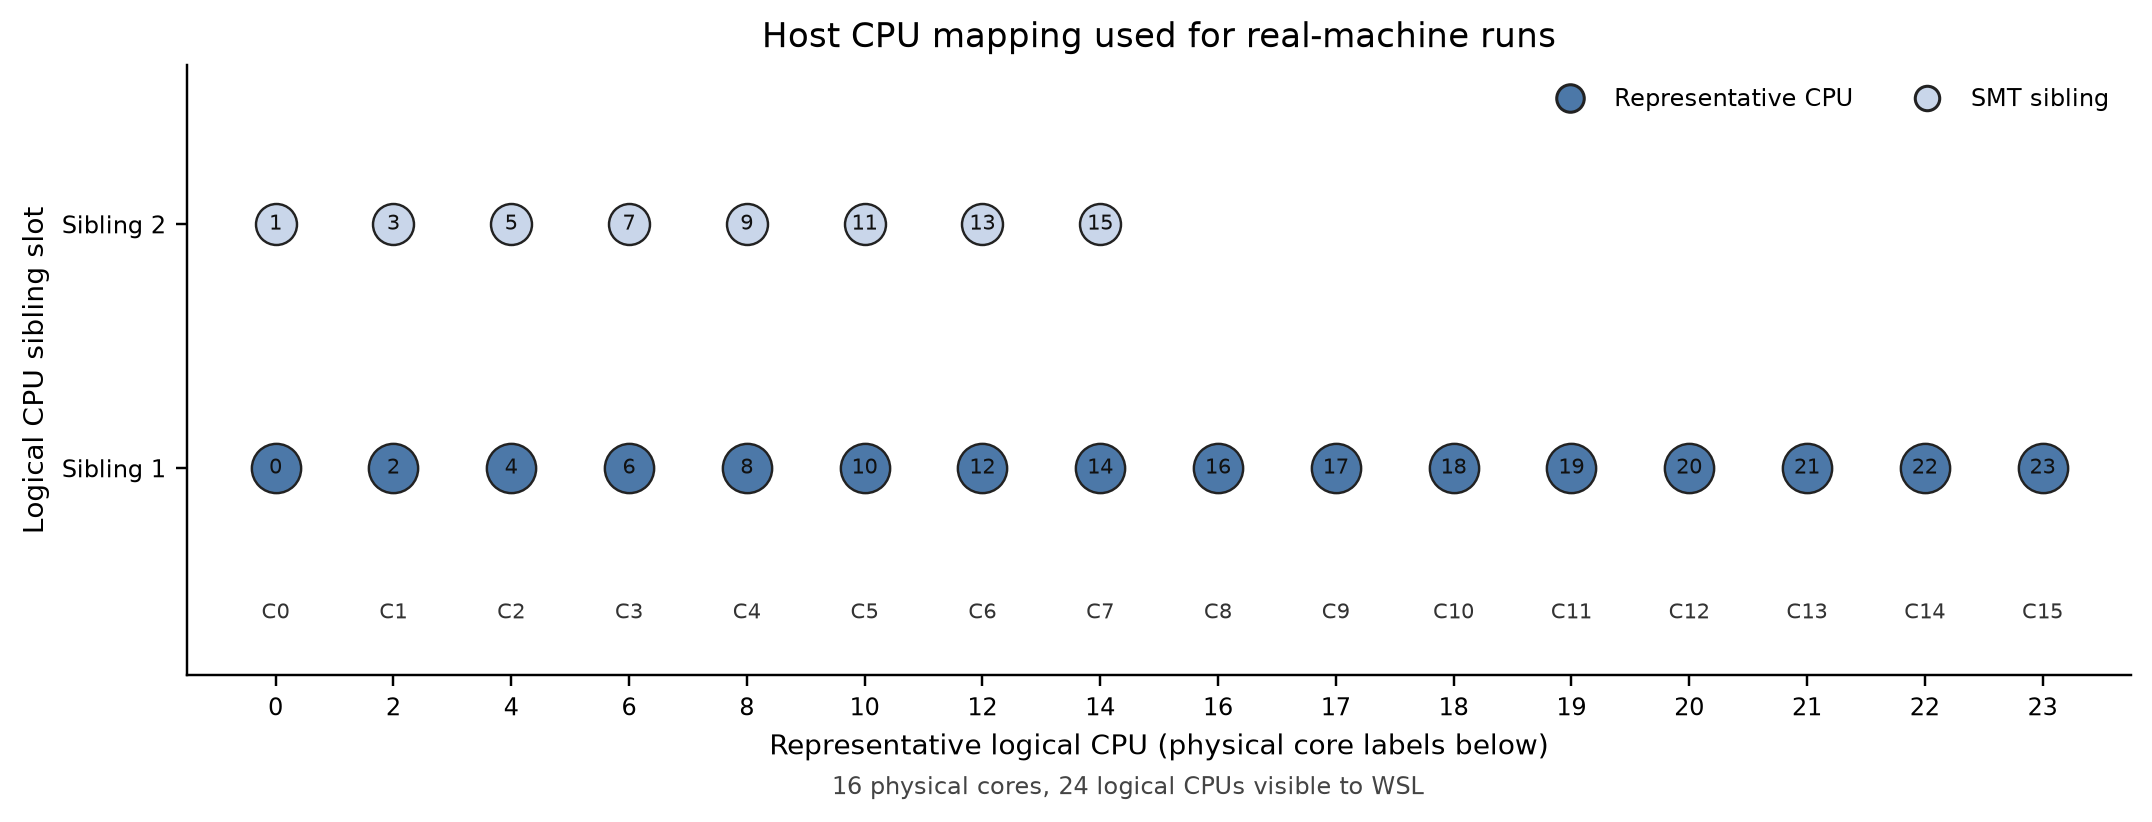
\includegraphics[width=0.78\textwidth]{host_cpu_physical_core_mapping.png}
\caption{Αντιστοίχιση φυσικών πυρήνων και λογικών CPUs στο πραγματικό σύστημα.}
\label{fig:host-cpu-mapping}
\end{figure}

Για τις πραγματικές εκτελέσεις χρησιμοποιήθηκαν τα ίδια πλήθη νημάτων και τιμές grain με τον Sniper:

\[
\text{\texttt{nthreads}} \in \{1,2,4,8,16\}
\]

\[
\text{\texttt{grain}} \in \{1,10,100\}
\]

Για κάθε συνδυασμό εκτελέστηκαν 5 επαναλήψεις και αναφέρεται κυρίως η διάμεσος τιμή. Συνολικά, το σύνολο των πειραματικών συνδυασμών στο πραγματικό σύστημα περιλαμβάνει:

\[
5 \cdot 5 \cdot 3 = 75
\]

περιπτώσεις και:

\[
75 \cdot 5 = 375
\]

μεμονωμένες εκτελέσεις.

Ο αριθμός επαναλήψεων για το πραγματικό σύστημα ορίστηκε σε:

\[
\code{iterations} = 50{,}000{,}000
\]

Η εκφώνηση ζητά ο αριθμός επαναλήψεων να είναι αρκετά μεγάλος ώστε οι χρόνοι να μπορούν να μετρηθούν με ακρίβεια, ενδεικτικά με τις εκτελέσεις ενός νήματος να είναι της τάξης μερικών δευτερολέπτων. Στην τελική εκτέλεση επιλέχθηκαν \(50{,}000{,}000\) επαναλήψεις ως πρακτικός συμβιβασμός. Μεγαλύτερες τιμές βαθμονόμησης, όπως \(150\,\mathrm{M}\) ή \(200\,\mathrm{M}\), έκαναν ορισμένες περιπτώσεις με πολλά νήματα και μεγάλο grain εξαιρετικά χρονοβόρες, με επιμέρους επαναλήψεις να διαρκούν πολλά λεπτά και το πλήρες σύνολο πειραμάτων να κινδυνεύει να απαιτήσει αρκετές επιπλέον ημέρες εκτέλεσης. Επιπλέον, το σύστημα είχε ήδη χρησιμοποιηθεί εντατικά για προηγούμενα φορτία εργασίας της άσκησης. Γι' αυτό, προτιμήθηκε να διατηρηθεί ένα πλήρες και συνεπές σύνολο πειραμάτων, με 5 επαναλήψεις ανά περίπτωση, αντί να αυξηθούν περαιτέρω οι επαναλήψεις εις βάρος της ολοκλήρωσης.

Το παραπάνω αποτελεί πειραματικό περιορισμό που πρέπει να ληφθεί υπόψη στην ερμηνεία. Οι μόνες περιπτώσεις με διάμεσο χρόνο κάτω από 1 s είναι οι εκτελέσεις ενός νήματος με \code{grain=1}, όπως φαίνεται στον Πίνακα~\ref{tab:subsecond-real}.

\begin{table}[htbp]
\centering
\small
\caption{Πραγματικές εκτελέσεις με διάμεσο χρόνο κάτω από 1 s.}
\label{tab:subsecond-real}
\begin{tabular}{P{3cm} P{2cm} P{2cm} P{3cm} P{3cm} P{3cm}}
\toprule
\textbf{Υλοποίηση} & \textbf{Νήματα} & \textbf{Grain} & \textbf{Διάμεσος (s)} & \textbf{Ελάχιστο (s)} & \textbf{Μέγιστο (s)} \\
\midrule
\code{MUTEX} & 1 & 1 & 0.625282 & 0.619223 & 0.631213 \\
\code{TAS_CAS} & 1 & 1 & 0.388580 & 0.386149 & 0.393923 \\
\code{TAS_TS} & 1 & 1 & 0.365641 & 0.363519 & 0.367187 \\
\code{TTAS_CAS} & 1 & 1 & 0.387483 & 0.384452 & 0.394591 \\
\code{TTAS_TS} & 1 & 1 & 0.365560 & 0.362871 & 0.369583 \\
\bottomrule
\end{tabular}
\end{table}

Όλες οι υπόλοιπες περιπτώσεις έχουν διάμεσο χρόνο μεγαλύτερο ή ίσο με 1 s. Στις μεμονωμένες επαναλήψεις υπήρχαν 27 από τις 375 μετρήσεις κάτω από 1 s: οι 25 αντιστοιχούν σε όλες τις επαναλήψεις των πέντε περιπτώσεων \code{threads=1, grain=1}, ενώ δύο επιπλέον επαναλήψεις με \code{threads=1, grain=10} ήταν οριακά κάτω από 1 s. Ωστόσο, οι διάμεσοι χρόνοι αυτών των \code{grain=10} περιπτώσεων ήταν πάνω από 1 s, οπότε δεν επηρεάζουν ουσιαστικά τη συγκριτική ανάλυση.

\subsection{Πειράματα τοπολογίας στον Sniper}

Στην ενότητα 4.2 εξετάστηκε η επίδραση της τοπολογίας των νημάτων. Σε όλα τα πειράματα χρησιμοποιήθηκαν:

\[
\code{nthreads}=4,\qquad \code{iterations}=1000,\qquad \code{grain}=1
\]

Οι πέντε υλοποιήσεις εκτελέστηκαν στις τρεις τοπολογίες του Πίνακα~\ref{tab:topology-experiments}. Συνολικά εκτελέστηκαν:

\[
5 \cdot 3 = 15
\]

προσομοιώσεις.

\begin{table}[htbp]
\centering
\small
\caption{Τοπολογίες πειραμάτων ενότητας 4.2.}
\label{tab:topology-experiments}
\begin{tabular}{P{3.6cm} P{3cm} P{3cm} P{6cm}}
\toprule
\textbf{Τοπολογία} & \textbf{L2 shared cores} & \textbf{L3 shared cores} & \textbf{Ερμηνεία} \\
\midrule
\code{share-all} & 4 & 4 & Τα 4 νήματα βρίσκονται κάτω από κοινή L2 και κοινή L3. \\
\midrule
\code{share-l3} & 1 & 4 & Κάθε πυρήνας έχει ιδιωτική L2, αλλά όλοι μοιράζονται κοινή L3. \\
\midrule
\code{share-nothing} & 1 & 1 & Οι πυρήνες δεν μοιράζονται ούτε L2 ούτε L3. \\
\bottomrule
\end{tabular}
\end{table}

Η αναμενόμενη επίδραση της τοπολογίας σχετίζεται με τη θέση στην οποία γίνεται η ανταλλαγή της cache line του lock. Όταν τα νήματα μοιράζονται χαμηλότερο επίπεδο cache, η επικοινωνία για τη μεταβλητή συγχρονισμού μπορεί να είναι ταχύτερη, αλλά υπάρχει και μεγαλύτερος ανταγωνισμός για τους ίδιους πόρους της cache. Όταν τα νήματα δεν μοιράζονται L2 ή L3, οι ανταλλαγές ownership γίνονται ακριβότερες, επειδή απαιτούνται περισσότερα coherence messages και μεγαλύτερη απόσταση στην ιεραρχία μνήμης. Η τελική συμπεριφορά εξαρτάται από τον μηχανισμό lock, επειδή κάθε υλοποίηση παράγει διαφορετικό μοτίβο αναγνώσεων και εγγραφών στη cache line του lock.

\subsection{Συνοπτική εικόνα πειραμάτων}

Ο Πίνακας~\ref{tab:experiment-summary} συνοψίζει όλες τις τελικές πειραματικές μήτρες που χρησιμοποιούνται στην αναφορά.

\begin{table}[htbp]
\centering
\small
\caption{Συνοπτική εικόνα τελικών πειραμάτων.}
\label{tab:experiment-summary}
\resizebox{\textwidth}{!}{
\begin{tabular}{P{3.3cm} P{2.2cm} P{4.2cm} P{3.2cm} P{2.2cm} P{2.6cm} P{2.5cm}}
\toprule
\textbf{Πείραμα} & \textbf{Πλήθος runs} & \textbf{Υλοποιήσεις} & \textbf{Νήματα} & \textbf{Iterations} & \textbf{Grain sizes} & \textbf{Επαναλήψεις} \\
\midrule
4.1 κλιμάκωση στον Sniper & 75 &
\code{TAS_CAS}, \code{TAS_TS}, \code{TTAS_CAS}, \code{TTAS_TS}, \code{MUTEX} &
1, 2, 4, 8, 16 & 1000 & 1, 10, 100 & 1 \\
\midrule
4.1 Κλιμάκωση στο πραγματικό σύστημα & 75 περιπτώσεις / 375 μεμονωμένες εκτελέσεις &
\code{TAS_CAS}, \code{TAS_TS}, \code{TTAS_CAS}, \code{TTAS_TS}, \code{MUTEX} &
1, 2, 4, 8, 16 & 50,000,000 & 1, 10, 100 & 5 \\
\midrule
4.2 τοπολογία στον Sniper & 15 &
\code{TAS_CAS}, \code{TAS_TS}, \code{TTAS_CAS}, \code{TTAS_TS}, \code{MUTEX} &
4 & 1000 & 1 & 1 \\
\bottomrule
\end{tabular}
}
\end{table}

\FloatBarrier

\section{Αποτελέσματα Κλιμάκωσης στον Sniper}

\subsection{Συνολική εικόνα των προσομοιώσεων}

Στην ενότητα αυτή παρουσιάζονται τα αποτελέσματα της ενότητας 4.1 για το προσομοιωμένο σύστημα του Sniper. Για κάθε υλοποίηση lock εκτελέστηκαν προσομοιώσεις με 1, 2, 4, 8 και 16 νήματα, για τρία διαφορετικά μεγέθη κρίσιμης περιοχής:

\[
\text{\texttt{grain}} \in \{1,10,100\}
\]

Η κύρια μετρική απόδοσης είναι το πλήθος κύκλων εκτέλεσης του ROI. Παράλληλα, μέσω McPAT εξήχθησαν η ισχύς, η ενέργεια, τα $EDP$ και $ED^2P$. Οι τιμές χρόνου εκτέλεσης των πινάκων προκύπτουν από τους κύκλους και τη συχνότητα του προσομοιωμένου πυρήνα, δηλαδή \(2.66\,\text{GHz}\).

Πριν την ανάλυση των επιμέρους αποτελεσμάτων, αξίζει να σημειωθεί ότι οι τιμές ισχύος και ενέργειας του McPAT πρέπει να διαβαστούν ως μοντελοποιημένες εκτιμήσεις του προσομοιωμένου συστήματος και όχι ως πραγματικές μετρήσεις ισχύος του host μηχανήματος. Η χρησιμότητά τους βρίσκεται κυρίως στη συγκριτική αξιολόγηση των υλοποιήσεων υπό τις ίδιες συνθήκες προσομοίωσης.

\subsection{Κύκλοι εκτέλεσης για \code{grain=1}}

Η περίπτωση \code{grain=1} είναι εκείνη όπου κυριαρχεί περισσότερο το κόστος συγχρονισμού. Η κρίσιμη περιοχή είναι πολύ μικρή, άρα το κόστος απόκτησης και απελευθέρωσης του lock αποτελεί μεγάλο ποσοστό του συνολικού χρόνου. Σε αυτή την περίπτωση, η απόδοση εξαρτάται κυρίως από το κόστος του path του acquire κάθε lock υπό contention.

\begin{figure}[htbp]
\centering
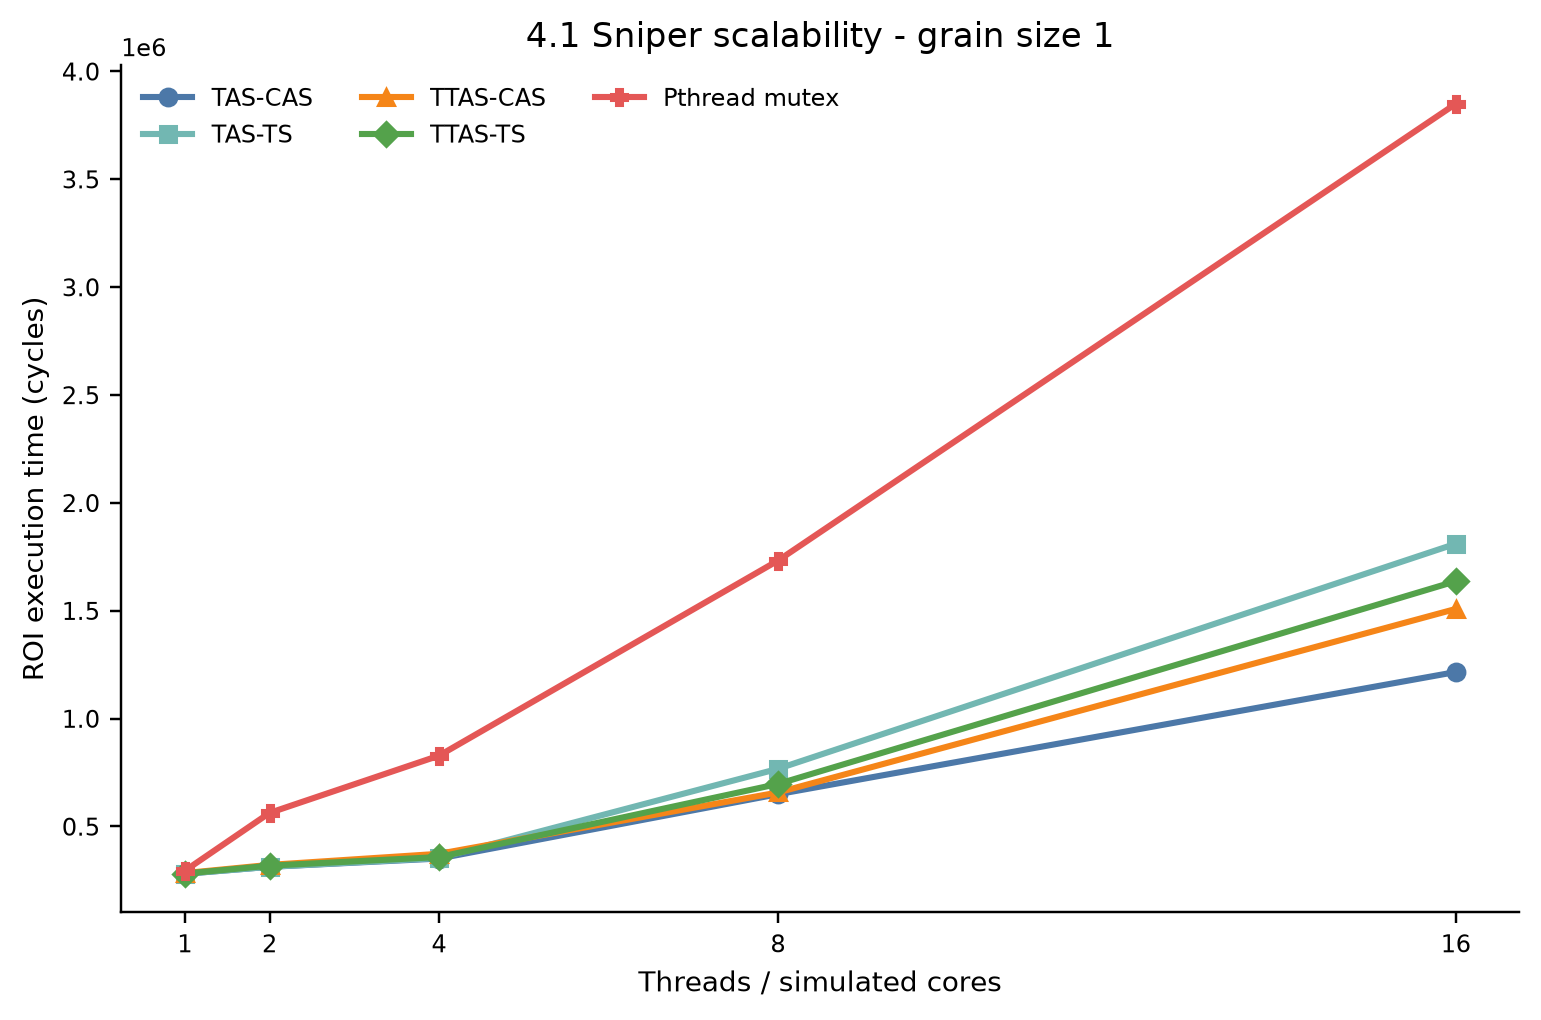
\includegraphics[width=0.82\textwidth]{4_1_sniper_cycles_grain_1.png}
\caption{Κύκλοι εκτέλεσης Sniper για \code{grain=1}.}
\label{fig:sniper-cycles-grain-1}
\end{figure}

Από το Διάγραμμα~\ref{fig:sniper-cycles-grain-1} προκύπτει ότι η υλοποίηση \code{MUTEX} έχει σημαντικά μεγαλύτερο κόστος καθώς αυξάνεται το πλήθος των νημάτων. Για 16 νήματα απαιτεί 3{,}848{,}985 κύκλους, ενώ η καλύτερη υλοποίηση spinlock, δηλαδή η \code{TAS_CAS}, απαιτεί 1{,}215{,}417 κύκλους. Αυτό δείχνει ότι, στη συγκεκριμένη μικρή κρίσιμη περιοχή και μέσα στο μοντέλο του Sniper, το mutex της Pthreads έχει μεγαλύτερο overhead από τα απλά spinlocks.

Για \code{grain=1}, η \code{TAS_CAS} είναι η καλύτερη επιλογή από τα 2 έως τα 16 νήματα ως προς τους κύκλους. Η \code{TAS_TS} είναι οριακά καλύτερη μόνο στη μονονηματική περίπτωση, όπου δεν υπάρχει πραγματικό contention. Οι εκδόσεις TTAS δεν υπερισχύουν εδώ, παρότι θεωρητικά μειώνουν τις ατομικές εγγραφές, επειδή το επιπλέον path spin-on-read αυξάνει σημαντικά τον αριθμό εντολών χωρίς να υπάρχει αρκετό υπολογιστικό έργο μέσα στην κρίσιμη περιοχή ώστε να αντισταθμιστεί αυτό το κόστος.

\subsection{Κύκλοι εκτέλεσης για \code{grain=10}}

Στην περίπτωση \code{grain=10}, η κρίσιμη περιοχή έχει μεγαλύτερη διάρκεια. Το lock κρατείται περισσότερο χρόνο, αλλά το κόστος της απόκτησης επιμερίζεται σε μεγαλύτερο υπολογιστικό έργο. Αυτό αλλάζει την ισορροπία μεταξύ των υλοποιήσεων TAS και TTAS.

\begin{figure}[htbp]
\centering
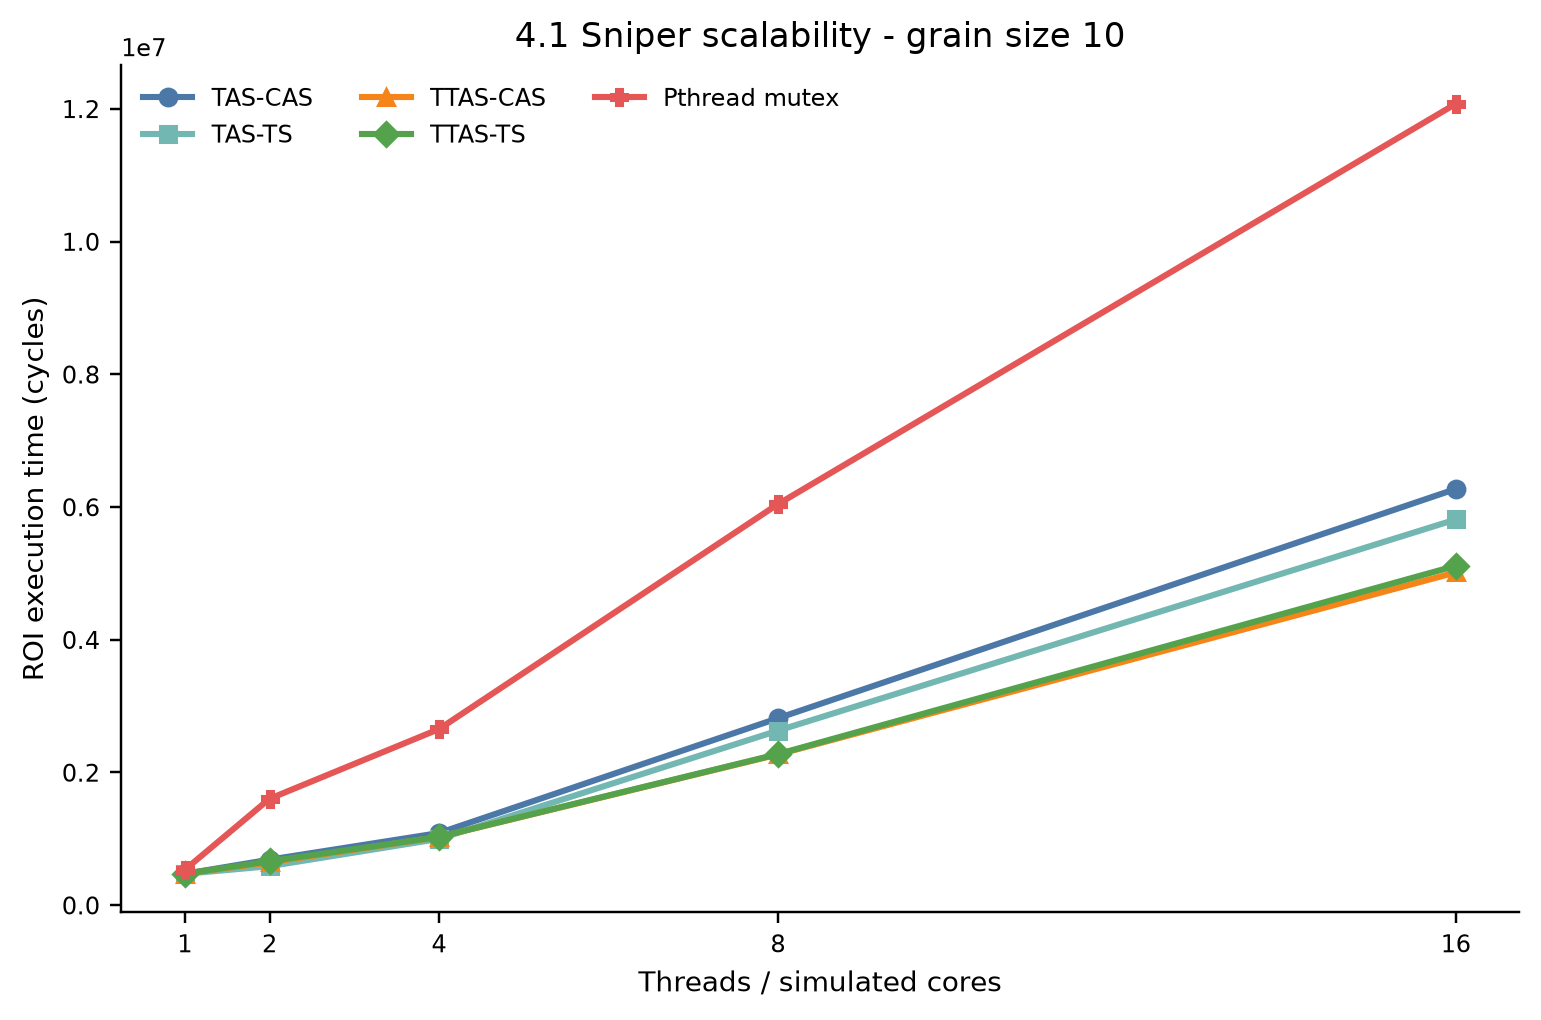
\includegraphics[width=0.82\textwidth]{4_1_sniper_cycles_grain_10.png}
\caption{Κύκλοι εκτέλεσης Sniper για \code{grain=10}.}
\label{fig:sniper-cycles-grain-10}
\end{figure}

Στο Διάγραμμα~\ref{fig:sniper-cycles-grain-10}, για μικρό αριθμό νημάτων η \code{TAS_TS} εμφανίζει την καλύτερη συμπεριφορά. Συγκεκριμένα, για 2 νήματα εκτελείται σε (586{,}831) κύκλους και για 4 νήματα σε (997{,}577) κύκλους. Για 8 και 16 νήματα, όμως, οι εκδόσεις TTAS γίνονται ταχύτερες ως προς τους κύκλους: η \code{TTAS_CAS} φτάνει τους 2{,}269{,}909 κύκλους στα 8 νήματα και τους 5{,}013{,}364 κύκλους στα 16 νήματα.

Η αλλαγή αυτή είναι αναμενόμενη. Όσο αυξάνεται το contention, τα locks TAS προκαλούν συνεχείς ατομικές προσβάσεις στη cache line του lock. Αντίθετα, το TTAS επιτρέπει στα νήματα που περιμένουν να κάνουν spin με απλές αναγνώσεις όσο το lock παραμένει κατειλημμένο. Έτσι, μειώνεται η πίεση στο coherence protocol ως προς τις μεταβάσεις write-intent. Ωστόσο, όπως θα φανεί στους ενεργειακούς πίνακες, αυτό δεν σημαίνει ότι το TTAS είναι πάντα ενεργειακά καλύτερο.

\subsection{Κύκλοι εκτέλεσης για \code{grain=100}}

Η περίπτωση \code{grain=100} έχει τη μεγαλύτερη κρίσιμη περιοχή. Εδώ το κόστος του lock παραμένει σημαντικό, αλλά το μεγαλύτερο μέρος του χρόνου αναλώνεται πλέον στην προστατευμένη υπολογιστική εργασία. Τα αποτελέσματα φαίνονται στο Διάγραμμα~\ref{fig:sniper-cycles-grain-100}.

\begin{figure}[htbp]
\centering
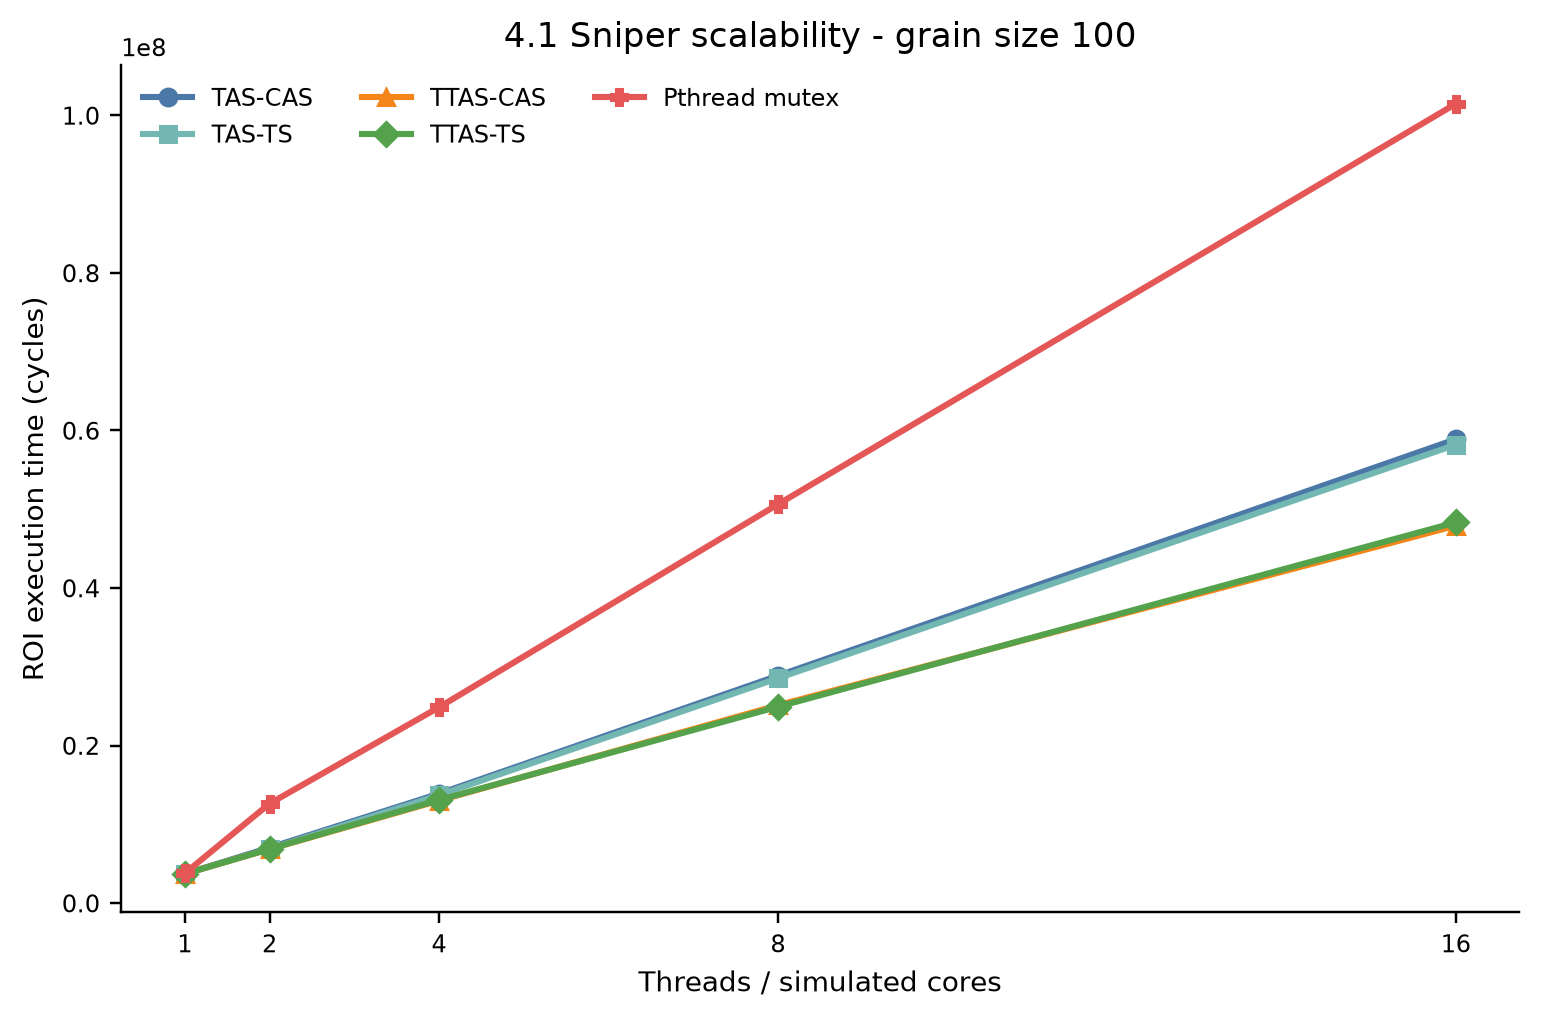
\includegraphics[width=0.82\textwidth]{4_1_sniper_cycles_grain_100.png}
\caption{Κύκλοι εκτέλεσης Sniper για \code{grain=100}.}
\label{fig:sniper-cycles-grain-100}
\end{figure}

Για \code{grain=100}, οι υλοποιήσεις TTAS εμφανίζουν πλέον σαφή πλεονεκτήματα στους κύκλους για περισσότερα νήματα. Για 4 νήματα, η \code{TTAS_CAS} έχει (13{,}008{,}408) κύκλους, ενώ η \code{TAS_CAS} έχει (13{,}883{,}464) και η \code{MUTEX} (24{,}854{,}676). Για 16 νήματα, η \code{TTAS_CAS} φτάνει τους (47{,}903{,}789) κύκλους, ενώ η \code{MUTEX} απαιτεί (101{,}465{,}177) κύκλους.

Το αποτέλεσμα αυτό δείχνει ότι, όταν η κρίσιμη περιοχή είναι αρκετά μεγάλη, η μείωση του coherence traffic κατά την αναμονή έχει ουσιαστική επίδραση στην απόδοση. Παρ' όλα αυτά, η βελτίωση στους κύκλους δεν είναι γραμμική ως προς τα νήματα. Το πρόγραμμα παραμένει ουσιαστικά σειριοποιημένο γύρω από μία κοινή κρίσιμη περιοχή, επομένως η αύξηση των νημάτων αυξάνει κυρίως τον ανταγωνισμό και όχι την πραγματική παράλληλη εργασία.

\subsection{Πλήρη αριθμητικά αποτελέσματα Sniper}

Οι Πίνακες~\ref{tab:sniper-full-grain-1}, \ref{tab:sniper-full-grain-10} και \ref{tab:sniper-full-grain-100} παραθέτουν τα πλήρη αριθμητικά αποτελέσματα των προσομοιώσεων Sniper της ενότητας 4.1. Περιλαμβάνονται οι συνολικές εντολές, οι συνολικοί κύκλοι, ο υπολογιζόμενος χρόνος εκτέλεσης, η ισχύς, η ενέργεια, τα $EDP$ και $ED^2P$.

\begin{table}[htbp]
\centering
\scriptsize
\caption{Πλήρη αριθμητικά αποτελέσματα Sniper για \code{grain=1}.}
\label{tab:sniper-full-grain-1}
\resizebox{\textwidth}{!}{
\begin{tabular}{P{2.3cm} P{1.4cm} P{2.1cm} P{2.1cm} P{1.8cm} P{1.7cm} P{1.7cm} P{1.8cm} P{2.0cm}}
\toprule
\textbf{Υλοποίηση} & \textbf{Νήματα} & \textbf{Instr.} & \textbf{Cycles} & \textbf{Runtime (ms)} & \textbf{Power (W)} & \textbf{Energy (J)} & \textbf{EDP (J s)} & \textbf{ED$^2$P (J s$^2$)} \\
\midrule
\code{MUTEX} & 1 & 86992 & 294087 & 0.110559 & 1227.62 & 0.14 & 1.54783e-05 & 1.711000e-09 \\
\code{TAS_CAS} & 1 & 71186 & 280347 & 0.105394 & 1009.21 & 0.11 & 1.15933e-05 & 1.222000e-09 \\
\code{TAS_TS} & 1 & 70186 & 280050 & 0.105282 & 987.25 & 0.10 & 1.05282e-05 & 1.108000e-09 \\
\code{TTAS_CAS} & 1 & 75186 & 283543 & 0.106595 & 1044.42 & 0.11 & 1.17254e-05 & 1.250000e-09 \\
\code{TTAS_TS} & 1 & 74186 & 281145 & 0.105694 & 1030.02 & 0.11 & 1.16263e-05 & 1.229000e-09 \\
\midrule
\code{MUTEX} & 2 & 175624 & 562394 & 0.211427 & 1333.25 & 0.28 & 5.91996e-05 & 1.251600e-08 \\
\code{TAS_CAS} & 2 & 177845 & 312642 & 0.117535 & 2309.37 & 0.27 & 3.17345e-05 & 3.730000e-09 \\
\code{TAS_TS} & 2 & 231579 & 312738 & 0.117571 & 2908.69 & 0.34 & 3.99741e-05 & 4.700000e-09 \\
\code{TTAS_CAS} & 2 & 215474 & 321551 & 0.120884 & 2499.35 & 0.30 & 3.62652e-05 & 4.384000e-09 \\
\code{TTAS_TS} & 2 & 237421 & 317926 & 0.119521 & 2731.99 & 0.33 & 3.94419e-05 & 4.714000e-09 \\
\midrule
\code{MUTEX} & 4 & 353002 & 827685 & 0.311160 & 1868.37 & 0.58 & 0.000180473 & 5.615600e-08 \\
\code{TAS_CAS} & 4 & 404798 & 350986 & 0.131950 & 4737.86 & 0.63 & 8.31285e-05 & 1.096900e-08 \\
\code{TAS_TS} & 4 & 810685 & 353366 & 0.132845 & 8998.82 & 1.20 & 0.000159414 & 2.117700e-08 \\
\code{TTAS_CAS} & 4 & 792057 & 372840 & 0.140166 & 7483.64 & 1.05 & 0.000147174 & 2.062900e-08 \\
\code{TTAS_TS} & 4 & 749502 & 357914 & 0.134554 & 7364.69 & 0.99 & 0.000133208 & 1.792400e-08 \\
\midrule
\code{MUTEX} & 8 & 697287 & 1731712 & 0.651020 & 1931.64 & 1.26 & 0.000820285 & 5.340220e-07 \\
\code{TAS_CAS} & 8 & 901262 & 649149 & 0.244041 & 5880.91 & 1.44 & 0.000351419 & 8.576100e-08 \\
\code{TAS_TS} & 8 & 1427115 & 766709 & 0.288237 & 7476.85 & 2.16 & 0.000622592 & 1.794540e-07 \\
\code{TTAS_CAS} & 8 & 4047240 & 657062 & 0.247016 & 20858.52 & 5.15 & 0.00127213 & 3.142370e-07 \\
\code{TTAS_TS} & 8 & 4331524 & 696532 & 0.261854 & 20989.01 & 5.50 & 0.0014402 & 3.771210e-07 \\
\midrule
\code{MUTEX} & 16 & 1409918 & 3848985 & 1.446987 & 2130.50 & 3.08 & 0.00445672 & 6.448816e-06 \\
\code{TAS_CAS} & 16 & 1908234 & 1215417 & 0.456924 & 6988.34 & 3.19 & 0.00145759 & 6.660070e-07 \\
\code{TAS_TS} & 16 & 2612617 & 1809916 & 0.680420 & 6215.03 & 4.23 & 0.00287818 & 1.958369e-06 \\
\code{TTAS_CAS} & 16 & 8304496 & 1507798 & 0.566842 & 19022.18 & 10.78 & 0.00611056 & 3.463720e-06 \\
\code{TTAS_TS} & 16 & 10683832 & 1636322 & 0.615159 & 22294.07 & 13.71 & 0.00843383 & 5.188146e-06 \\
\bottomrule
\end{tabular}
}
\end{table}

\begin{table}[htbp]
\centering
\scriptsize
\caption{Πλήρη αριθμητικά αποτελέσματα Sniper για \code{grain=10}.}
\label{tab:sniper-full-grain-10}
\resizebox{\textwidth}{!}{
\begin{tabular}{P{2.3cm} P{1.4cm} P{2.1cm} P{2.1cm} P{1.8cm} P{1.7cm} P{1.7cm} P{1.8cm} P{2.0cm}}
\toprule
\textbf{Υλοποίηση} & \textbf{Νήματα} & \textbf{Instr.} & \textbf{Cycles} & \textbf{Runtime (ms)} & \textbf{Power (W)} & \textbf{Energy (J)} & \textbf{EDP (J s)} & \textbf{ED$^2$P (J s$^2$)} \\
\midrule
\code{MUTEX} & 1 & 203992 & 532157 & 0.200059 & 1527.26 & 0.31 & 6.20183e-05 & 1.240700e-08 \\
\code{TAS_CAS} & 1 & 188186 & 471885 & 0.177401 & 1551.99 & 0.28 & 4.96723e-05 & 8.812000e-09 \\
\code{TAS_TS} & 1 & 187186 & 471330 & 0.177192 & 1540.11 & 0.27 & 4.78418e-05 & 8.477000e-09 \\
\code{TTAS_CAS} & 1 & 192186 & 474017 & 0.178202 & 1572.76 & 0.28 & 4.98966e-05 & 8.892000e-09 \\
\code{TTAS_TS} & 1 & 191186 & 472949 & 0.177801 & 1562.61 & 0.28 & 4.97843e-05 & 8.852000e-09 \\
\midrule
\code{MUTEX} & 2 & 420846 & 1602535 & 0.602457 & 1100.37 & 0.66 & 0.000397622 & 2.395500e-07 \\
\code{TAS_CAS} & 2 & 734687 & 685042 & 0.257535 & 4422.40 & 1.14 & 0.00029359 & 7.561000e-08 \\
\code{TAS_TS} & 2 & 763970 & 586831 & 0.220613 & 5072.82 & 1.12 & 0.000247087 & 5.451100e-08 \\
\code{TTAS_CAS} & 2 & 942184 & 645644 & 0.242724 & 5141.84 & 1.25 & 0.000303405 & 7.364400e-08 \\
\code{TTAS_TS} & 2 & 993914 & 660802 & 0.248422 & 5271.67 & 1.31 & 0.000325433 & 8.084500e-08 \\
\midrule
\code{MUTEX} & 4 & 843994 & 2652682 & 0.997249 & 1393.06 & 1.39 & 0.00138618 & 1.382363e-06 \\
\code{TAS_CAS} & 4 & 2172083 & 1086014 & 0.408276 & 8433.96 & 3.44 & 0.00140447 & 5.734110e-07 \\
\code{TAS_TS} & 4 & 4850087 & 997577 & 0.375029 & 19018.22 & 7.13 & 0.00267396 & 1.002811e-06 \\
\code{TTAS_CAS} & 4 & 4329630 & 1026483 & 0.385896 & 14296.51 & 5.52 & 0.00213015 & 8.220150e-07 \\
\code{TTAS_TS} & 4 & 4692133 & 1027668 & 0.386342 & 15418.71 & 5.96 & 0.0023026 & 8.895900e-07 \\
\midrule
\code{MUTEX} & 8 & 1699855 & 6041941 & 2.271407 & 1407.57 & 3.20 & 0.0072685 & 1.650973e-05 \\
\code{TAS_CAS} & 8 & 4483319 & 2816003 & 1.058648 & 6914.05 & 7.32 & 0.0077493 & 8.203785e-06 \\
\code{TAS_TS} & 8 & 4370003 & 2629017 & 0.988352 & 6723.87 & 6.65 & 0.00657254 & 6.495984e-06 \\
\code{TTAS_CAS} & 8 & 23777850 & 2269909 & 0.853349 & 34837.31 & 29.73 & 0.0253701 & 2.164952e-05 \\
\code{TTAS_TS} & 8 & 24802976 & 2275260 & 0.855361 & 36214.71 & 30.98 & 0.0264991 & 2.266628e-05 \\
\midrule
\code{MUTEX} & 16 & 3436401 & 12074521 & 4.539294 & 1764.97 & 8.01 & 0.0363597 & 1.650476e-04 \\
\code{TAS_CAS} & 16 & 9663888 & 6271043 & 2.357535 & 7073.72 & 16.68 & 0.0393237 & 9.270696e-05 \\
\code{TAS_TS} & 16 & 8924545 & 5811106 & 2.184627 & 6589.52 & 14.40 & 0.0314586 & 6.872537e-05 \\
\code{TTAS_CAS} & 16 & 75468786 & 5013364 & 1.884724 & 50091.83 & 94.41 & 0.177937 & 3.353617e-04 \\
\code{TTAS_TS} & 16 & 80638431 & 5112844 & 1.922122 & 52419.33 & 100.76 & 0.193673 & 3.722632e-04 \\
\bottomrule
\end{tabular}
}
\end{table}

\begin{table}[htbp]
\centering
\scriptsize
\caption{Πλήρη αριθμητικά αποτελέσματα Sniper για \code{grain=100}.}
\label{tab:sniper-full-grain-100}
\resizebox{\textwidth}{!}{
\begin{tabular}{P{2.3cm} P{1.4cm} P{2.1cm} P{2.1cm} P{1.8cm} P{1.7cm} P{1.7cm} P{1.8cm} P{2.0cm}}
\toprule
\textbf{Υλοποίηση} & \textbf{Νήματα} & \textbf{Instr.} & \textbf{Cycles} & \textbf{Runtime (ms)} & \textbf{Power (W)} & \textbf{Energy (J)} & \textbf{EDP (J s)} & \textbf{ED$^2$P (J s$^2$)} \\
\midrule
\code{MUTEX} & 1 & 1373992 & 3772055 & 1.418066 & 1424.13 & 2.02 & 0.00286449 & 4.062041e-06 \\
\code{TAS_CAS} & 1 & 1358186 & 3711517 & 1.395307 & 1425.70 & 1.99 & 0.00277666 & 3.874294e-06 \\
\code{TAS_TS} & 1 & 1357186 & 3711228 & 1.395199 & 1424.07 & 1.99 & 0.00277645 & 3.873695e-06 \\
\code{TTAS_CAS} & 1 & 1362186 & 3714447 & 1.396409 & 1428.13 & 1.99 & 0.00277885 & 3.880417e-06 \\
\code{TTAS_TS} & 1 & 1361186 & 3712581 & 1.395707 & 1427.09 & 1.99 & 0.00277746 & 3.876516e-06 \\
\midrule
\code{MUTEX} & 2 & 2803694 & 12621207 & 4.744815 & 925.87 & 4.39 & 0.0208297 & 9.883325e-05 \\
\code{TAS_CAS} & 2 & 9275489 & 7031306 & 2.643348 & 5571.66 & 14.73 & 0.0389365 & 1.029228e-04 \\
\code{TAS_TS} & 2 & 17012075 & 6873880 & 2.584166 & 9680.81 & 25.02 & 0.0646558 & 1.670814e-04 \\
\code{TTAS_CAS} & 2 & 15087046 & 6845906 & 2.573649 & 7476.34 & 19.24 & 0.049517 & 1.274394e-04 \\
\code{TTAS_TS} & 2 & 15193757 & 6864119 & 2.580496 & 7506.52 & 19.37 & 0.0499842 & 1.289840e-04 \\
\midrule
\code{MUTEX} & 4 & 5621821 & 24854676 & 9.343863 & 1019.05 & 9.52 & 0.0889536 & 8.311700e-04 \\
\code{TAS_CAS} & 4 & 28576148 & 13883464 & 5.219348 & 8841.81 & 46.15 & 0.240873 & 1.257200e-03 \\
\code{TAS_TS} & 4 & 101902440 & 13694640 & 5.148361 & 29125.23 & 149.95 & 0.771997 & 3.974518e-03 \\
\code{TTAS_CAS} & 4 & 76970788 & 13008408 & 4.890379 & 19681.63 & 96.25 & 0.470699 & 2.301896e-03 \\
\code{TTAS_TS} & 4 & 76535264 & 13087651 & 4.920170 & 19453.83 & 95.72 & 0.470959 & 2.317197e-03 \\
\midrule
\code{MUTEX} & 8 & 11241978 & 50621466 & 19.030627 & 1160.06 & 22.08 & 0.420196 & 7.996598e-03 \\
\code{TAS_CAS} & 8 & 45828506 & 28857988 & 10.848868 & 6974.57 & 75.67 & 0.820934 & 8.906203e-03 \\
\code{TAS_TS} & 8 & 49350969 & 28540627 & 10.729559 & 7010.90 & 75.22 & 0.807077 & 8.659585e-03 \\
\code{TTAS_CAS} & 8 & 339083209 & 25112180 & 9.440669 & 44599.97 & 421.05 & 3.97499 & 3.752660e-02 \\
\code{TTAS_TS} & 8 & 336428559 & 24923547 & 9.369755 & 44586.47 & 417.76 & 3.91431 & 3.667611e-02 \\
\midrule
\code{MUTEX} & 16 & 22487445 & 101465177 & 38.144804 & 1502.72 & 57.32 & 2.18646 & 8.340209e-02 \\
\code{TAS_CAS} & 16 & 88371924 & 58883201 & 22.136542 & 6952.01 & 153.89 & 3.40659 & 7.541018e-02 \\
\code{TAS_TS} & 16 & 88846363 & 58190248 & 21.876033 & 6573.83 & 143.81 & 3.14599 & 6.882183e-02 \\
\code{TTAS_CAS} & 16 & 1319043480 & 47903789 & 18.008943 & 90747.01 & 1630.00 & 29.3546 & 5.286449e-01 \\
\code{TTAS_TS} & 16 & 1318346120 & 48329806 & 18.169100 & 89904.71 & 1630.00 & 29.6156 & 5.380894e-01 \\
\bottomrule
\end{tabular}
}
\end{table}

\FloatBarrier

\subsection{Ενεργειακή συμπεριφορά}

Η ανάλυση μόνο των κύκλων εκτέλεσης δεν αρκεί για να εξαχθεί ασφαλές συμπέρασμα. Οι υλοποιήσεις TTAS μπορούν να μειώνουν τον χρόνο εκτέλεσης σε αρκετές περιπτώσεις υψηλού contention, αλλά παράλληλα εκτελούν πολύ μεγάλο πλήθος εντολών λόγω του βρόχου spin-on-read. Αυτό φαίνεται καθαρά στους πίνακες: για παράδειγμα, στο \code{grain=100} και στα 16 νήματα, η \code{TTAS_CAS} εκτελεί 1{,}319{,}043{,}480 εντολές, ενώ η \code{TAS_TS} εκτελεί (88{,}846{,}363). Παρότι η \code{TTAS_CAS} έχει λιγότερους κύκλους, η εκτιμώμενη ενέργειά της φτάνει τα \(1630.00\,\mathrm{J}\), δηλαδή είναι πολύ μεγαλύτερη από τις αντίστοιχες TAS και MUTEX τιμές.

\begin{figure}[htbp]
\centering
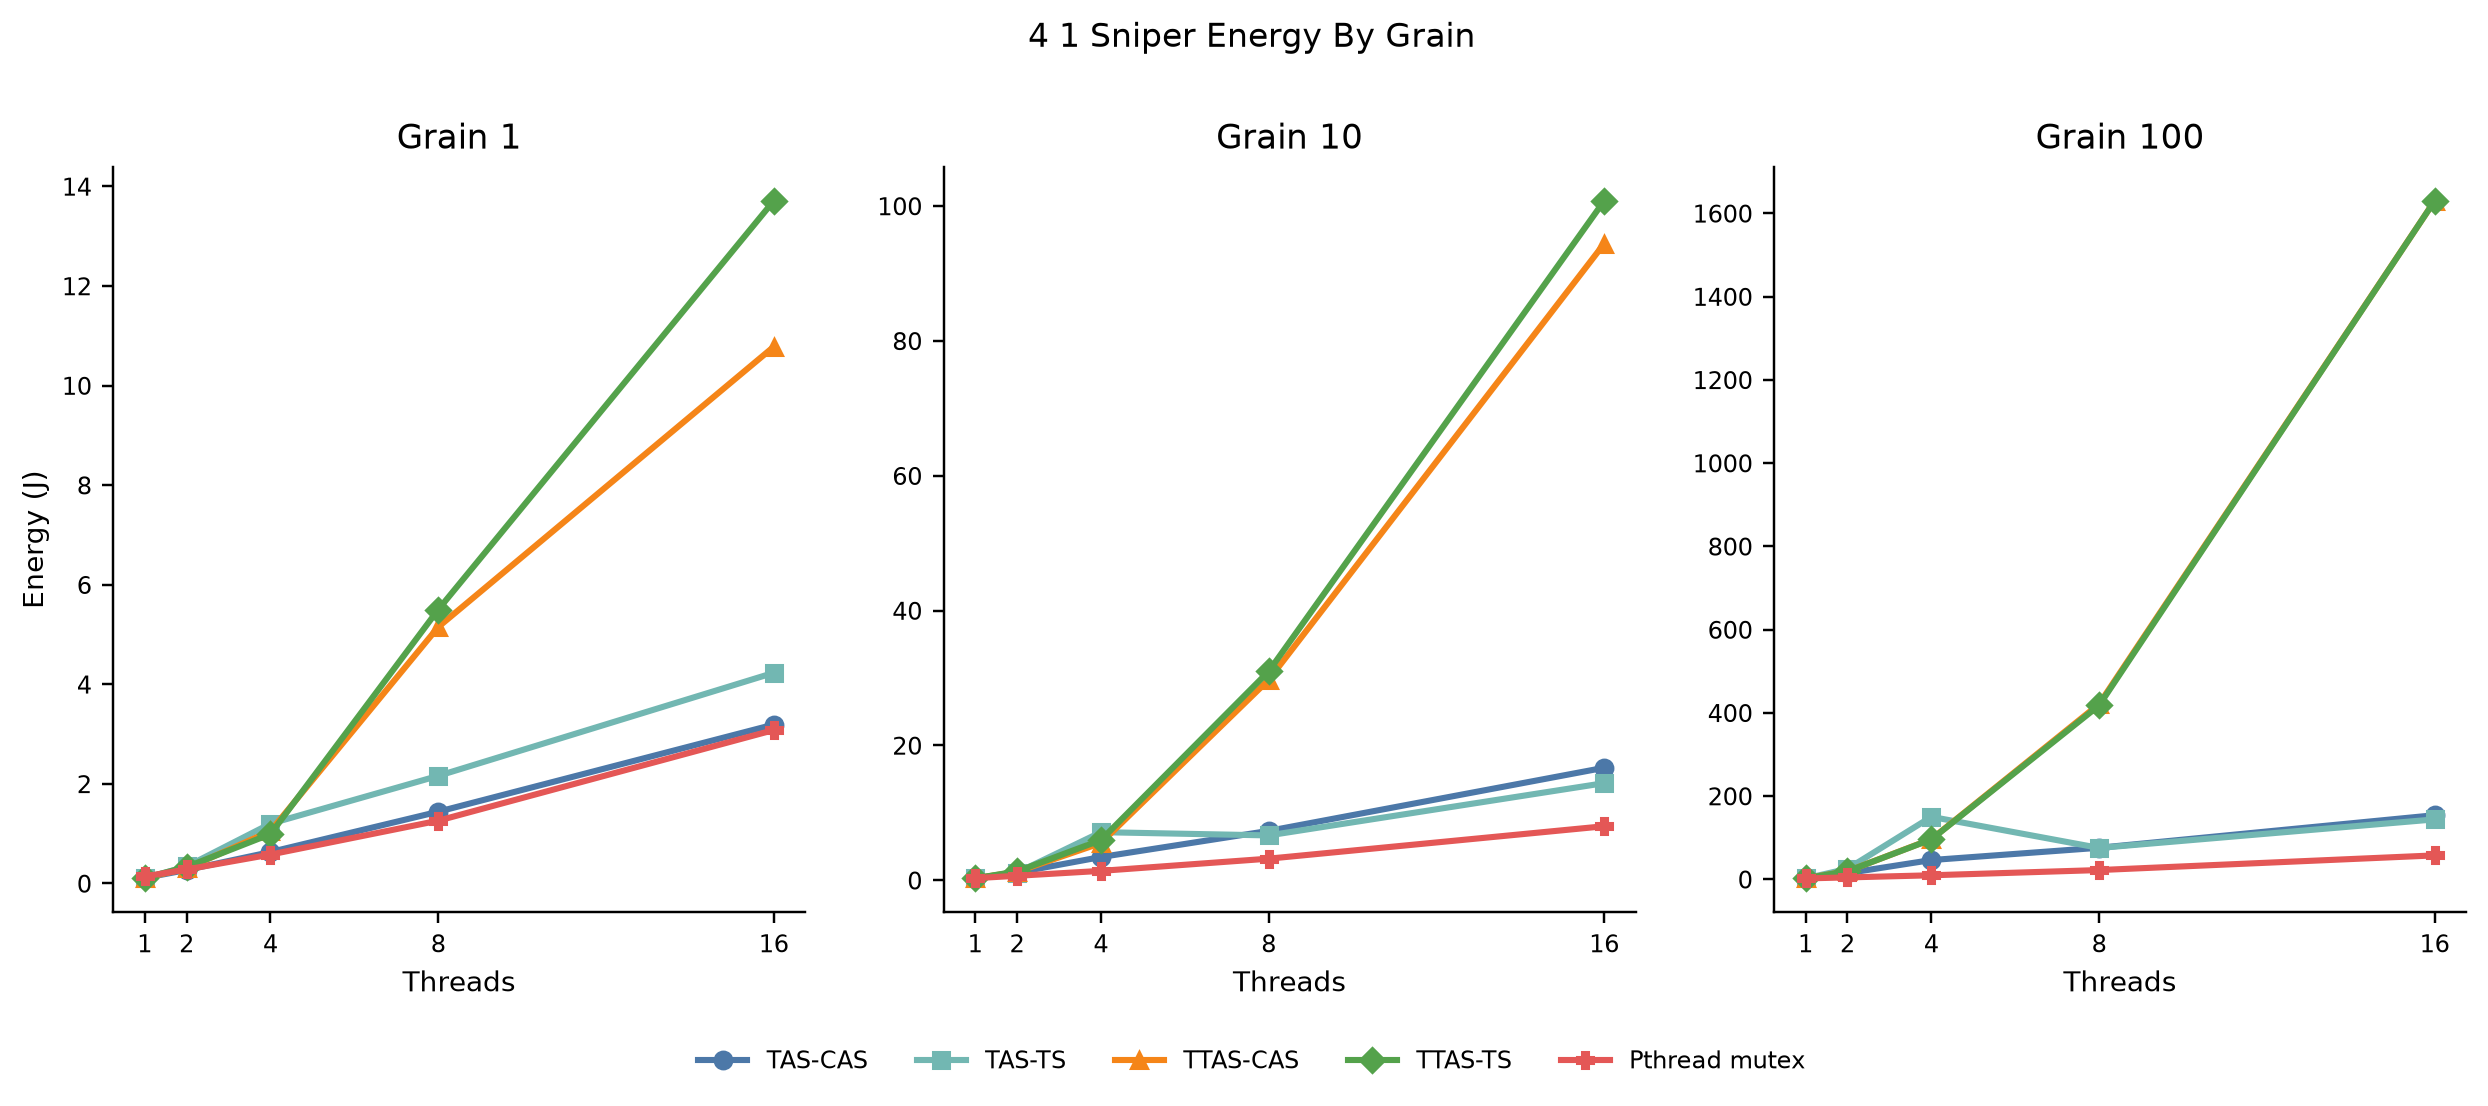
\includegraphics[width=0.84\textwidth]{4_1_sniper_energy_by_grain.png}
\caption{Ενέργεια Sniper/McPAT ανά τιμή grain.}
\label{fig:sniper-energy-by-grain}
\end{figure}

Το Διάγραμμα~\ref{fig:sniper-energy-by-grain} δείχνει ότι οι υλοποιήσεις TTAS έχουν έντονη ενεργειακή επιβάρυνση για μεγάλο αριθμό νημάτων και μεγάλο grain. Αυτό δεν αναιρεί την απόδοσή τους σε κύκλους, αλλά δείχνει ότι η αξιολόγηση ενός lock δεν πρέπει να βασίζεται σε μία μόνο μετρική. Ένας μηχανισμός που μειώνει τις ακριβές ατομικές εγγραφές μπορεί ταυτόχρονα να αυξήσει την πρόσθετη εκτέλεση εντολών και τη συνολική κατανάλωση.

\begin{figure}[htbp]
\centering
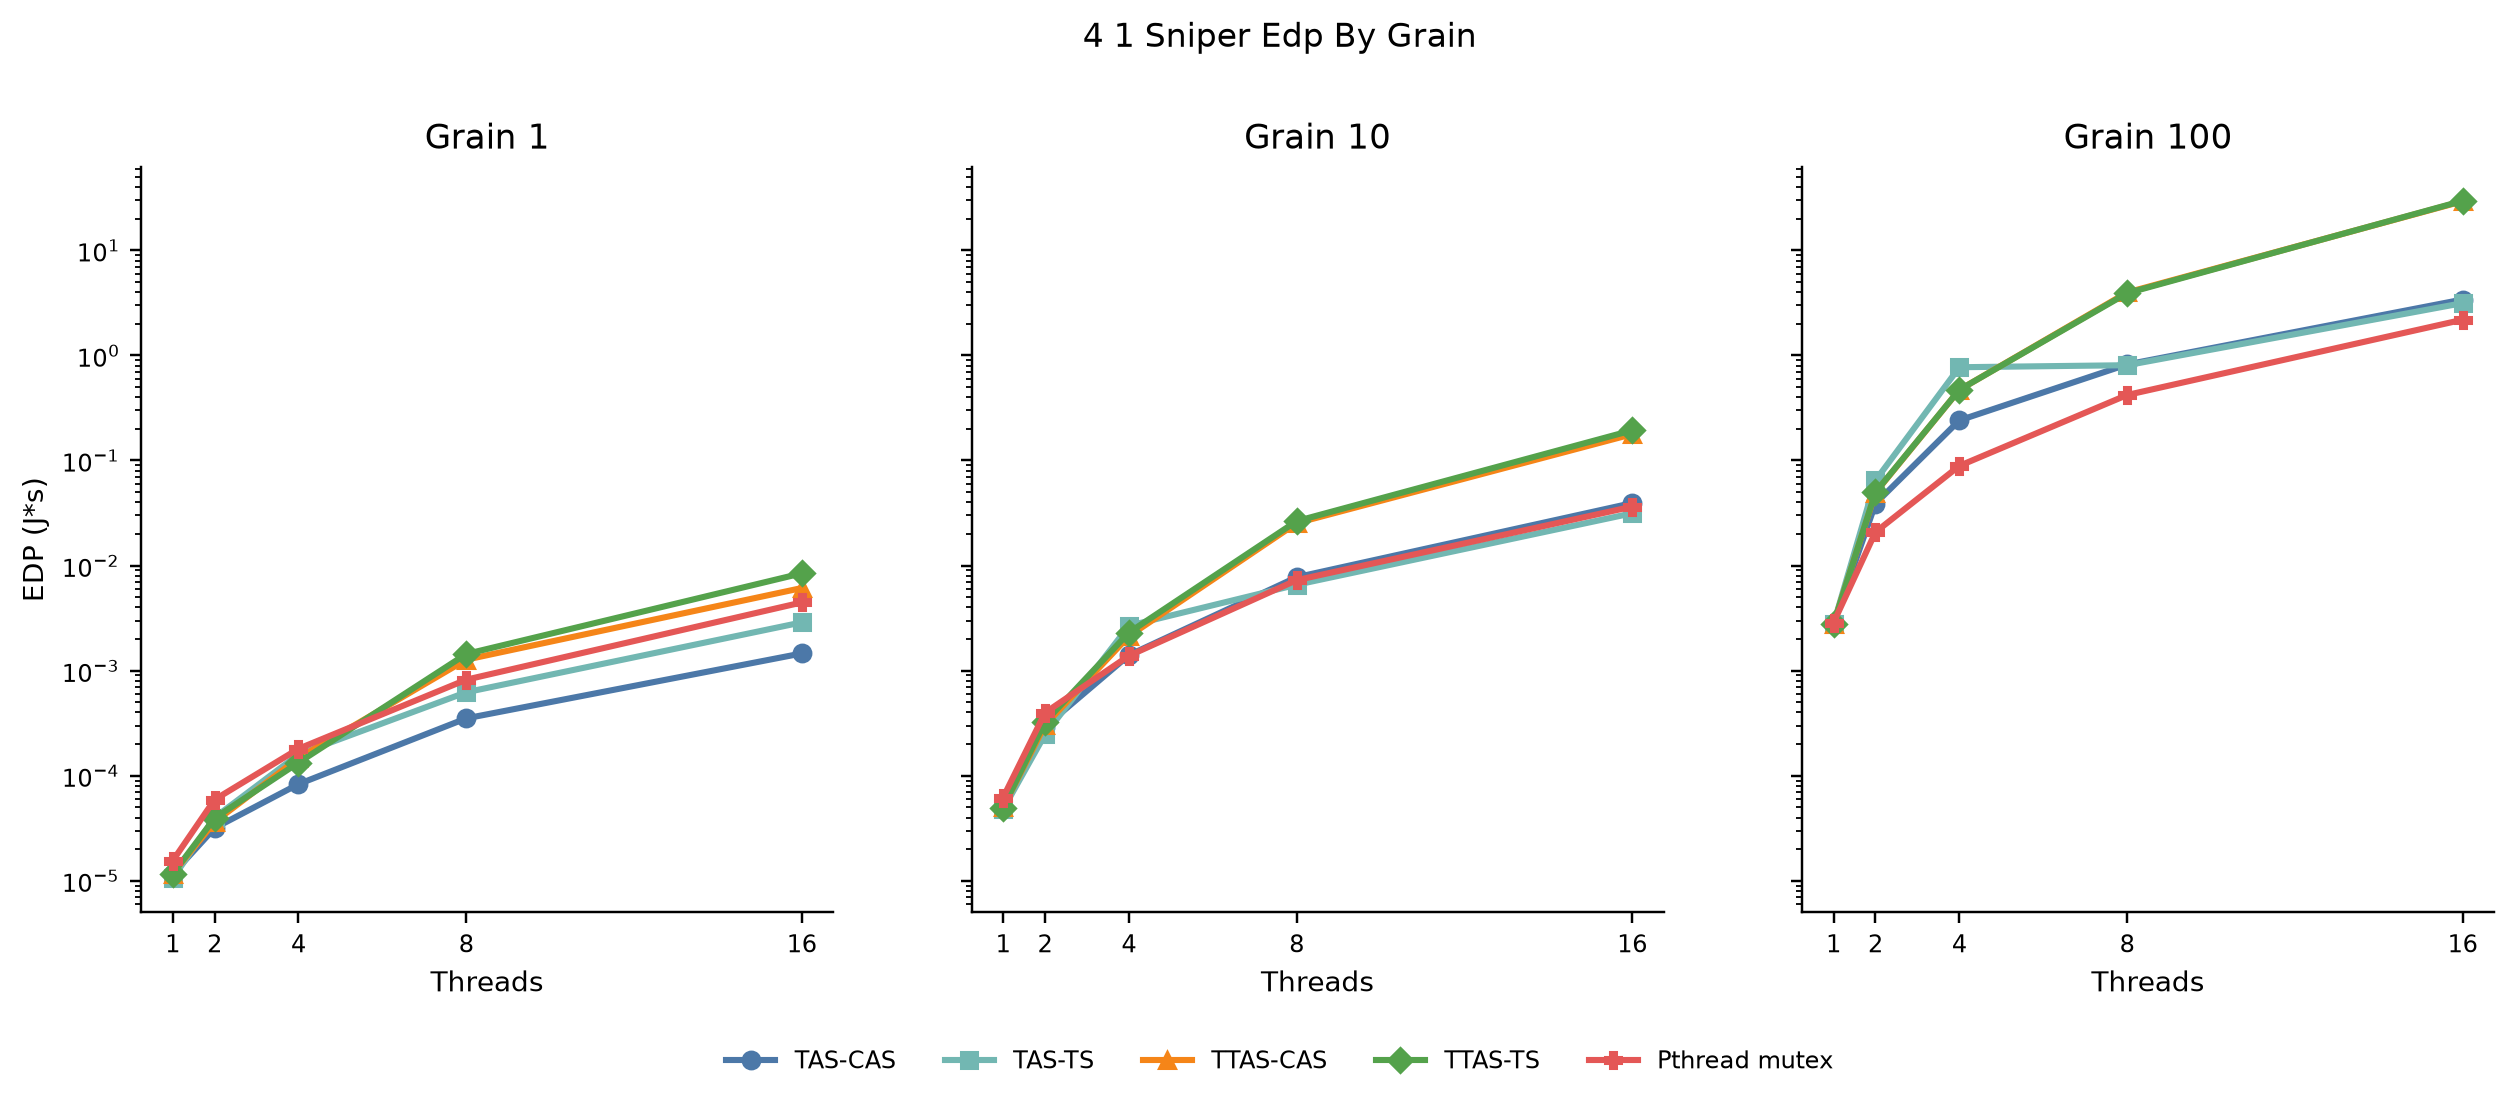
\includegraphics[width=0.84\textwidth]{4_1_sniper_edp_by_grain.png}
\caption{$EDP$ Sniper/McPAT ανά τιμή grain.}
\label{fig:sniper-edp-by-grain}
\end{figure}

Το $EDP$, που φαίνεται στο Διάγραμμα~\ref{fig:sniper-edp-by-grain}, συνδυάζει τον χρόνο και την ενέργεια. Για μικρή τιμή grain, η \code{TAS_CAS} είναι συνήθως η καλύτερη επιλογή, επειδή συνδυάζει μικρό χρόνο εκτέλεσης και σχετικά περιορισμένη ενέργεια. Για μεγαλύτερη τιμή grain, οι υλοποιήσεις TTAS βελτιώνουν τους κύκλους, αλλά το ενεργειακό κόστος τους αυξάνεται τόσο πολύ ώστε το $EDP$ τους γίνεται χειρότερο.

\begin{figure}[htbp]
\centering
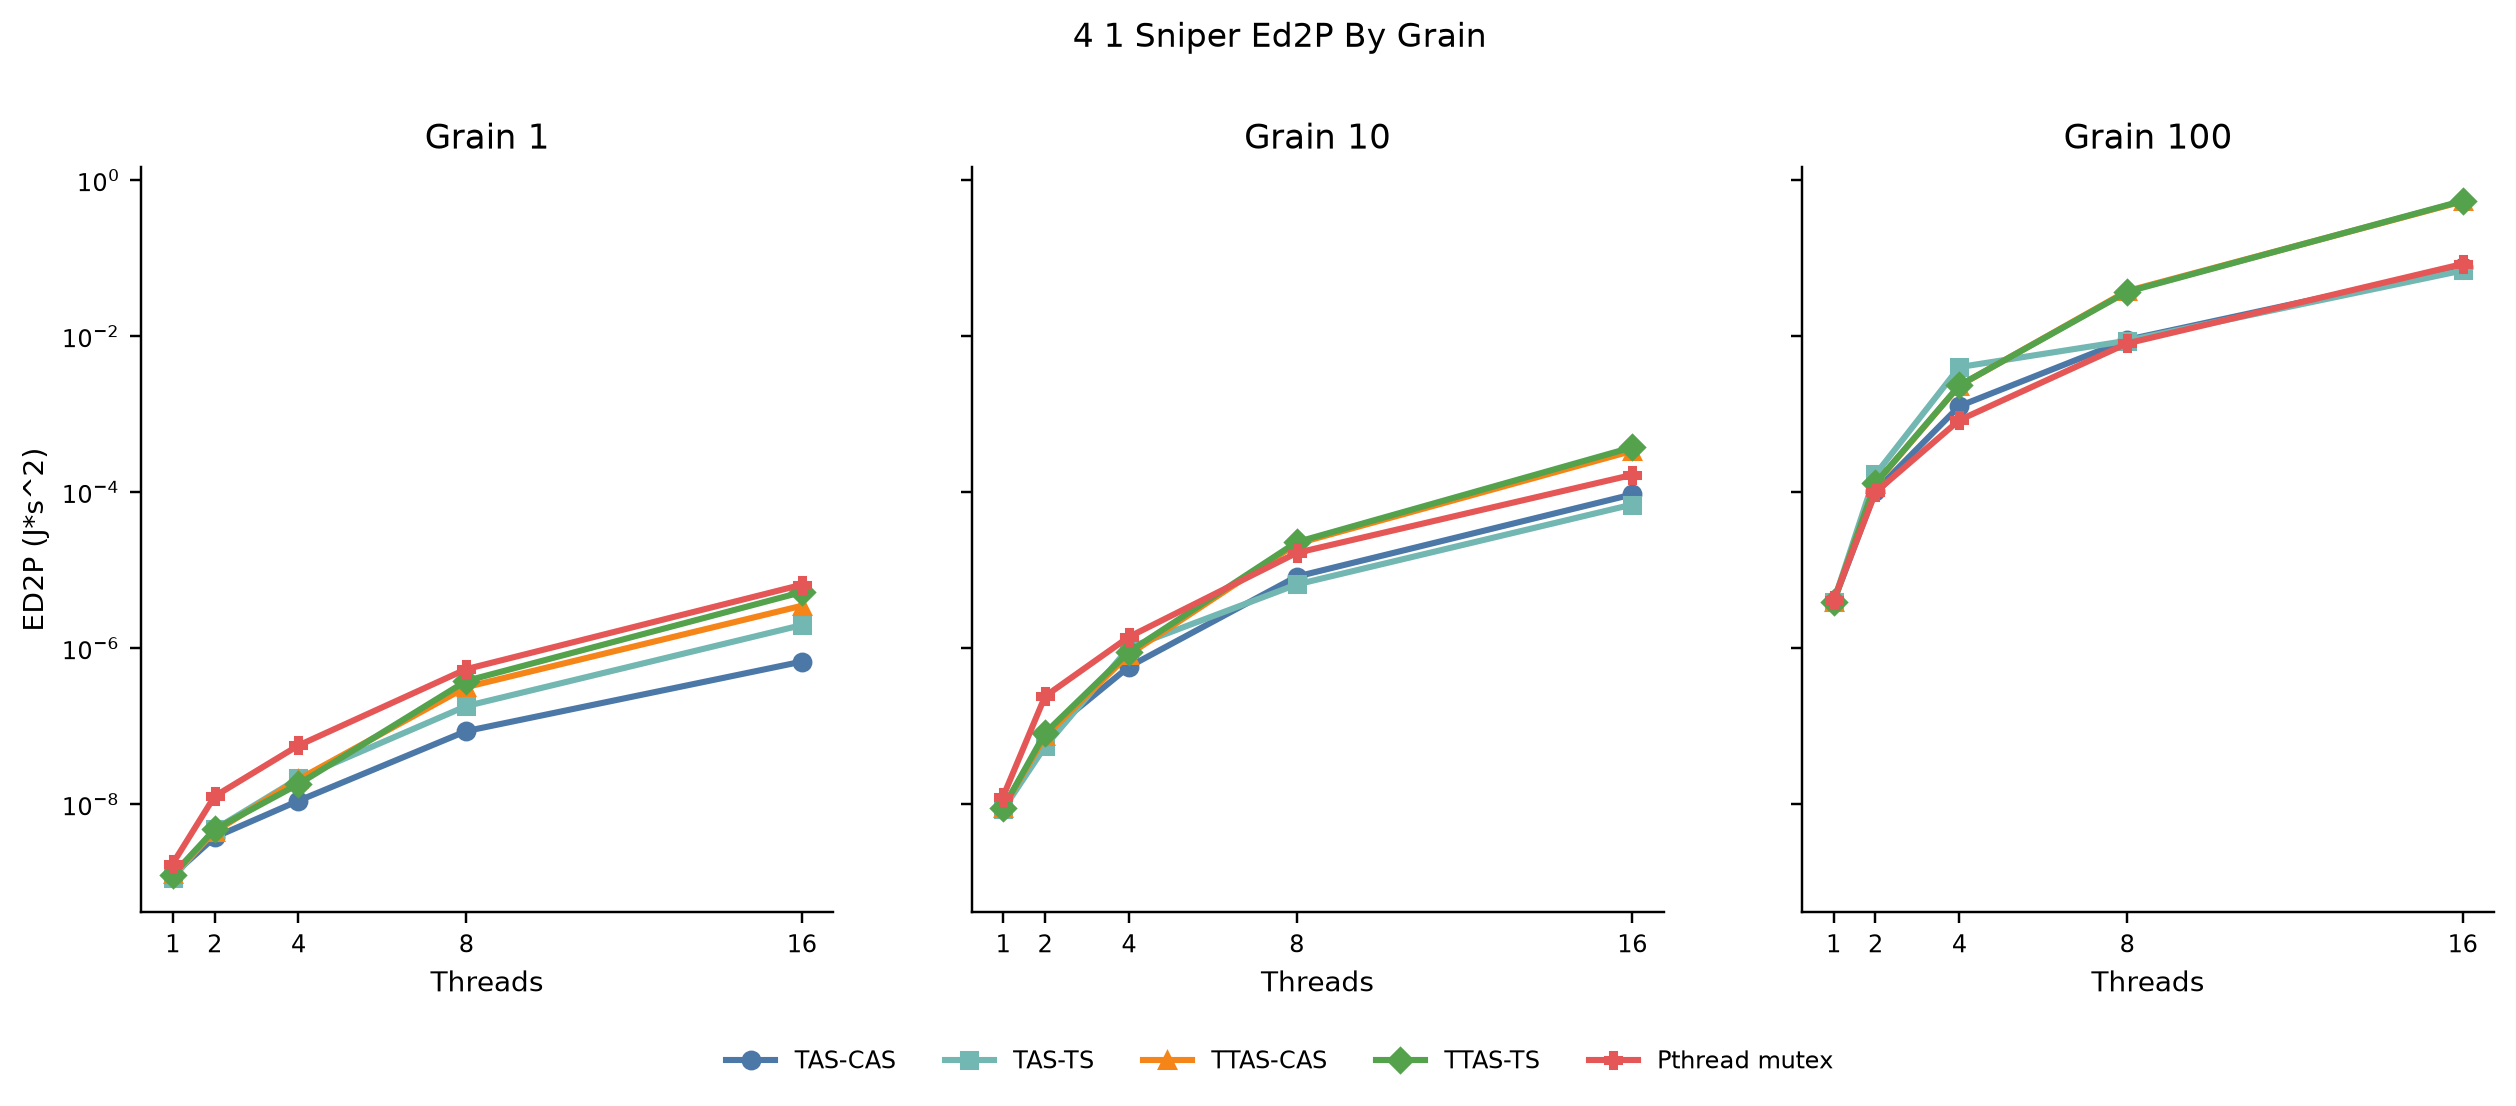
\includegraphics[width=0.84\textwidth]{4_1_sniper_ed2p_by_grain.png}
\caption{$ED^2P$ Sniper/McPAT ανά τιμή grain.}
\label{fig:sniper-ed2p-by-grain}
\end{figure}

Το $ED^2P$, στο Διάγραμμα~\ref{fig:sniper-ed2p-by-grain}, δίνει μεγαλύτερο βάρος στον χρόνο εκτέλεσης. Ακόμη και έτσι, οι υλοποιήσεις TTAS δεν είναι πάντα προτιμότερες, επειδή η ενεργειακή τους αύξηση είναι πολύ μεγάλη στις περιπτώσεις με πολλά νήματα. Αυτό είναι ιδιαίτερα εμφανές στα 16 νήματα και \code{grain=100}, όπου οι \code{TTAS_CAS} και \code{TTAS_TS} έχουν μεν τους μικρότερους κύκλους, αλλά τα μεγαλύτερα $EDP$ και $ED^2P$.

\subsection{Σχέση χρόνου και ενέργειας}

Για πιο συνολική ερμηνεία, χρησιμοποιήθηκε και το διάγραμμα χρόνου--ενέργειας. Σε ένα τέτοιο διάγραμμα, το ιδανικό σημείο βρίσκεται χαμηλά και αριστερά: χαμηλός χρόνος εκτέλεσης και χαμηλή ενέργεια.

\begin{figure}[htbp]
\centering
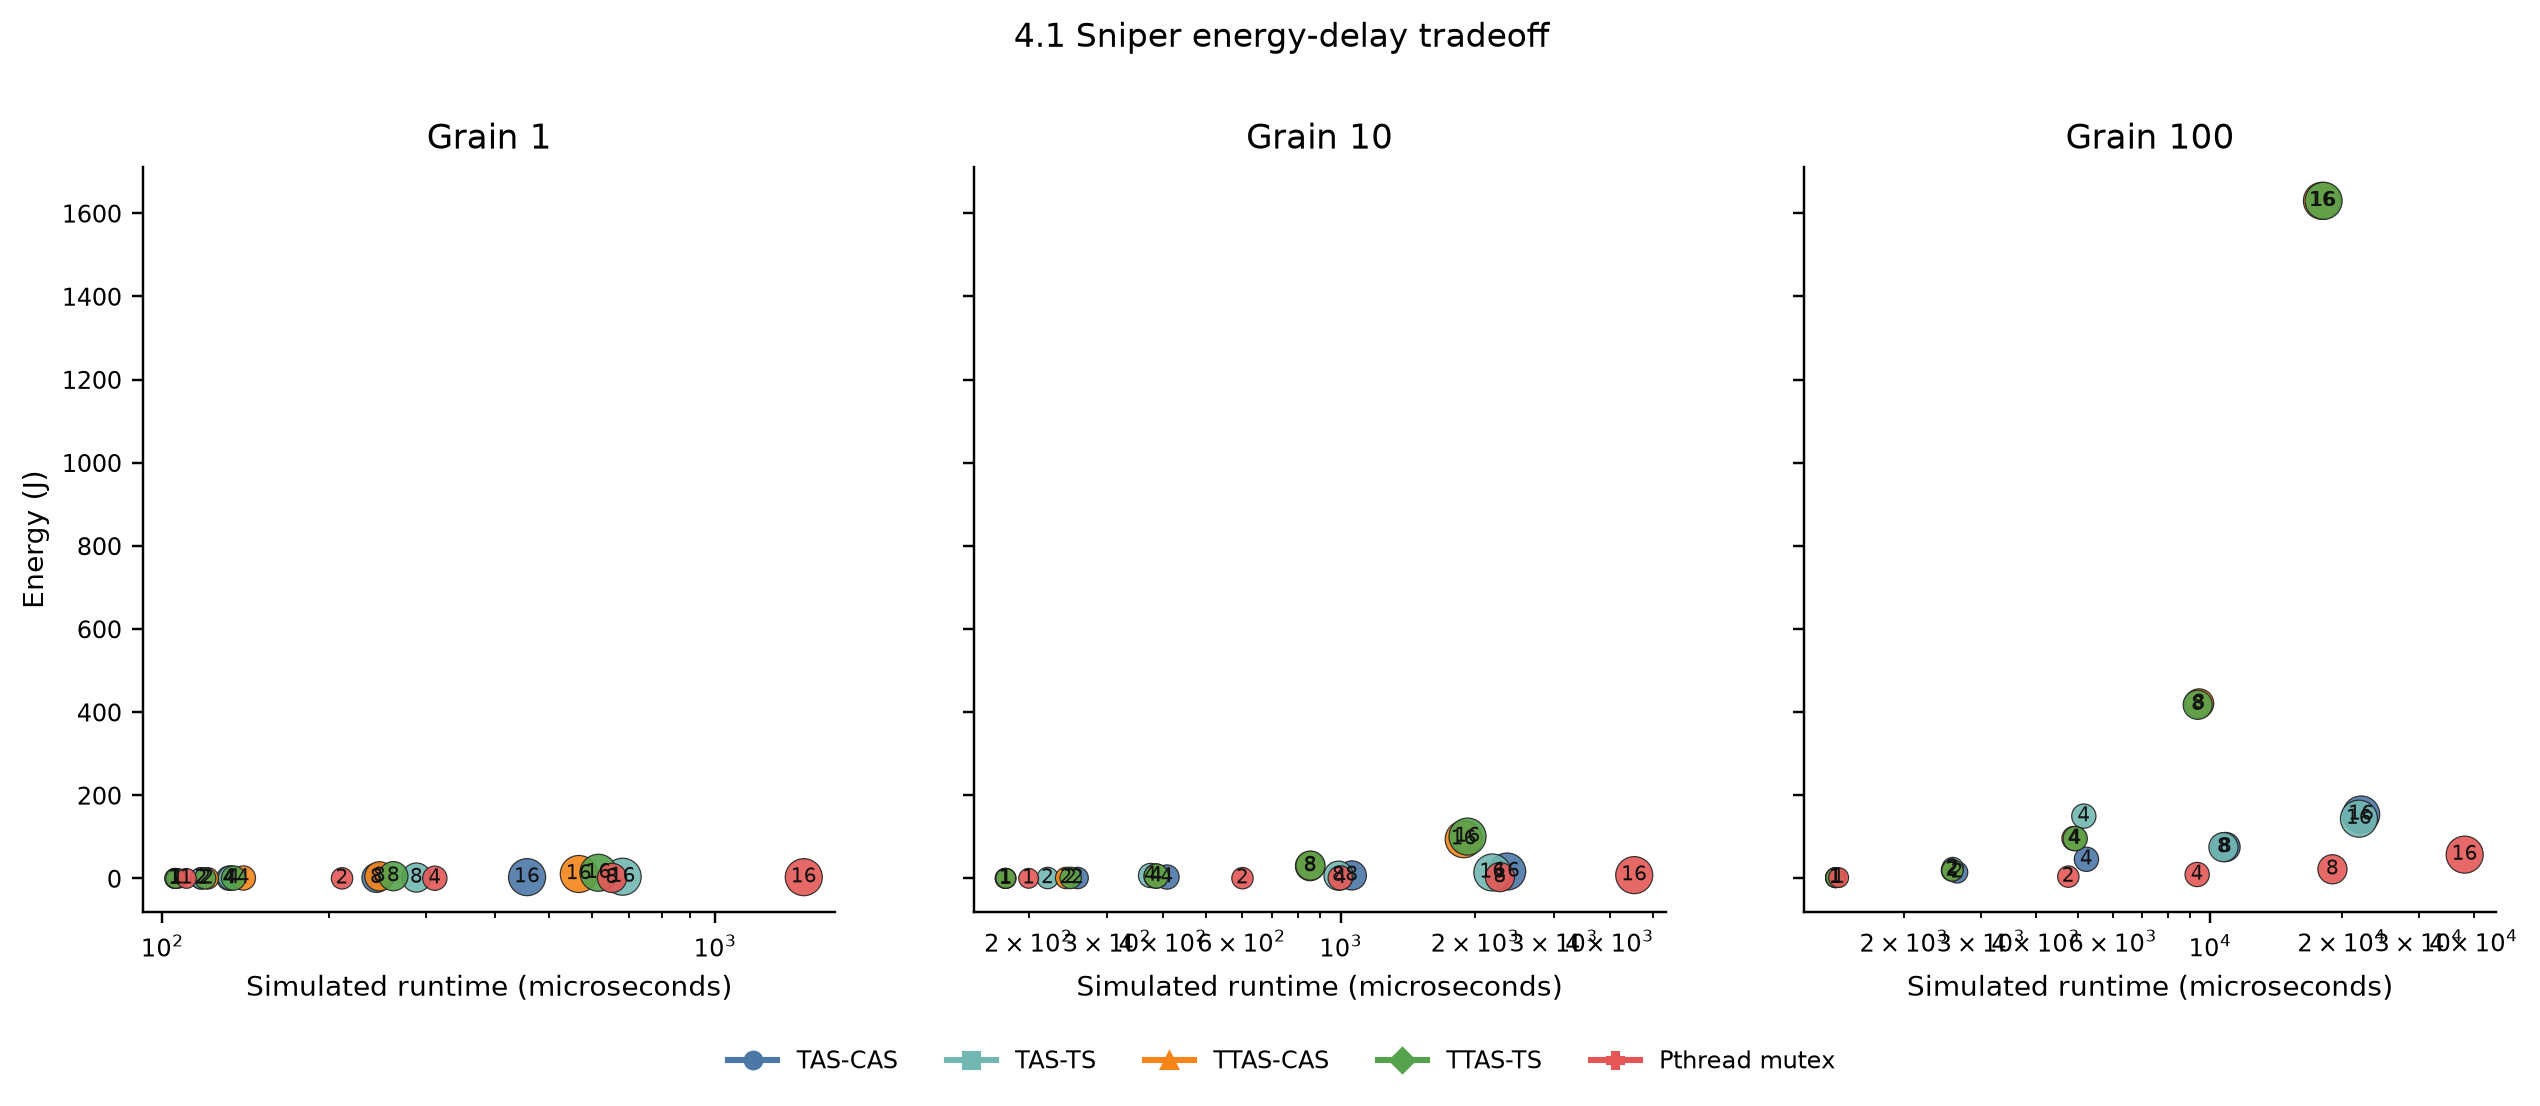
\includegraphics[width=0.84\textwidth]{4_1_sniper_energy_delay_tradeoff.png}
\caption{Σχέση χρόνου εκτέλεσης και ενέργειας για τις προσομοιώσεις Sniper.}
\label{fig:sniper-energy-delay-tradeoff}
\end{figure}

Το Διάγραμμα~\ref{fig:sniper-energy-delay-tradeoff} επιβεβαιώνει ότι δεν υπάρχει μία υλοποίηση που να είναι καθολικά βέλτιστη. Οι εκδόσεις TAS, ειδικά η \code{TAS_CAS} και η \code{TAS_TS}, παραμένουν συχνά πιο κοντά στην περιοχή χαμηλής ενέργειας. Οι εκδόσεις TTAS μετακινούνται προς μικρότερο χρόνο σε περιπτώσεις έντονου contention και μεγάλου grain, αλλά ταυτόχρονα μετακινούνται σε περιοχή υψηλότερης ενέργειας. Η \code{MUTEX} έχει χαμηλότερη ενέργεια σε ορισμένες περιπτώσεις μεγάλου grain, αλλά σημαντικά μεγαλύτερο χρόνο εκτέλεσης, ειδικά όταν αυξάνεται το πλήθος των νημάτων.

\subsection{Συγκριτική ερμηνεία των υλοποιήσεων}

Με βάση τα αποτελέσματα του Sniper, προκύπτουν οι εξής παρατηρήσεις:

\begin{itemize}
\item Για \textbf{ένα νήμα}, όλες οι υλοποιήσεις spinlock έχουν πολύ κοντινή συμπεριφορά. Αυτό είναι αναμενόμενο, επειδή δεν υπάρχει ανταγωνισμός για το lock. Οι διαφορές προκύπτουν κυρίως από το κόστος του αντίστοιχου atomic primitive και από το μήκος του κώδικα.


\item Για \textbf{μικρή τιμή grain}, η \code{TAS\_CAS} είναι η καλύτερη επιλογή ως προς τους κύκλους στα περισσότερα πλήθη νημάτων. Η TTAS λογική δεν προλαβαίνει να αξιοποιήσει το πλεονέκτημά της, επειδή η κρίσιμη περιοχή είναι πολύ μικρή και η επιπλέον διαδρομή polling επιβαρύνει την εκτέλεση.

\item Για \textbf{μεσαίο grain}, η \code{TAS\_TS} αποδίδει πολύ καλά στα λίγα νήματα, ενώ οι εκδόσεις TTAS γίνονται ταχύτερες σε \(8\) και \(16\) νήματα. Αυτό δείχνει ότι το TTAS αποκτά νόημα όταν το contention είναι αρκετό ώστε η συμπεριφορά spin-on-read να μειώνει πραγματικά τις ακριβές ατομικές προσβάσεις.

\item Για \textbf{μεγάλο grain}, οι εκδόσεις TTAS έχουν τους μικρότερους κύκλους στα περισσότερα πολυνηματικά σενάρια. Όμως, η ενεργειακή τους συμπεριφορά είναι χειρότερη, επειδή ο αριθμός των εντολών αυξάνεται δραματικά.

\item Η υλοποίηση \code{MUTEX} είναι γενικά η πιο αργή σε κύκλους στο περιβάλλον Sniper. Αυτό οφείλεται στο υψηλότερο overhead της διαδρομής του mutex της Pthreads σε σχέση με τα απλά user-level spinlocks. Ωστόσο, σε ενεργειακούς όρους δεν είναι πάντα η χειρότερη, επειδή δεν παράγει το ίδιο είδος συνεχούς δραστηριότητας εντολών ενεργού αναμονής με τις εκδόσεις TTAS.


\end{itemize}

Η βασική αρχιτεκτονική εξήγηση είναι ότι τα spinlocks δεν επιβαρύνουν μόνο τον πυρήνα που τα εκτελεί, αλλά και την ιεραρχία μνήμης. Οι εκδόσεις TAS παράγουν περισσότερες ατομικές προσπάθειες write-intent στη cache line του lock, άρα επιβαρύνουν περισσότερο το coherence protocol. Οι εκδόσεις TTAS μειώνουν αυτό το είδος traffic, επειδή οι πυρήνες που περιμένουν κάνουν απλές αναγνώσεις όσο το lock είναι κατειλημμένο. Όμως, αυτές οι αναγνώσεις εκτελούνται συνεχώς και αυξάνουν σημαντικά το πλήθος εντολών, γεγονός που φαίνεται στην ενέργεια.

Συνεπώς, από τα πειράματα Sniper προκύπτει ότι η επιλογή μηχανισμού συγχρονισμού εξαρτάται από τον στόχο βελτιστοποίησης. Αν ο στόχος είναι αποκλειστικά ο μικρότερος χρόνος εκτέλεσης σε υψηλό contention και μεγάλη κρίσιμη περιοχή, οι εκδόσεις TTAS είναι συχνά καλύτερες. Αν όμως συνεκτιμηθεί η ενέργεια ή το $EDP$, οι εκδόσεις TAS, και ιδιαίτερα η \code{TAS_TS} ή η \code{TAS_CAS} ανά περίπτωση, γίνονται πιο ελκυστικές.

\FloatBarrier

\section{Αποτελέσματα στο Πραγματικό Σύστημα}

\subsection{Συνολική εικόνα}

Στην ενότητα αυτή παρουσιάζονται τα αποτελέσματα της ίδιας πειραματικής μήτρας στο πραγματικό σύστημα. Σε αντίθεση με τον Sniper, όπου το περιβάλλον είναι ελεγχόμενο και ντετερμινιστικό, οι πραγματικές εκτελέσεις επηρεάζονται από περισσότερους παράγοντες: τον scheduler του λειτουργικού συστήματος, το περιβάλλον WSL, τη δυναμική μεταβολή συχνότητας, την υβριδική τοπολογία του επεξεργαστή, τη θερμική συμπεριφορά του laptop και τις πραγματικές υλοποιήσεις των atomic instructions και του mutex της Pthreads.

Γι' αυτό, κάθε περίπτωση εκτελέστηκε πέντε φορές και στους πίνακες αναφέρεται κυρίως η διάμεσος τιμή. Η διάμεσος είναι καταλληλότερη από τον απλό μέσο όρο όταν υπάρχουν ακραίες τιμές λόγω παροδικών παρεμβολών scheduling ή θερμικών και συχνοτικών επιδράσεων.

\subsection{Χρόνοι εκτέλεσης για \code{grain=1}}

Η περίπτωση \code{grain=1} είναι η περίπτωση με το μεγαλύτερο σχετικό κόστος συγχρονισμού. Το χρήσιμο έργο μέσα στην κρίσιμη περιοχή είναι ελάχιστο, άρα οι διαφορές μεταξύ των locks οφείλονται κυρίως στο κόστος του μηχανισμού συγχρονισμού.

\begin{figure}[htbp]
\centering
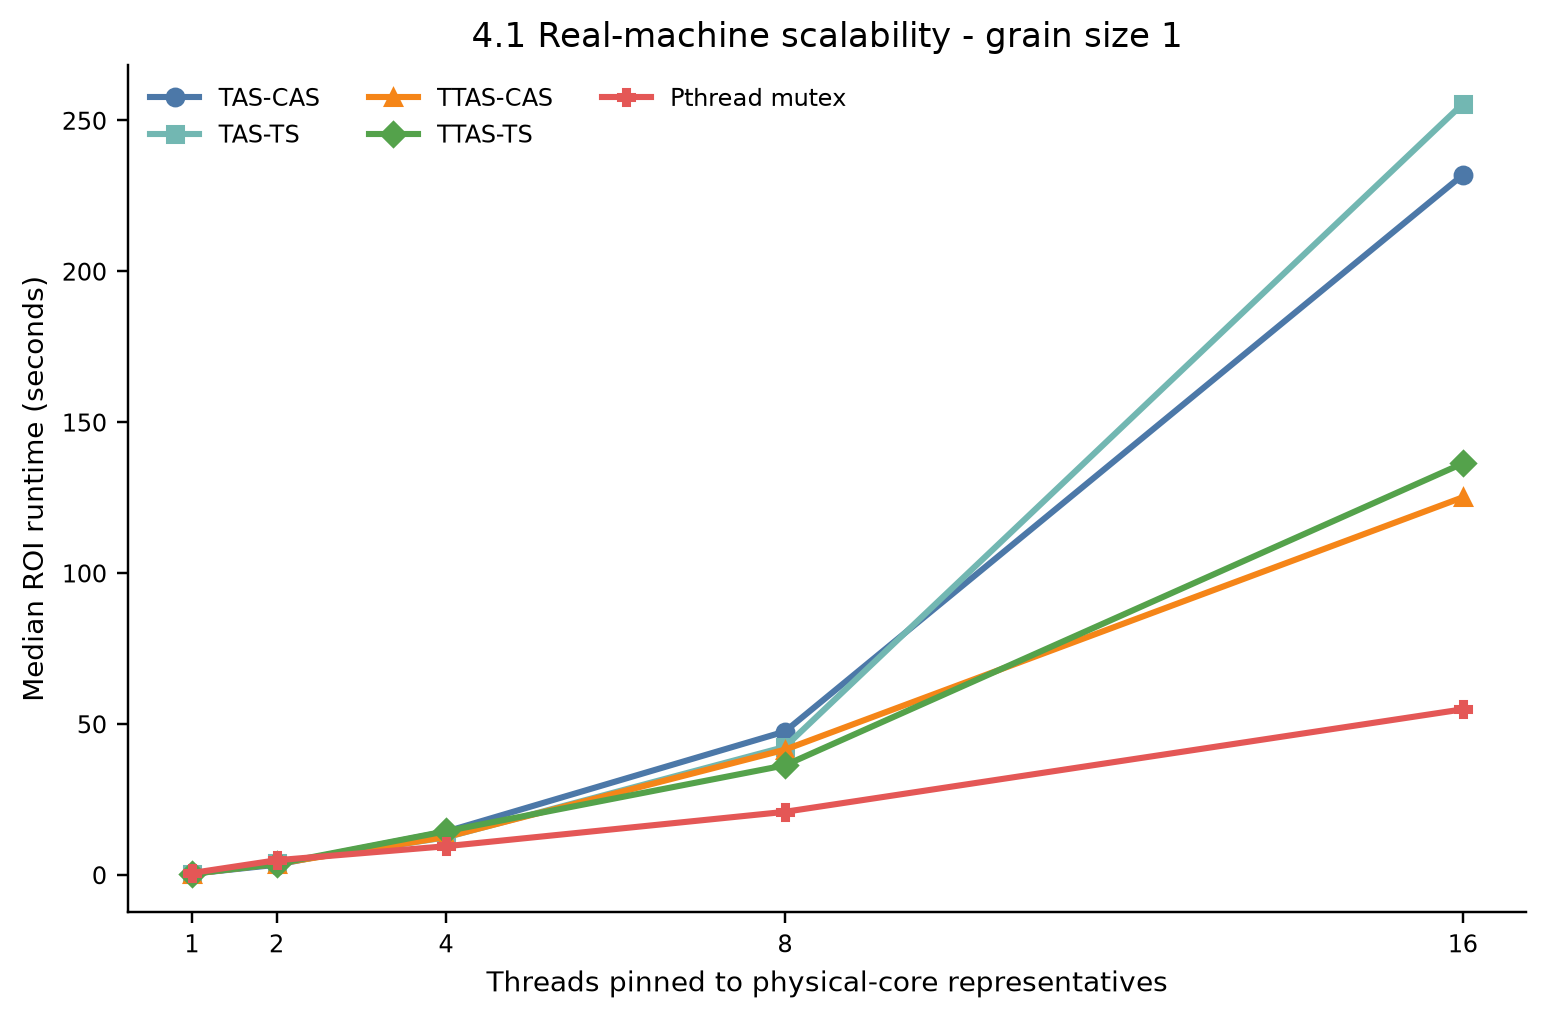
\includegraphics[width=0.82\textwidth]{4_1_real_runtime_grain_1.png}
\caption{Πραγματικός χρόνος εκτέλεσης για \code{grain=1}.}
\label{fig:real-runtime-grain-1}
\end{figure}

Στο Διάγραμμα~\ref{fig:real-runtime-grain-1} φαίνεται ότι για ένα νήμα οι υλοποιήσεις spinlock είναι σαφώς ταχύτερες από το \code{MUTEX}, αφού δεν υπάρχει πραγματικός ανταγωνισμός για το lock. Για παράδειγμα, η \code{TTAS_TS} έχει διάμεσο χρόνο \(0.365560\,\mathrm{s}\), ενώ το \code{MUTEX} έχει \(0.625282\,\mathrm{s}\). Η διαφορά αυτή οφείλεται στο μικρότερο overhead της διαδρομής user-level spinlock σε σχέση με το mutex της Pthreads.

Όταν όμως αυξάνεται το πλήθος των νημάτων, η κατάταξη αλλάζει. Για 4, 8 και 16 νήματα, το \code{MUTEX} είναι σημαντικά ταχύτερο από όλες τις εκδόσεις spinlock. Στα 16 νήματα, το \code{MUTEX} έχει διάμεσο χρόνο \(54.877071\,\mathrm{s}\), ενώ η καλύτερη εκδοχή spinlock είναι η \code{TTAS_CAS} με \(125.120595\,\mathrm{s}\). Οι εκδόσεις TAS είναι ακόμη χειρότερες, φτάνοντας τα \(231.940666\,\mathrm{s}\) και \(255.509693\,\mathrm{s}\).

Η τάση αυτή είναι χαρακτηριστική πραγματικού συστήματος: τα απλά spinlocks καταναλώνουν συνεχώς κύκλους CPU όσο περιμένουν, επιβαρύνουν την cache line του lock και παράγουν έντονο coherence traffic. Αντίθετα, το mutex της Pthreads μπορεί να αξιοποιεί μηχανισμούς blocking ή υβριδικές πολιτικές αναμονής, μειώνοντας την ενεργό σπατάλη πόρων υπό έντονο contention.

\subsection{Χρόνοι εκτέλεσης για \code{grain=10}}

Για \code{grain=10}, η κρίσιμη περιοχή έχει μεγαλύτερη διάρκεια και οι υλοποιήσεις TTAS αρχίζουν να αξιοποιούν καλύτερα το πλεονέκτημά τους, δηλαδή την αναμονή με απλές αναγνώσεις πριν από την ατομική προσπάθεια απόκτησης του lock.

\begin{figure}[htbp]
\centering
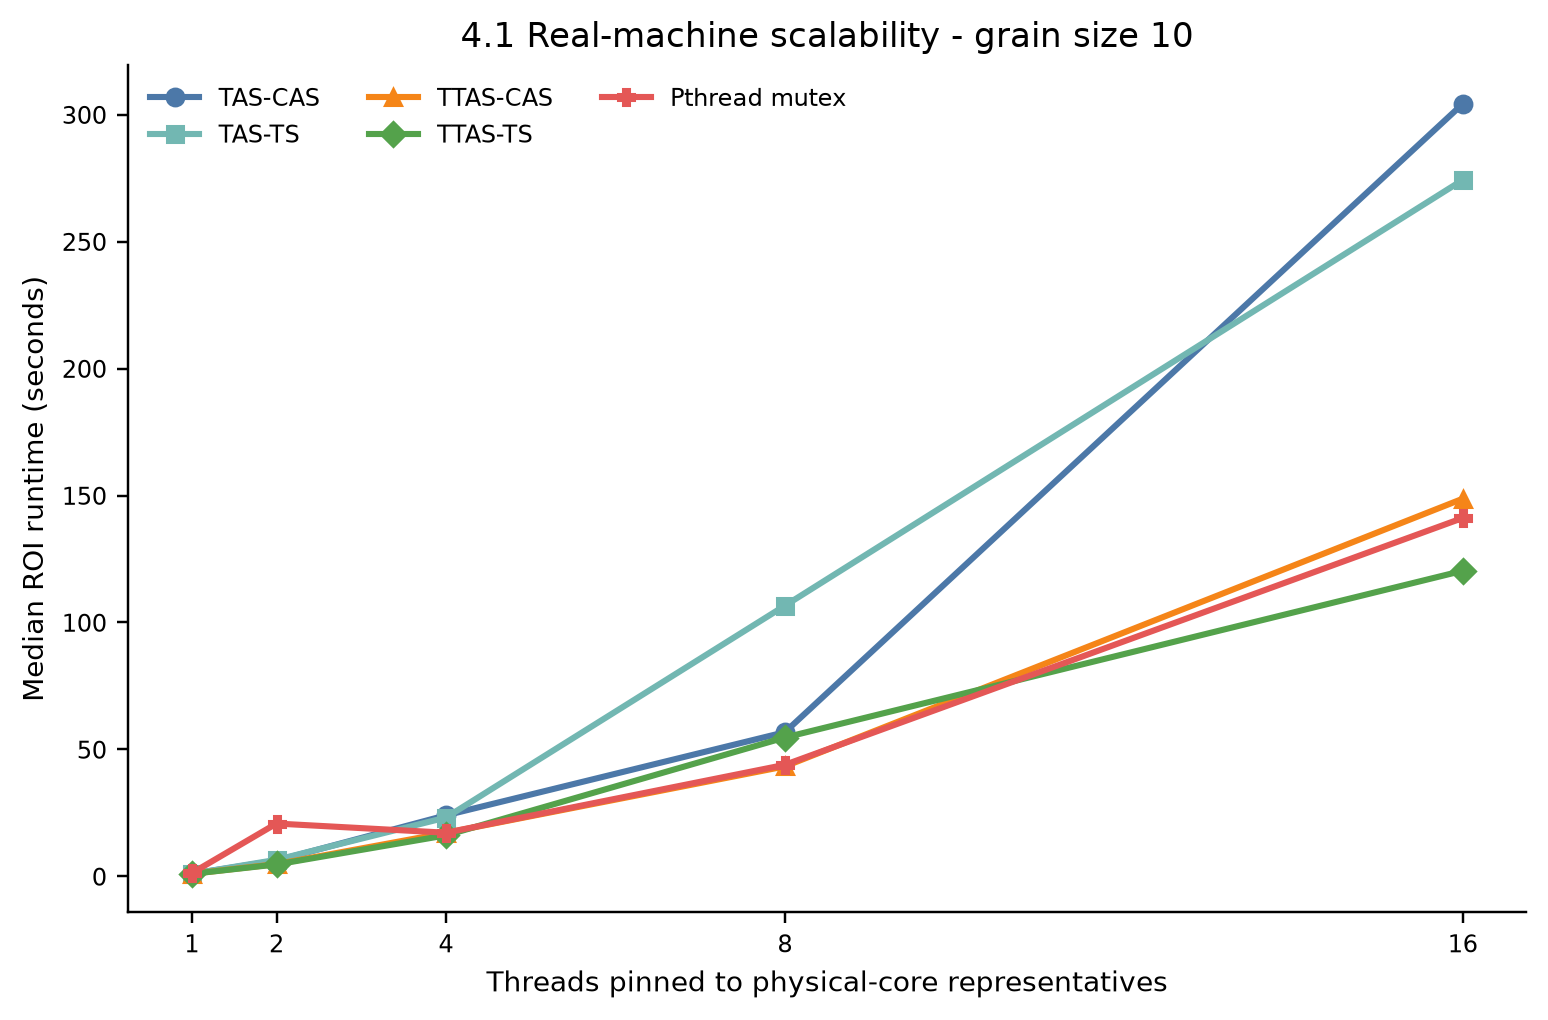
\includegraphics[width=0.82\textwidth]{4_1_real_runtime_grain_10.png}
\caption{Πραγματικός χρόνος εκτέλεσης για \code{grain=10}.}
\label{fig:real-runtime-grain-10}
\end{figure}

Στο Διάγραμμα~\ref{fig:real-runtime-grain-10}, για δύο νήματα η \code{TTAS_TS} έχει διάμεσο χρόνο \(4.701995\,\mathrm{s}\), ενώ η \code{TAS_CAS} έχει \(6.228027\,\mathrm{s}\), η \code{TAS_TS} \(6.526127\,\mathrm{s}\) και το \code{MUTEX} \(20.814586\,\mathrm{s}\). Η διαφορά είναι μεγάλη και δείχνει ότι με μέτριο grain το κόστος blocking του mutex μπορεί να γίνει μεγαλύτερο από το κόστος ενεργού spinning των TTAS.

Για 4 νήματα, η \code{TTAS_TS} παραμένει η καλύτερη με \(16.164193\,\mathrm{s}\), πολύ κοντά στην \code{TTAS_CAS} και στο \code{MUTEX}. Για 8 νήματα, η \code{TTAS_CAS} είναι οριακά καλύτερη από το \code{MUTEX}, με \(43.315459\,\mathrm{s}\) έναντι \(43.940190\,\mathrm{s}\). Για 16 νήματα, η \code{TTAS_TS} έχει την καλύτερη διάμεση τιμή, \(120.354807\,\mathrm{s}\), έναντι \(141.142824\,\mathrm{s}\) του \code{MUTEX}.

Άρα, στο πραγματικό σύστημα, η αύξηση της τιμής grain μετακινεί το βέλτιστο από το mutex της Pthreads προς τις υλοποιήσεις TTAS. Η τάση αυτή είναι συνεπής με τη θεωρία: όσο η κρίσιμη περιοχή κρατά το lock για περισσότερο χρόνο, τόσο πιο σημαντικό γίνεται τα νήματα που περιμένουν να μη δημιουργούν συνεχείς ατομικές εγγραφές.

\subsection{Χρόνοι εκτέλεσης για \code{grain=100}}

Για \code{grain=100}, το μεγαλύτερο μέρος του χρόνου αναλώνεται στην ίδια την προστατευμένη εργασία. Το contention εξακολουθεί να υπάρχει, επειδή όλα τα νήματα διεκδικούν την ίδια κρίσιμη περιοχή, αλλά το κόστος του acquire/release επιμερίζεται σε μεγαλύτερο υπολογιστικό έργο.

\begin{figure}[htbp]
\centering
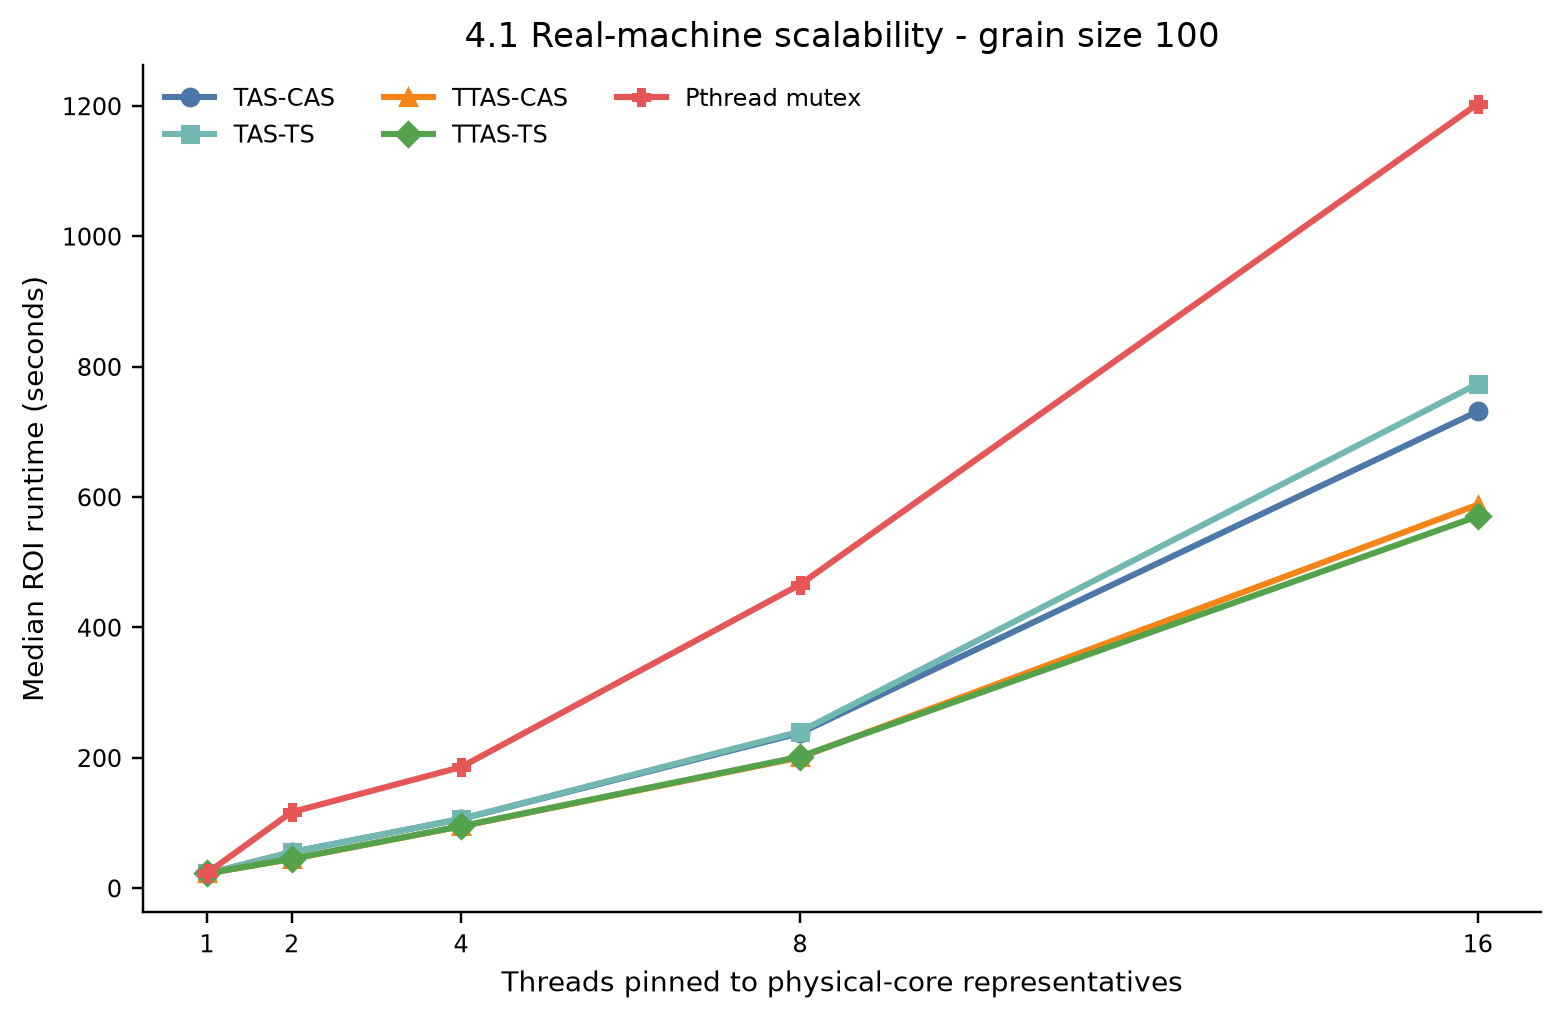
\includegraphics[width=0.82\textwidth]{4_1_real_runtime_grain_100.png}
\caption{Πραγματικός χρόνος εκτέλεσης για \code{grain=100}.}
\label{fig:real-runtime-grain-100}
\end{figure}

Στο Διάγραμμα~\ref{fig:real-runtime-grain-100}, οι υλοποιήσεις TTAS είναι πλέον οι καλύτερες σχεδόν σε όλα τα πολυνηματικά σενάρια. Για 2 νήματα, η \code{TTAS_CAS} έχει διάμεσο χρόνο \(44.590089\,\mathrm{s}\), ενώ η \code{TAS_TS} έχει \(54.961247\,\mathrm{s}\) και το \code{MUTEX} \(116.513242\,\mathrm{s}\). Για 8 νήματα, η \code{TTAS_CAS} έχει \(200.494926\,\mathrm{s}\), έναντι \(237.805654\,\mathrm{s}\) της \code{TAS_CAS} και \(465.637203\,\mathrm{s}\) του \code{MUTEX}. Για 16 νήματα, η \code{TTAS_TS} είναι η καλύτερη με \(570.500085\,\mathrm{s}\).

Το αποτέλεσμα αυτό επιβεβαιώνει ότι το TTAS είναι πιο κατάλληλο όταν υπάρχει αρκετά μεγάλη διάρκεια αναμονής. Τα νήματα που περιμένουν διαβάζουν τη μεταβλητή lock χωρίς να τη διεκδικούν ατομικά σε κάθε κύκλο αναμονής, με αποτέλεσμα να μειώνεται το coherence pressure σε σχέση με το TAS.

\subsection{Πλήρη αριθμητικά αποτελέσματα πραγματικού συστήματος}

Οι Πίνακες~\ref{tab:real-full-grain-1}, \ref{tab:real-full-grain-10} και \ref{tab:real-full-grain-100} περιέχουν τα πλήρη συγκεντρωτικά αποτελέσματα των πραγματικών εκτελέσεων. Για κάθε περίπτωση δίνονται η διάμεσος, ο μέσος όρος, η ελάχιστη, η μέγιστη και η τυπική απόκλιση των πέντε εκτελέσεων.

\begin{table}[htbp]
\centering
\scriptsize
\caption{Πλήρη πραγματικά αποτελέσματα για \code{grain=1}.}
\label{tab:real-full-grain-1}
\resizebox{\textwidth}{!}{
\begin{tabular}{P{2.4cm} P{1.4cm} P{2.2cm} P{2.2cm} P{2.2cm} P{2.2cm} P{2.2cm}}
\toprule
\textbf{Υλοποίηση} & \textbf{Νήματα} & \textbf{Διάμεσος (s)} & \textbf{Μέσος (s)} & \textbf{Ελάχιστο (s)} & \textbf{Μέγιστο (s)} & \textbf{Τυπ. απόκλιση (s)} \\
\midrule
\code{MUTEX} & 1 & 0.625282 & 0.625352 & 0.619223 & 0.631213 & 0.004264 \\
\code{TAS_CAS} & 1 & 0.388580 & 0.389946 & 0.386149 & 0.393923 & 0.003200 \\
\code{TAS_TS} & 1 & 0.365641 & 0.365552 & 0.363519 & 0.367187 & 0.001413 \\
\code{TTAS_CAS} & 1 & 0.387483 & 0.389179 & 0.384452 & 0.394591 & 0.004340 \\
\code{TTAS_TS} & 1 & 0.365560 & 0.365932 & 0.362871 & 0.369583 & 0.002673 \\
\midrule
\code{MUTEX} & 2 & 4.867422 & 4.833350 & 4.461205 & 5.059704 & 0.230307 \\
\code{TAS_CAS} & 2 & 3.383568 & 3.253162 & 2.539900 & 3.516331 & 0.402562 \\
\code{TAS_TS} & 2 & 3.857002 & 3.856281 & 3.761554 & 3.920760 & 0.059307 \\
\code{TTAS_CAS} & 2 & 3.715363 & 3.696686 & 3.434644 & 3.860722 & 0.166939 \\
\code{TTAS_TS} & 2 & 3.649147 & 3.594253 & 3.202442 & 3.935597 & 0.336343 \\
\midrule
\code{MUTEX} & 4 & 9.514252 & 9.507185 & 9.352892 & 9.679099 & 0.145902 \\
\code{TAS_CAS} & 4 & 14.353204 & 14.513917 & 13.921539 & 15.379267 & 0.614444 \\
\code{TAS_TS} & 4 & 12.454978 & 13.183069 & 11.532379 & 16.330961 & 1.866334 \\
\code{TTAS_CAS} & 4 & 12.571901 & 12.835737 & 12.367053 & 14.074234 & 0.698570 \\
\code{TTAS_TS} & 4 & 14.483348 & 13.894314 & 12.267918 & 14.595089 & 1.003549 \\
\midrule
\code{MUTEX} & 8 & 20.908853 & 20.807249 & 19.010152 & 22.291668 & 1.170593 \\
\code{TAS_CAS} & 8 & 47.523549 & 46.763366 & 40.732706 & 55.142507 & 5.789792 \\
\code{TAS_TS} & 8 & 42.430114 & 43.952958 & 36.185565 & 53.704676 & 7.689683 \\
\code{TTAS_CAS} & 8 & 41.502087 & 39.545699 & 33.119133 & 43.979758 & 4.650920 \\
\code{TTAS_TS} & 8 & 36.316803 & 37.106070 & 33.591975 & 41.357436 & 3.471241 \\
\midrule
\code{MUTEX} & 16 & 54.877071 & 54.671704 & 50.281476 & 58.871284 & 3.604041 \\
\code{TAS_CAS} & 16 & 231.940666 & 239.458935 & 226.190911 & 257.127362 & 15.406106 \\
\code{TAS_TS} & 16 & 255.509693 & 241.194452 & 204.806532 & 274.306179 & 33.440446 \\
\code{TTAS_CAS} & 16 & 125.120595 & 127.560030 & 112.617907 & 141.522433 & 10.876243 \\
\code{TTAS_TS} & 16 & 136.358652 & 133.586265 & 119.602134 & 140.188683 & 8.340048 \\
\bottomrule
\end{tabular}
}
\end{table}

\begin{table}[htbp]
\centering
\scriptsize
\caption{Πλήρη πραγματικά αποτελέσματα για \code{grain=10}.}
\label{tab:real-full-grain-10}
\resizebox{\textwidth}{!}{
\begin{tabular}{P{2.4cm} P{1.4cm} P{2.2cm} P{2.2cm} P{2.2cm} P{2.2cm} P{2.2cm}}
\toprule
\textbf{Υλοποίηση} & \textbf{Νήματα} & \textbf{Διάμεσος (s)} & \textbf{Μέσος (s)} & \textbf{Ελάχιστο (s)} & \textbf{Μέγιστο (s)} & \textbf{Τυπ. απόκλιση (s)} \\
\midrule
\code{MUTEX} & 1 & 1.270058 & 1.272023 & 1.269037 & 1.276141 & 0.003518 \\
\code{TAS_CAS} & 1 & 1.022487 & 1.019707 & 1.007908 & 1.027451 & 0.007667 \\
\code{TAS_TS} & 1 & 1.013479 & 1.015765 & 1.009167 & 1.023168 & 0.006064 \\
\code{TTAS_CAS} & 1 & 1.025173 & 0.990532 & 0.859653 & 1.032387 & 0.074008 \\
\code{TTAS_TS} & 1 & 1.003555 & 1.006238 & 0.999335 & 1.019620 & 0.007835 \\
\midrule
\code{MUTEX} & 2 & 20.814586 & 20.723908 & 20.543597 & 20.846998 & 0.143508 \\
\code{TAS_CAS} & 2 & 6.228027 & 6.215498 & 5.884268 & 6.551387 & 0.241017 \\
\code{TAS_TS} & 2 & 6.526127 & 6.246859 & 5.012119 & 6.746715 & 0.716597 \\
\code{TTAS_CAS} & 2 & 4.839458 & 5.240460 & 4.599659 & 6.890670 & 0.936013 \\
\code{TTAS_TS} & 2 & 4.701995 & 5.069514 & 4.349903 & 6.679558 & 0.923082 \\
\midrule
\code{MUTEX} & 4 & 17.200449 & 17.535659 & 16.933532 & 18.307858 & 0.634744 \\
\code{TAS_CAS} & 4 & 24.048892 & 22.111317 & 18.155025 & 24.618480 & 3.076097 \\
\code{TAS_TS} & 4 & 23.164807 & 22.664123 & 20.973434 & 23.908054 & 1.293132 \\
\code{TTAS_CAS} & 4 & 17.141481 & 16.903488 & 15.578576 & 17.442104 & 0.754264 \\
\code{TTAS_TS} & 4 & 16.164193 & 16.118244 & 14.226026 & 18.303340 & 1.590734 \\
\midrule
\code{MUTEX} & 8 & 43.940190 & 43.831461 & 43.094775 & 44.260435 & 0.461705 \\
\code{TAS_CAS} & 8 & 56.783915 & 70.213067 & 55.738369 & 101.230579 & 20.479764 \\
\code{TAS_TS} & 8 & 106.616139 & 103.019439 & 86.874820 & 108.681650 & 9.182279 \\
\code{TTAS_CAS} & 8 & 43.315459 & 44.880062 & 37.790287 & 56.459905 & 7.517331 \\
\code{TTAS_TS} & 8 & 54.695458 & 52.151812 & 47.647241 & 55.065152 & 3.713082 \\
\midrule
\code{MUTEX} & 16 & 141.142824 & 141.241101 & 137.790994 & 145.078378 & 2.591613 \\
\code{TAS_CAS} & 16 & 304.248554 & 322.086918 & 286.006952 & 367.794231 & 38.501591 \\
\code{TAS_TS} & 16 & 274.279948 & 303.631606 & 273.253495 & 397.126231 & 53.417673 \\
\code{TTAS_CAS} & 16 & 148.735229 & 143.938287 & 124.170733 & 164.062258 & 18.230088 \\
\code{TTAS_TS} & 16 & 120.354807 & 130.649110 & 114.001055 & 160.337573 & 19.774261 \\
\bottomrule
\end{tabular}
}
\end{table}

\begin{table}[htbp]
\centering
\scriptsize
\caption{Πλήρη πραγματικά αποτελέσματα για \code{grain=100}.}
\label{tab:real-full-grain-100}
\resizebox{\textwidth}{!}{
\begin{tabular}{P{2.4cm} P{1.4cm} P{2.2cm} P{2.2cm} P{2.2cm} P{2.2cm} P{2.2cm}}
\toprule
\textbf{Υλοποίηση} & \textbf{Νήματα} & \textbf{Διάμεσος (s)} & \textbf{Μέσος (s)} & \textbf{Ελάχιστο (s)} & \textbf{Μέγιστο (s)} & \textbf{Τυπ. απόκλιση (s)} \\
\midrule
\code{MUTEX} & 1 & 22.801103 & 22.795303 & 22.692633 & 22.846130 & 0.062193 \\
\code{TAS_CAS} & 1 & 21.924664 & 21.939094 & 21.847293 & 22.060111 & 0.078637 \\
\code{TAS_TS} & 1 & 22.497352 & 22.471470 & 22.361320 & 22.521710 & 0.066251 \\
\code{TTAS_CAS} & 1 & 22.632367 & 22.569793 & 22.430253 & 22.643509 & 0.095226 \\
\code{TTAS_TS} & 1 & 22.483587 & 22.498071 & 22.330410 & 22.646958 & 0.136216 \\
\midrule
\code{MUTEX} & 2 & 116.513242 & 116.682895 & 116.451634 & 117.440379 & 0.425511 \\
\code{TAS_CAS} & 2 & 55.144021 & 55.119180 & 54.747143 & 55.360995 & 0.243071 \\
\code{TAS_TS} & 2 & 54.961247 & 54.898442 & 54.656769 & 55.102404 & 0.183765 \\
\code{TTAS_CAS} & 2 & 44.590089 & 44.682668 & 44.573007 & 44.923671 & 0.153640 \\
\code{TTAS_TS} & 2 & 44.933238 & 44.934464 & 44.431614 & 45.325088 & 0.328475 \\
\midrule
\code{MUTEX} & 4 & 185.676879 & 185.721897 & 184.608294 & 187.337828 & 1.043493 \\
\code{TAS_CAS} & 4 & 106.014213 & 105.884182 & 105.483608 & 106.236225 & 0.316709 \\
\code{TAS_TS} & 4 & 106.122463 & 106.250826 & 105.789289 & 106.743283 & 0.418997 \\
\code{TTAS_CAS} & 4 & 94.818556 & 94.718205 & 94.346246 & 95.063895 & 0.282683 \\
\code{TTAS_TS} & 4 & 94.946787 & 94.658973 & 94.148129 & 94.974775 & 0.416247 \\
\midrule
\code{MUTEX} & 8 & 465.637203 & 467.512796 & 456.491275 & 480.182405 & 10.980537 \\
\code{TAS_CAS} & 8 & 237.805654 & 238.225174 & 236.177803 & 241.129944 & 2.130201 \\
\code{TAS_TS} & 8 & 240.043655 & 248.886425 & 238.260444 & 282.828136 & 19.148541 \\
\code{TTAS_CAS} & 8 & 200.494926 & 200.090920 & 198.393127 & 201.299631 & 1.175322 \\
\code{TTAS_TS} & 8 & 201.551110 & 201.483626 & 200.564581 & 202.031600 & 0.614287 \\
\midrule
\code{MUTEX} & 16 & 1203.154081 & 1202.801726 & 1197.222199 & 1210.309613 & 5.111616 \\
\code{TAS_CAS} & 16 & 731.310517 & 730.241316 & 715.278046 & 745.484792 & 11.148254 \\
\code{TAS_TS} & 16 & 773.666274 & 760.214690 & 709.925601 & 786.646507 & 32.013783 \\
\code{TTAS_CAS} & 16 & 588.185865 & 596.247813 & 584.712974 & 611.428767 & 13.185827 \\
\code{TTAS_TS} & 16 & 570.500085 & 572.061813 & 557.713162 & 586.840093 & 13.689552 \\
\bottomrule
\end{tabular}
}
\end{table}

\FloatBarrier

\subsection{Μεταβλητότητα πραγματικών μετρήσεων}

Η μεταβλητότητα των πραγματικών εκτελέσεων φαίνεται στο Διάγραμμα~\ref{fig:real-runtime-variability}. Η μεταβλητότητα είναι αναμενόμενα μεγαλύτερη από αυτή των προσομοιώσεων, επειδή το πραγματικό σύστημα δεν είναι απομονωμένο ούτε πλήρως ντετερμινιστικό.

\begin{figure}[htbp]
\centering
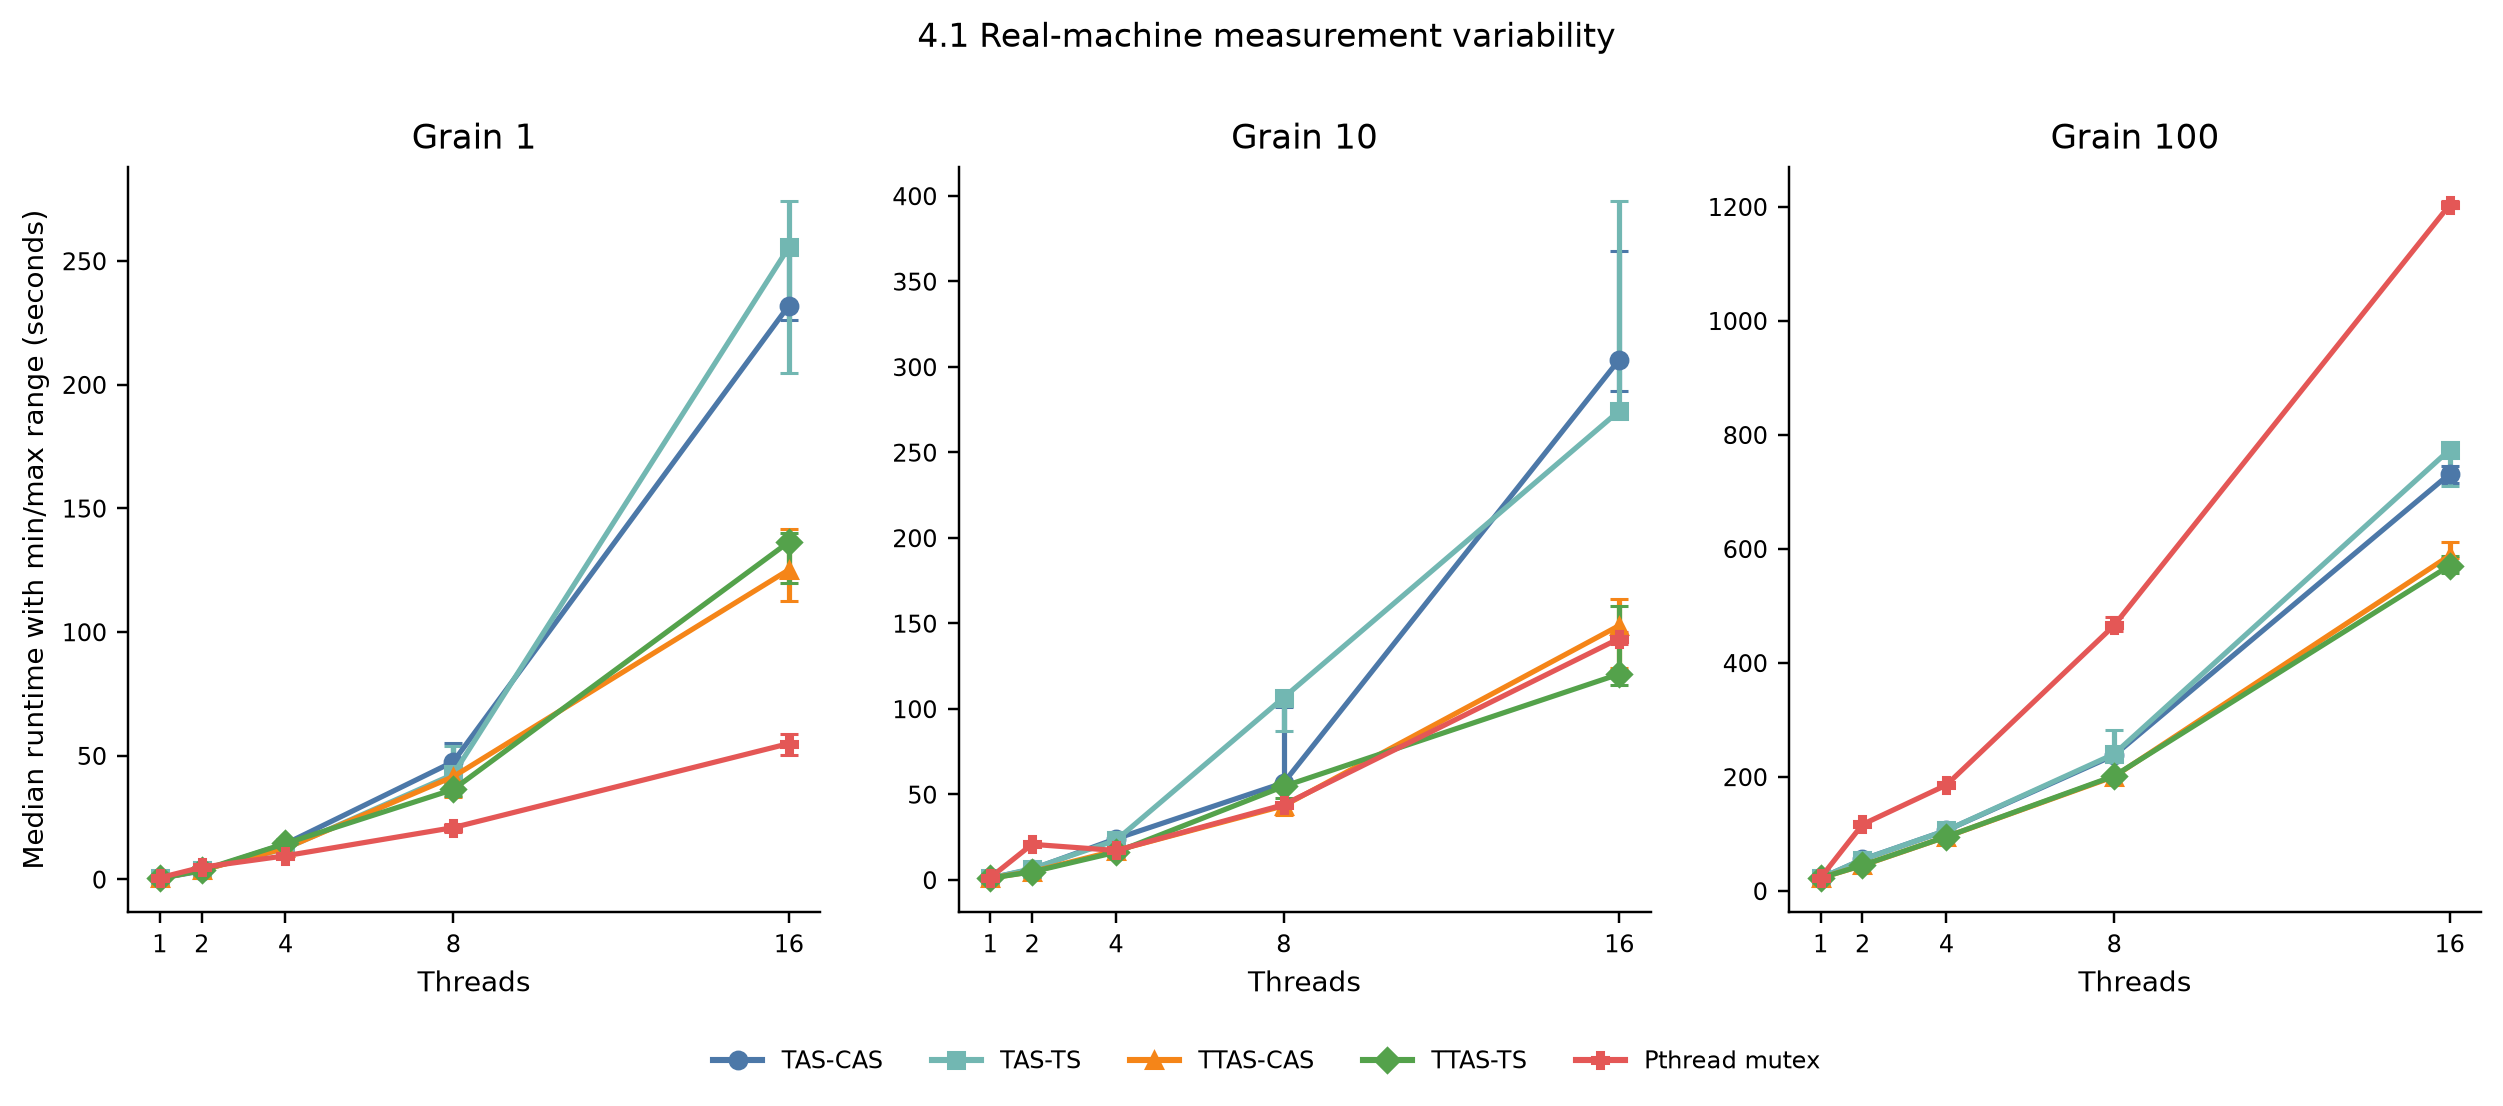
\includegraphics[width=0.86\textwidth]{4_1_real_runtime_variability.png}
\caption{Μεταβλητότητα πραγματικών χρόνων εκτέλεσης ανά υλοποίηση, νήματα και grain.}
\label{fig:real-runtime-variability}
\end{figure}

Οι μεγαλύτερες αποκλίσεις εμφανίζονται κυρίως σε πολυνηματικές εκτελέσεις spinlock, όπου το ενεργό spinning κάνει το benchmark πιο ευαίσθητο σε scheduling παρεμβολές, συχνότητα πυρήνων και θερμική κατάσταση. Για παράδειγμα, στο \code{grain=10}, η \code{TAS_CAS} στα 8 νήματα έχει διάμεσο χρόνο \(56.783915\,\mathrm{s}\), αλλά μέγιστη τιμή \(101.230579\,\mathrm{s}\), κάτι που δείχνει έντονη ακραία τιμή. Αντίστοιχα, η \code{TAS_TS} στα 16 νήματα έχει τυπική απόκλιση \(53.417673\,\mathrm{s}\). Αυτή η συμπεριφορά δικαιολογεί τη χρήση της διαμέσου ως κύριας μετρικής.

\subsection{Σύγκριση Sniper και πραγματικού συστήματος}

Η σύγκριση Sniper και πραγματικού συστήματος δεν πρέπει να ερμηνευθεί ως απόλυτη σύγκριση χρόνων, επειδή πρόκειται για διαφορετικά περιβάλλοντα. Ο Sniper μοντελοποιεί συγκεκριμένη αρχιτεκτονική με σταθερή συχνότητα και συγκεκριμένη ιεραρχία της cache. Το πραγματικό σύστημα είναι υβριδικό Intel laptop CPU, εκτελείται μέσω WSL και υπόκειται σε OS scheduling και δυναμικές πολιτικές ισχύος.

Γι' αυτό, η σύγκριση γίνεται κυρίως σε επίπεδο τάσεων. Το Διάγραμμα~\ref{fig:sniper-vs-real-normalized} δείχνει κανονικοποιημένη συμπεριφορά κλιμάκωσης.

\begin{figure}[htbp]
\centering
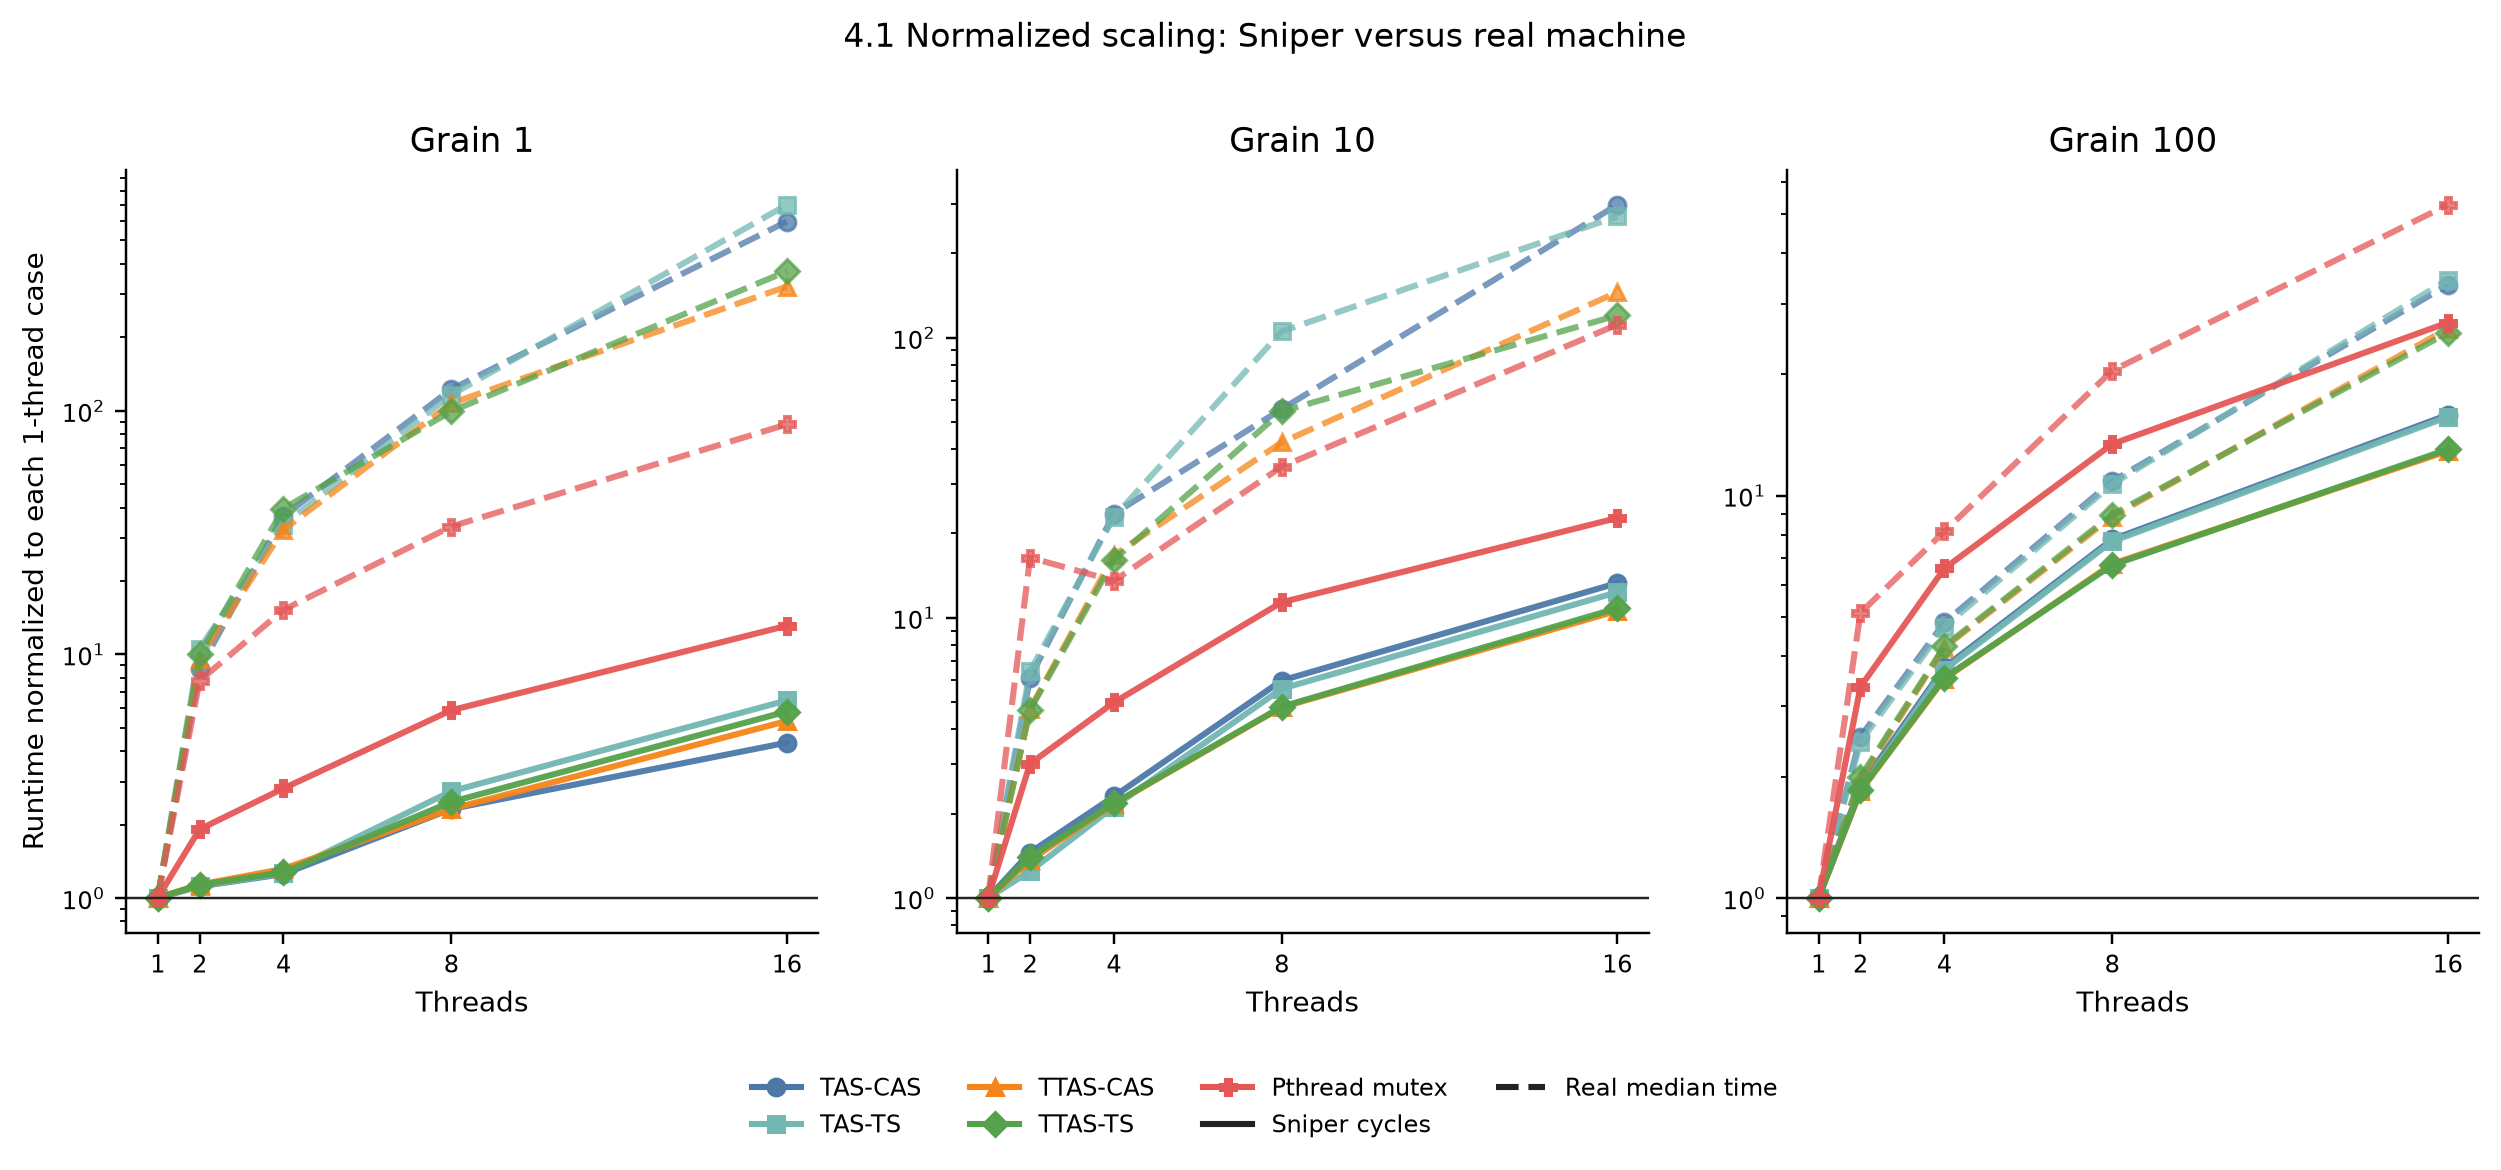
\includegraphics[width=0.86\textwidth]{4_1_sniper_vs_real_normalized_scaling.png}
\caption{Κανονικοποιημένη σύγκριση κλιμάκωσης Sniper και πραγματικού συστήματος.}
\label{fig:sniper-vs-real-normalized}
\end{figure}

Η βασική διαφορά είναι ότι στον Sniper οι απλές υλοποιήσεις spinlock, ιδιαίτερα η \code{TAS_CAS} και η \code{TAS_TS}, δίνουν συχνά ανταγωνιστικό πλήθος κύκλων, ενώ στο πραγματικό σύστημα το \code{MUTEX} είναι πολύ καλύτερο στο \code{grain=1} και οι υλοποιήσεις TTAS είναι καλύτερες στις μεγαλύτερες τιμές grain. Η διαφορά αυτή οφείλεται κυρίως σε τρεις παράγοντες.

Πρώτον, η πραγματική υλοποίηση του mutex της Pthreads είναι ιδιαίτερα βελτιστοποιημένη και μπορεί να αποφύγει μέρος της ενεργής αναμονής όταν το lock έχει υψηλό contention. Δεύτερον, τα απλά spinlocks εκτελούνται συνεχώς και καταναλώνουν πραγματικούς πόρους πυρήνα, δημιουργώντας πίεση στην ιεραρχία της cache και στο υποσύστημα μνήμης. Τρίτον, το πραγματικό σύστημα είναι υβριδικό και δεν έχει την απλή, ομοιογενή τοπολογία του προσομοιωμένου συστήματος.

Παρ' όλα αυτά, υπάρχει κοινή ποιοτική τάση: όσο αυξάνεται το grain, οι υλοποιήσεις TTAS γίνονται πιο ελκυστικές ως προς τον χρόνο εκτέλεσης, επειδή μειώνουν τις άσκοπες ατομικές προσβάσεις κατά την αναμονή. Αυτή η τάση εμφανίζεται και στον Sniper και στο πραγματικό σύστημα, αν και με διαφορετικό μέγεθος επίδρασης.

\section{Πειράματα Τοπολογίας στον Sniper}

\subsection{Στόχος των πειραμάτων τοπολογίας}

Τα πειράματα της ενότητας 4.2 εξετάζουν πώς επηρεάζεται η απόδοση των locks από το επίπεδο διαμοιρασμού της ιεραρχίας της cache. Χρησιμοποιούνται 4 νήματα, 1000 επαναλήψεις και \code{grain=1}, ώστε η εκτέλεση να είναι ιδιαίτερα ευαίσθητη στο κόστος συγχρονισμού. Οι τρεις τοπολογίες είναι:

\begin{itemize}
\item \code{share-all}: κοινή L2 και κοινή L3 για τα τέσσερα νήματα.
\item \code{share-l3}: ιδιωτική L2 ανά πυρήνα, κοινή L3.
\item \code{share-nothing}: χωρίς κοινή L2 ή L3 μεταξύ των πυρήνων.
\end{itemize}

Σε επίπεδο coherence, η τοπολογία έχει άμεση σημασία επειδή η cache line του lock πρέπει να γίνεται ορατή και να μεταφέρεται μεταξύ των πυρήνων. Όσο πιο κοντά βρίσκεται το επίπεδο κοινής cache, τόσο φθηνότερη μπορεί να είναι η επικοινωνία. Αντίθετα, όταν δεν υπάρχει κοινό χαμηλό επίπεδο cache, η μεταφορά ownership και οι invalidations γίνονται ακριβότερες.

\subsection{Κύκλοι εκτέλεσης ανά τοπολογία}

\begin{figure}[htbp]
\centering
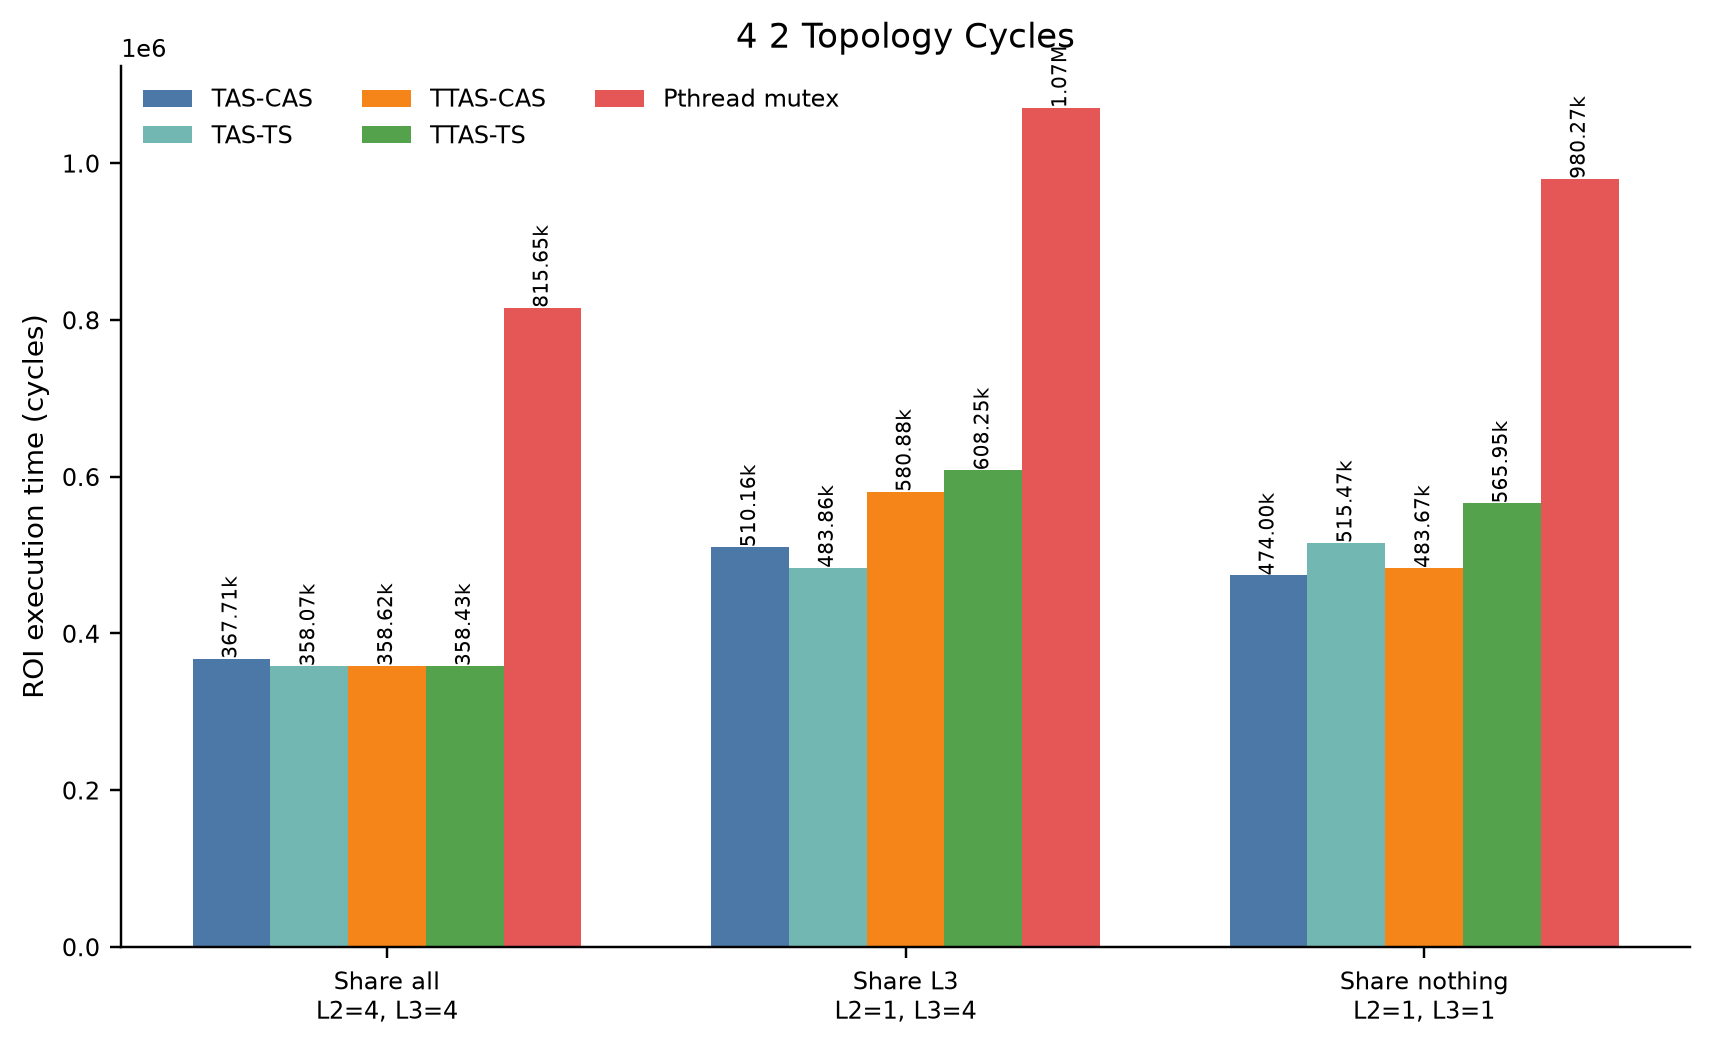
\includegraphics[width=0.82\textwidth]{4_2_topology_cycles.png}
\caption{Κύκλοι εκτέλεσης για τις τρεις τοπολογίες της ενότητας 4.2.}
\label{fig:topology-cycles}
\end{figure}

Στο Διάγραμμα~\ref{fig:topology-cycles} φαίνεται ότι η υλοποίηση \code{MUTEX} είναι η πιο αργή και στις τρεις τοπολογίες. Η διαφορά της από τα spinlocks είναι ιδιαίτερα μεγάλη στη \code{share-l3} τοπολογία, όπου απαιτεί 1{,}070{,}543 κύκλους, ενώ η καλύτερη εκδοχή spinlock, η \code{TAS_TS}, απαιτεί (483{,}855) κύκλους.

Στη \code{share-all} τοπολογία, όλες οι εκδόσεις spinlock είναι πολύ κοντά μεταξύ τους. Η \code{TAS_TS}, η \code{TTAS_CAS} και η \code{TTAS_TS} έχουν περίπου 358K κύκλους. Αυτό δείχνει ότι, όταν όλα τα νήματα μοιράζονται χαμηλό επίπεδο cache, το κόστος μετακίνησης της cache line του lock είναι μικρότερο και οι διαφορές μεταξύ των πολιτικών spinlock περιορίζονται.

Στη \code{share-l3} τοπολογία, οι υλοποιήσεις TAS έχουν καλύτερη συμπεριφορά από τις TTAS. Η \code{TAS_TS} έχει (483{,}855) κύκλους και η \code{TAS_CAS} (510{,}158), ενώ οι υλοποιήσεις TTAS έχουν (580{,}885) και (608{,}246) κύκλους. Αυτό δείχνει ότι, για μικρή τιμή grain και ιδιωτική L2, η επιπλέον διαδικασία polling των TTAS δεν οδηγεί πάντα σε καλύτερη απόδοση.

Στη \code{share-nothing} τοπολογία, η \code{TAS_CAS} είναι η ταχύτερη με (473{,}997) κύκλους, ενώ η \code{TTAS_CAS} είναι πολύ κοντά με (483{,}674). Η \code{TTAS_TS} είναι πιο αργή, με (565{,}954) κύκλους. Συνεπώς, για πολύ μικρή κρίσιμη περιοχή, η απλότητα των μηχανισμών TAS μπορεί να υπερισχύσει, ακόμη και όταν η τοπολογία κάνει την επικοινωνία ακριβότερη.

\begin{figure}[htbp]
\centering
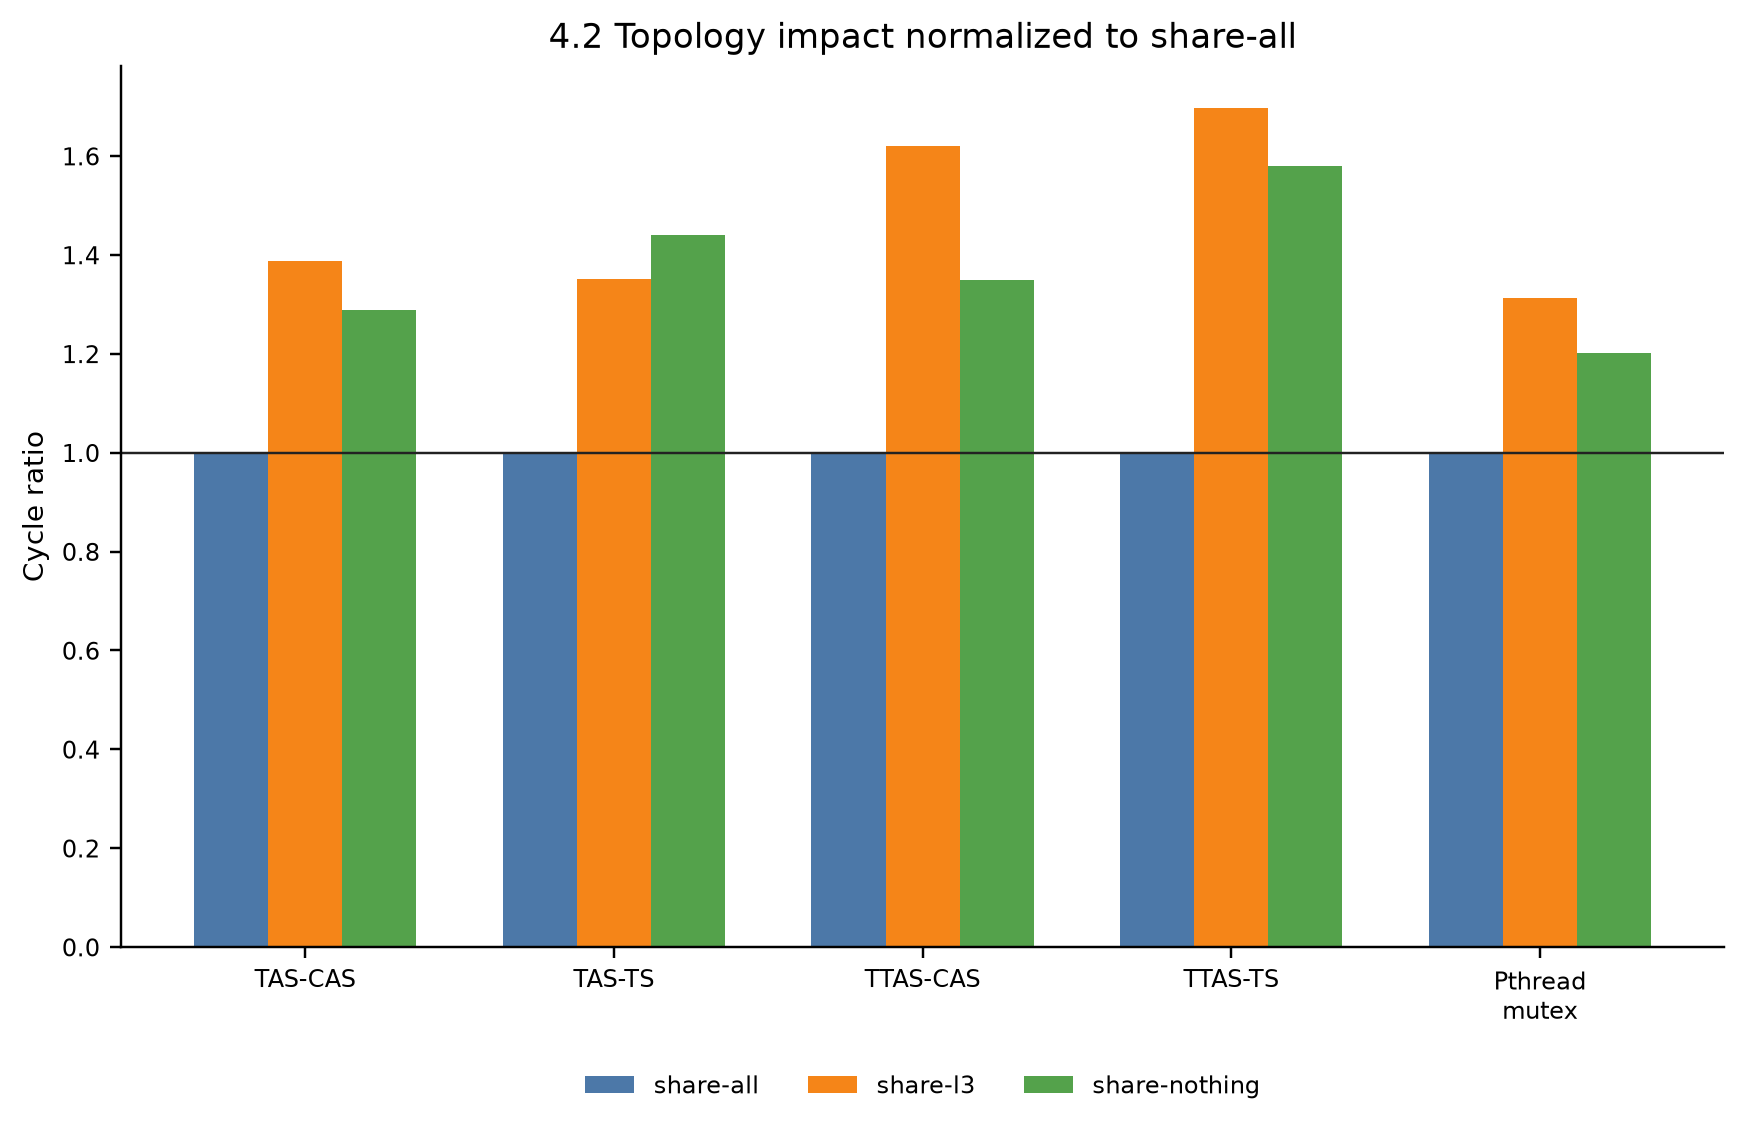
\includegraphics[width=0.82\textwidth]{4_2_topology_cycles_normalized.png}
\caption{Κανονικοποιημένοι κύκλοι εκτέλεσης ανά τοπολογία.}
\label{fig:topology-cycles-normalized}
\end{figure}

Το Διάγραμμα~\ref{fig:topology-cycles-normalized} βοηθά να φανεί η σχετική επιδείνωση κάθε υλοποίησης όταν αλλάζει η τοπολογία. Η \code{MUTEX} παρουσιάζει μεγάλη ευαισθησία, ενώ οι υλοποιήσεις spinlock έχουν πιο περιορισμένες μεταβολές, αν και όχι αμελητέες. Η \code{share-all} τοπολογία είναι γενικά η καλύτερη για τις εκδόσεις spinlock, επειδή τα νήματα μοιράζονται χαμηλότερο επίπεδο της cache.

\subsection{Ενεργειακά αποτελέσματα τοπολογίας}

Τα ενεργειακά αποτελέσματα των πειραμάτων τοπολογίας δίνονται στα Διαγράμματα~\ref{fig:topology-energy}, \ref{fig:topology-edp} και \ref{fig:topology-ed2p}.

\begin{figure}[htbp]
\centering
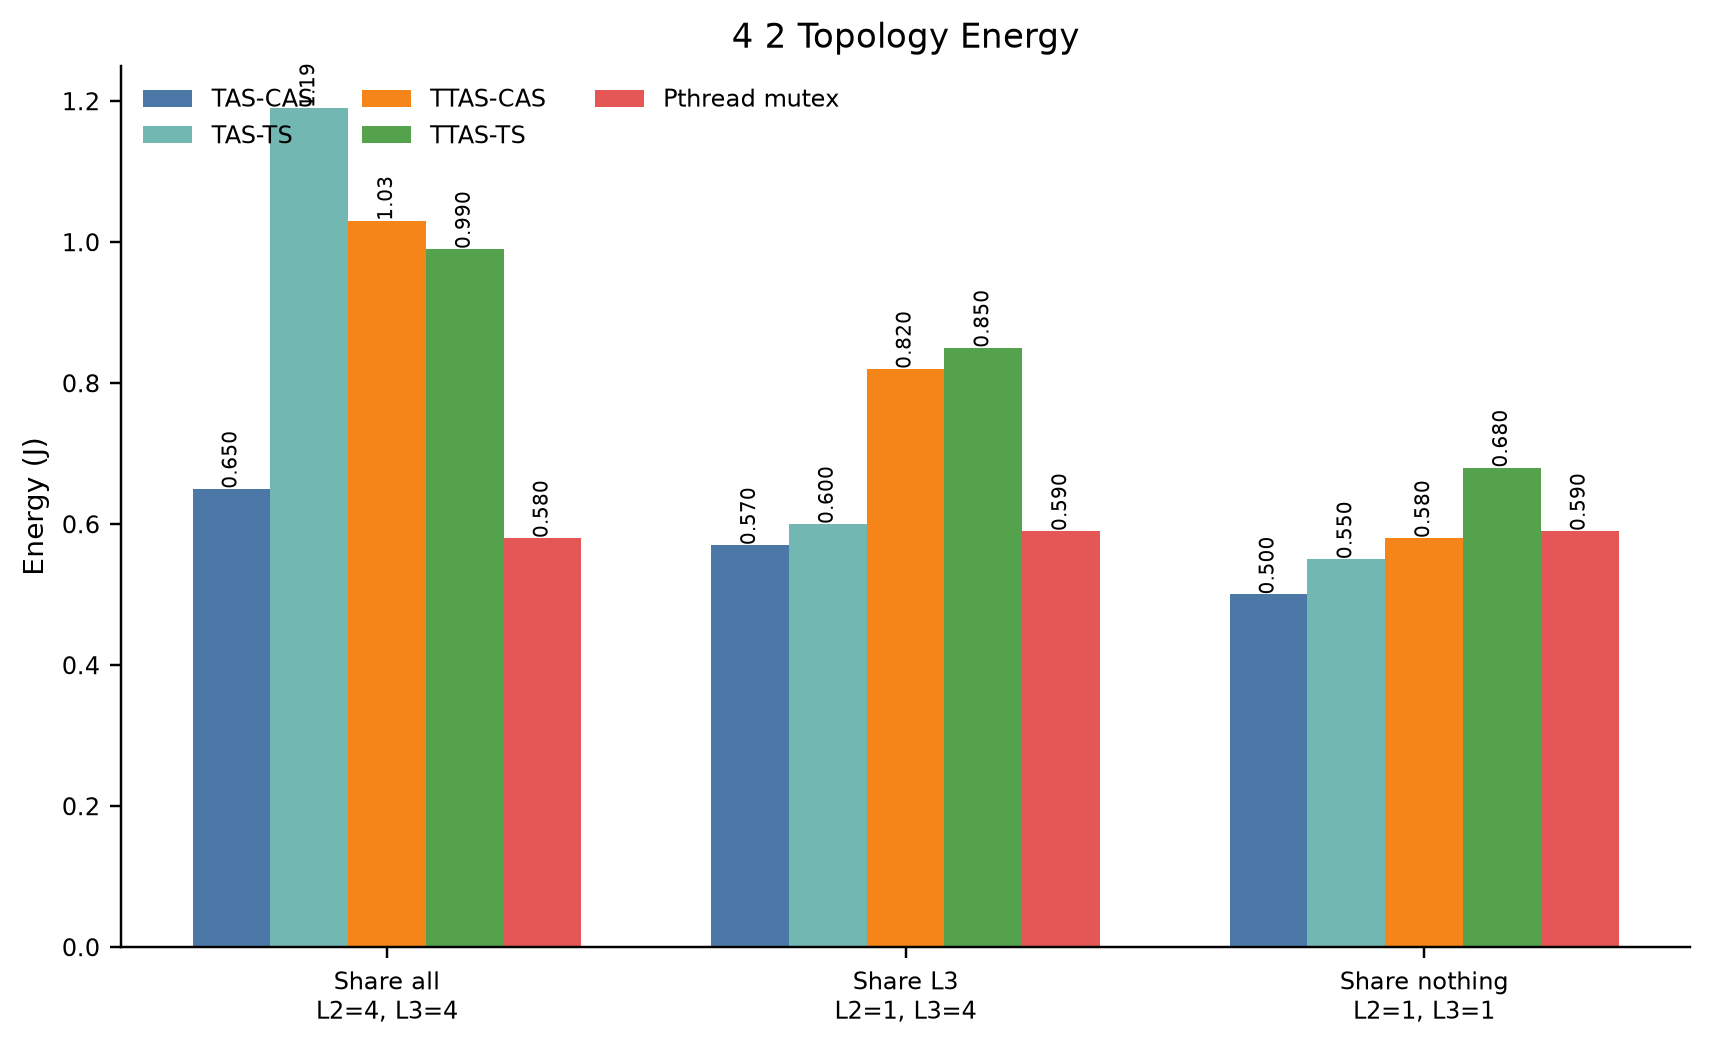
\includegraphics[width=0.82\textwidth]{4_2_topology_energy.png}
\caption{Ενέργεια ανά τοπολογία και υλοποίηση.}
\label{fig:topology-energy}
\end{figure}

Στο Διάγραμμα~\ref{fig:topology-energy}, η \code{TAS_CAS} έχει χαμηλή ενέργεια σε όλες τις τοπολογίες, ειδικά στη \code{share-nothing}, όπου η ενέργεια είναι \(0.50\,\mathrm{J}\). Αντίθετα, η \code{TAS_TS} και οι εκδόσεις TTAS έχουν υψηλότερη ενέργεια στη \code{share-all}, επειδή εκτελούν περισσότερες εντολές ανά μονάδα χρόνου. Η \code{MUTEX} έχει ενέργεια γύρω στα \(0.58\text{--}0.59\,\mathrm{J}\), αλλά αυτό συνοδεύεται από μεγαλύτερο χρόνο εκτέλεσης.

\begin{figure}[htbp]
\centering
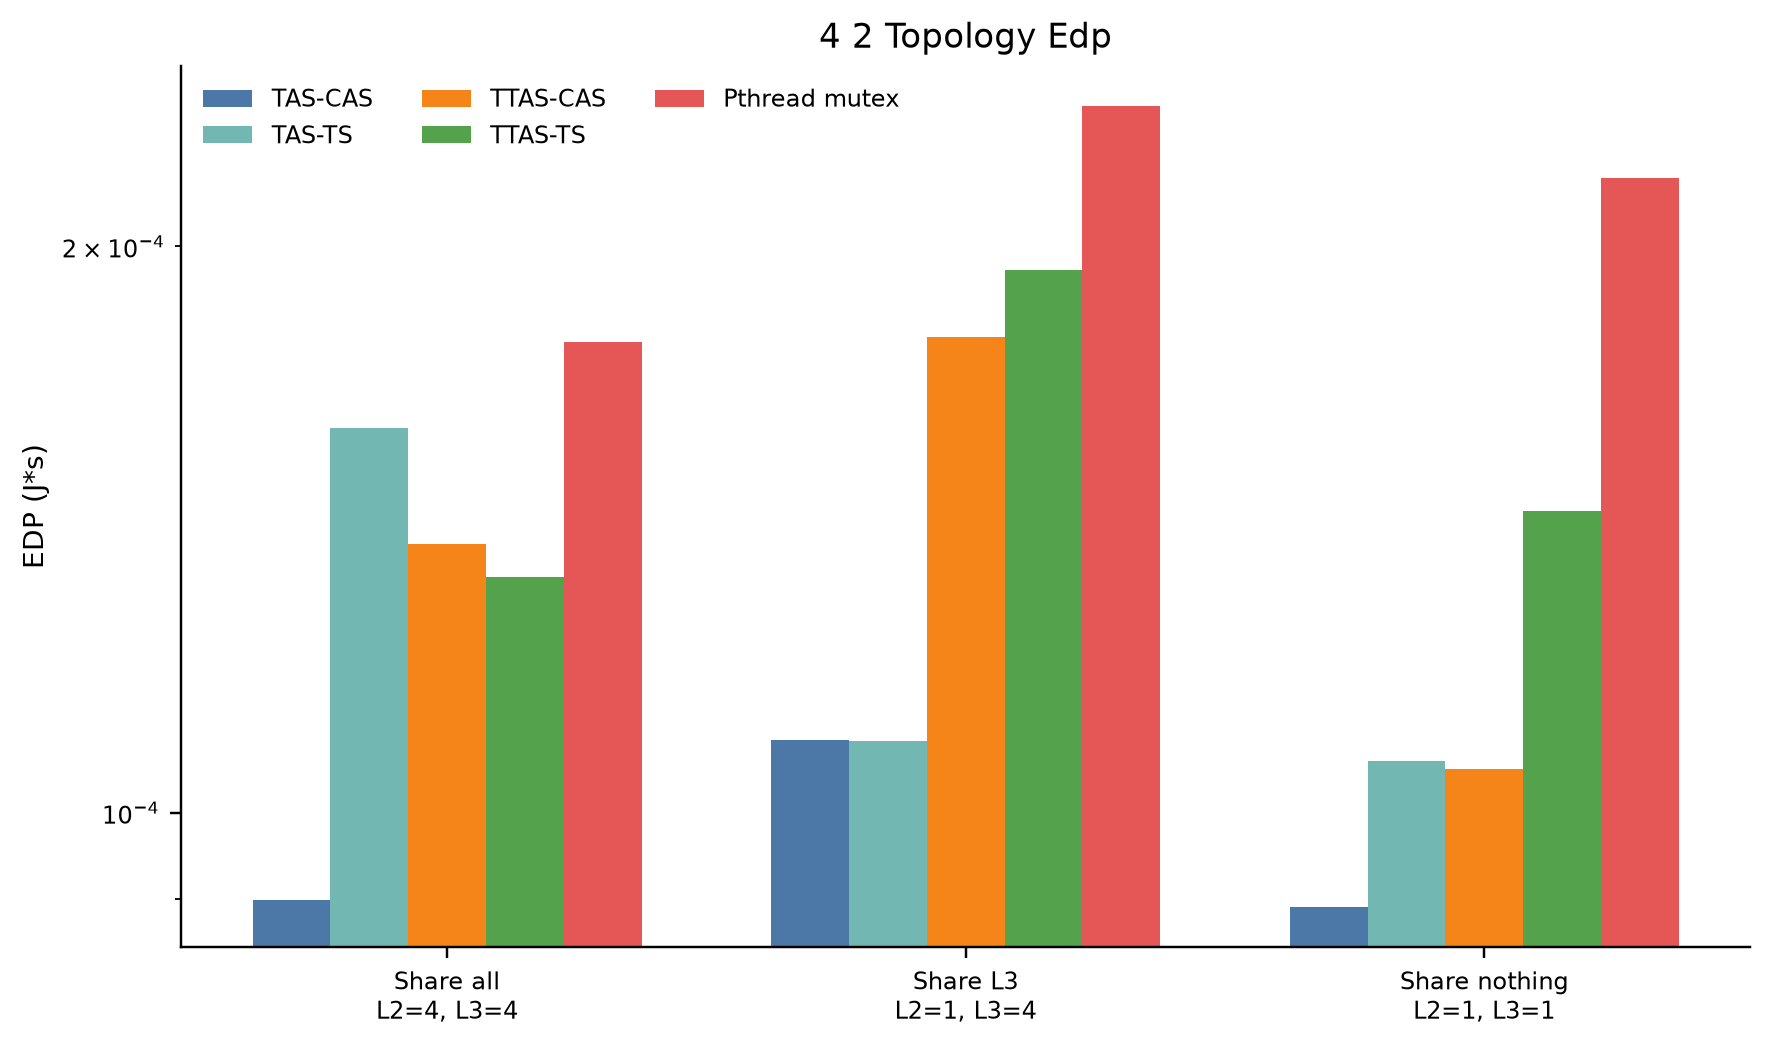
\includegraphics[width=0.82\textwidth]{4_2_topology_edp.png}
\caption{$EDP$ ανά τοπολογία και υλοποίηση.}
\label{fig:topology-edp}
\end{figure}

Το $EDP$ του Διαγράμματος~\ref{fig:topology-edp} δείχνει ότι η \code{TAS_CAS} είναι μία από τις καλύτερες, και σε ορισμένες περιπτώσεις η καλύτερη, επιλογή στις τοπολογίες \code{share-all} και \code{share-nothing}. Στη \code{share-l3}, η \code{TAS_TS} έχει οριακά καλύτερο $EDP$ από την \code{TAS_CAS}. Οι υλοποιήσεις TTAS δεν υπερισχύουν στο $EDP$, επειδή για \code{grain=1} η πρόσθετη εκτέλεση εντολών τους δεν αντισταθμίζεται αρκετά από τη μείωση των ατομικών εγγραφών.

\begin{figure}[htbp]
\centering
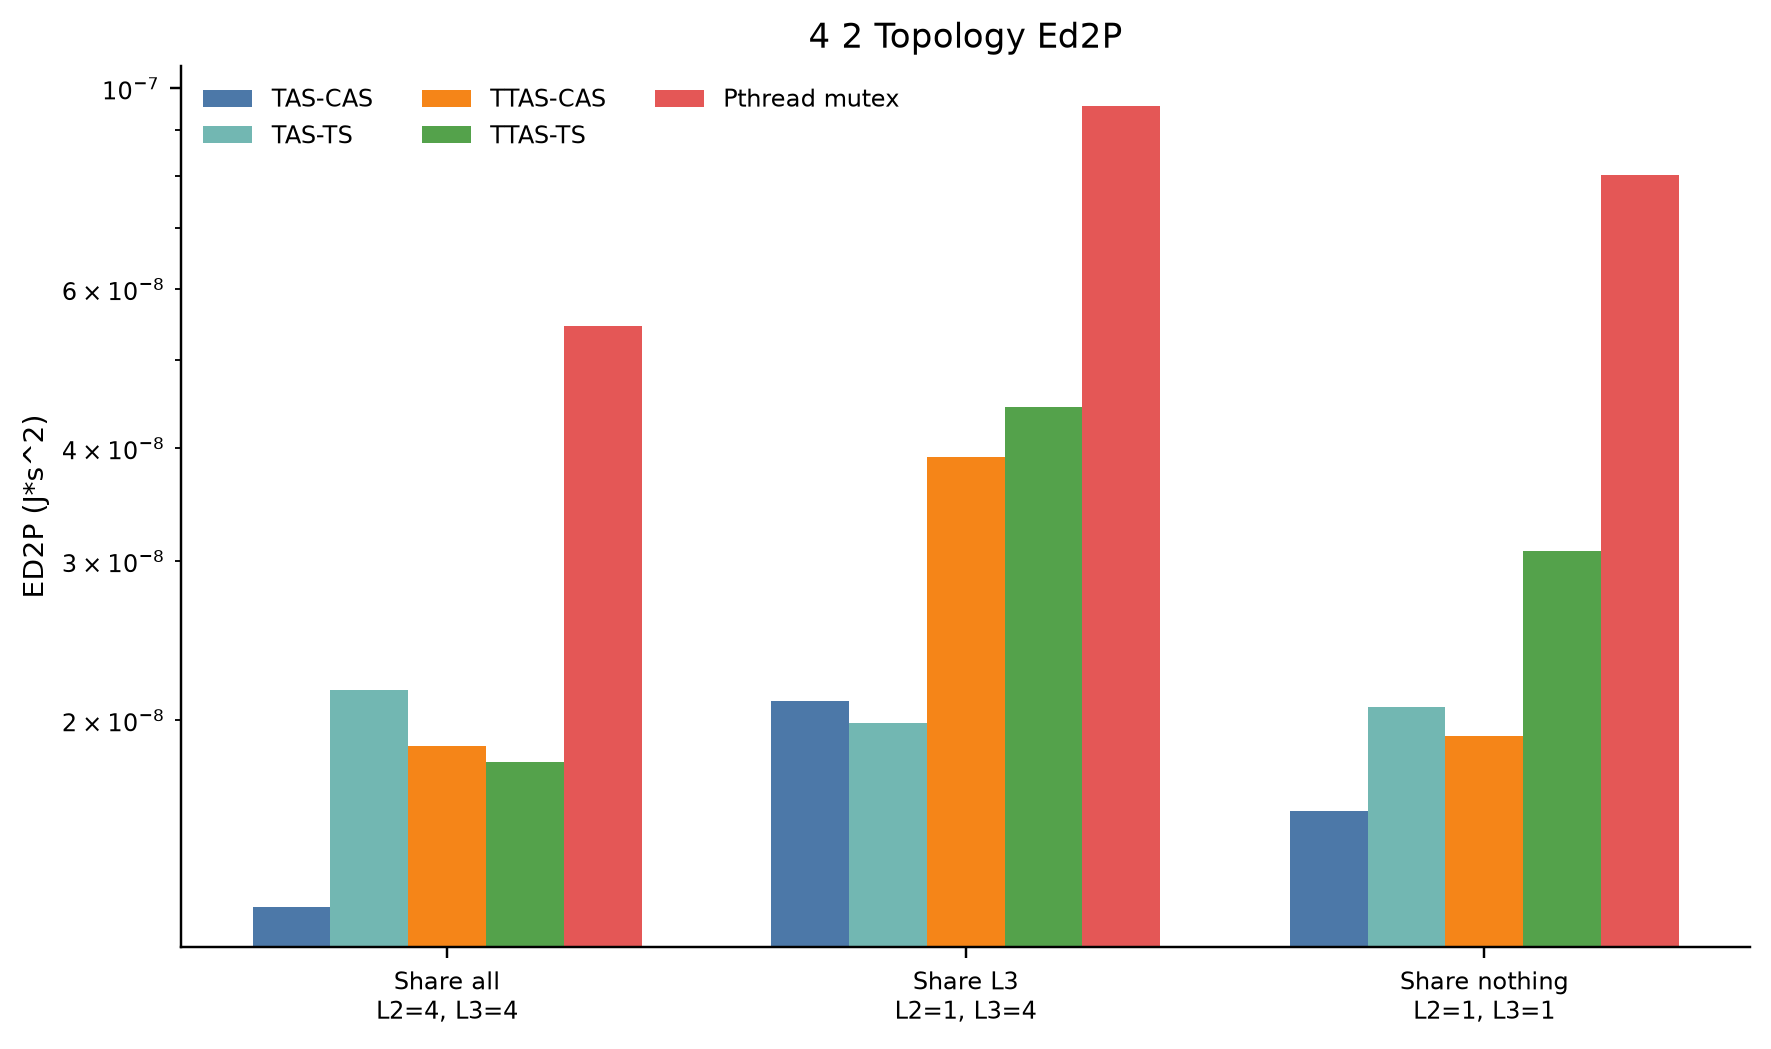
\includegraphics[width=0.82\textwidth]{4_2_topology_ed2p.png}
\caption{$ED^2P$ ανά τοπολογία και υλοποίηση.}
\label{fig:topology-ed2p}
\end{figure}

Το $ED^2P$, που δίνει μεγαλύτερο βάρος στον χρόνο εκτέλεσης, επιβεβαιώνει την ίδια τάση. Οι εκδόσεις TAS παραμένουν πιο ισορροπημένες για αυτή τη μικρή κρίσιμη περιοχή, ενώ το \code{MUTEX} επιβαρύνεται λόγω υψηλότερου χρόνου εκτέλεσης.

\subsection{Συνδυασμένη εικόνα χρόνου, ενέργειας και $EDP$}

\begin{figure}[htbp]
\centering
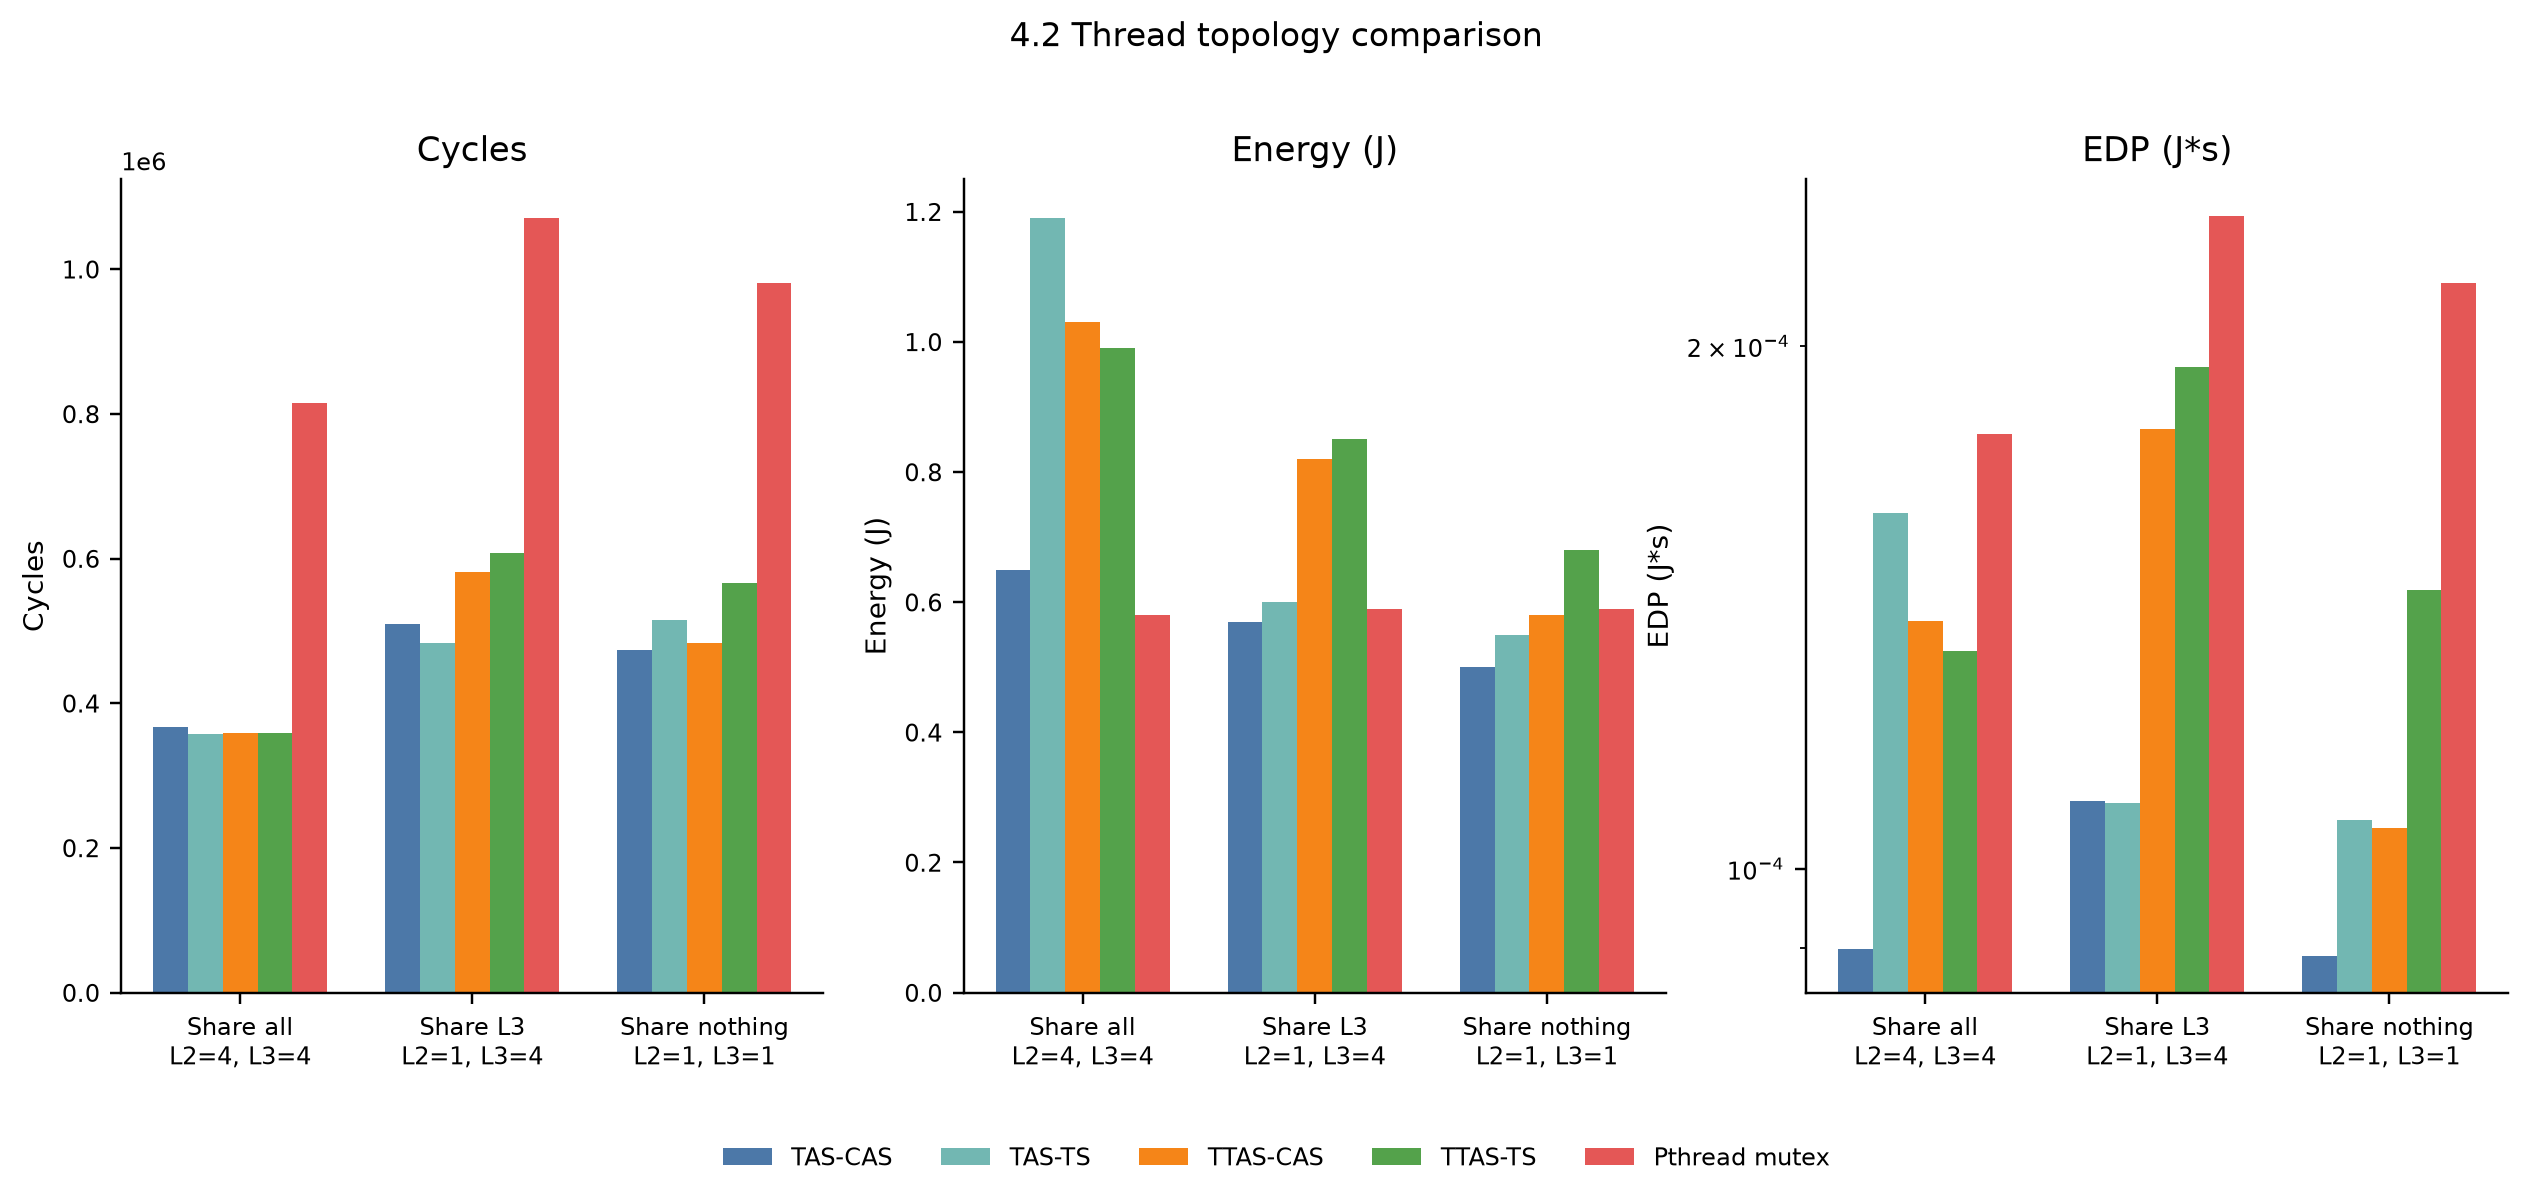
\includegraphics[width=0.86\textwidth]{4_2_topology_runtime_energy_edp.png}
\caption{Συνδυασμένη παρουσίαση χρόνου, ενέργειας και $EDP$ στα πειράματα τοπολογίας.}
\label{fig:topology-runtime-energy-edp}
\end{figure}

Το Διάγραμμα~\ref{fig:topology-runtime-energy-edp} συνοψίζει τη βασική παρατήρηση των πειραμάτων τοπολογίας. Για πολύ μικρή κρίσιμη περιοχή, η απλότητα του path του lock είναι κρίσιμη. Οι υλοποιήσεις TAS, ειδικά η \code{TAS_CAS}, δίνουν συχνά καλύτερη συνολική ισορροπία. Οι υλοποιήσεις TTAS μειώνουν θεωρητικά το coherence traffic, αλλά σε τόσο μικρή κρίσιμη περιοχή η επιπλέον διαδικασία polling δεν αποδίδει αρκετά. Η τοπολογία επηρεάζει τα αποτελέσματα, αλλά δεν αλλάζει πλήρως την κατάταξη των μηχανισμών.

\subsection{Πλήρη αριθμητικά αποτελέσματα τοπολογίας}

\begin{table}[htbp]
\centering
\scriptsize
\caption{Πλήρη αριθμητικά αποτελέσματα πειραμάτων τοπολογίας.}
\label{tab:topology-full-results}
\resizebox{\textwidth}{!}{
\begin{tabular}{P{2.8cm} P{2.3cm} P{1.3cm} P{1.3cm} P{2.1cm} P{2.1cm} P{1.8cm} P{1.8cm} P{1.8cm} P{2.0cm} P{2.2cm}}
\toprule
\textbf{Τοπολογία} & \textbf{Υλοποίηση} & \textbf{L2} & \textbf{L3} & \textbf{Instr.} & \textbf{Cycles} & \textbf{Runtime (s)} & \textbf{Power (W)} & \textbf{Energy (J)} & \textbf{EDP (J s)} & \textbf{ED$^2$P (J s$^2$)} \\
\midrule
\code{share-all} & \code{MUTEX} & 4 & 4 & 350185 & 815648 & 0.000306635 & 1880.28 & 0.58 & 0.000177848 & 5.4535e-08 \\
\code{share-all} & \code{TAS_CAS} & 4 & 4 & 417092 & 367708 & 0.000138236 & 4674.32 & 0.65 & 8.98534e-05 & 1.2421e-08 \\
\code{share-all} & \code{TAS_TS} & 4 & 4 & 809984 & 358067 & 0.000134612 & 8875.00 & 1.19 & 0.000160188 & 2.1563e-08 \\
\code{share-all} & \code{TTAS_CAS} & 4 & 4 & 778174 & 358615 & 0.000134818 & 7648.13 & 1.03 & 0.000138863 & 1.8721e-08 \\
\code{share-all} & \code{TTAS_TS} & 4 & 4 & 746026 & 358434 & 0.000134750 & 7322.72 & 0.99 & 0.000133403 & 1.7976e-08 \\
\midrule
\code{share-l3} & \code{MUTEX} & 1 & 4 & 346385 & 1070543 & 0.000402460 & 1465.02 & 0.59 & 0.000237451 & 9.5565e-08 \\
\code{share-l3} & \code{TAS_CAS} & 1 & 4 & 362134 & 510158 & 0.000191789 & 2956.51 & 0.57 & 0.000109320 & 2.0966e-08 \\
\code{share-l3} & \code{TAS_TS} & 1 & 4 & 397950 & 483855 & 0.000181901 & 3296.37 & 0.60 & 0.000109141 & 1.9853e-08 \\
\code{share-l3} & \code{TTAS_CAS} & 1 & 4 & 593000 & 580885 & 0.000218378 & 3750.98 & 0.82 & 0.000179070 & 3.9105e-08 \\
\code{share-l3} & \code{TTAS_TS} & 1 & 4 & 623055 & 608246 & 0.000228664 & 3730.11 & 0.85 & 0.000194364 & 4.4444e-08 \\
\midrule
\code{share-nothing} & \code{MUTEX} & 1 & 1 & 350225 & 980267 & 0.000368522 & 1611.52 & 0.59 & 0.000217428 & 8.0127e-08 \\
\code{share-nothing} & \code{TAS_CAS} & 1 & 1 & 318671 & 473997 & 0.000178195 & 2785.63 & 0.50 & 8.90975e-05 & 1.5877e-08 \\
\code{share-nothing} & \code{TAS_TS} & 1 & 1 & 358372 & 515471 & 0.000193786 & 2819.52 & 0.55 & 0.000106582 & 2.0654e-08 \\
\code{share-nothing} & \code{TTAS_CAS} & 1 & 1 & 404321 & 483674 & 0.000181833 & 3210.80 & 0.58 & 0.000105463 & 1.9177e-08 \\
\code{share-nothing} & \code{TTAS_TS} & 1 & 1 & 479024 & 565954 & 0.000212765 & 3179.05 & 0.68 & 0.000144680 & 3.0783e-08 \\
\bottomrule
\end{tabular}
}
\end{table}

\FloatBarrier

\section{Συζήτηση}

\subsection{Σύνδεση με τη θεωρία του μαθήματος}

Τα αποτελέσματα της εργασίας συνδέονται άμεσα με τρεις βασικές θεματικές του μαθήματος: τον παραλληλισμό επιπέδου νήματος, τη συνάφεια κρυφών μνημών και τη συνέπεια μνήμης.

Αρχικά, το benchmark εκφράζει TLP μέσω Pthreads. Ωστόσο, η ύπαρξη μίας κοινής κρίσιμης περιοχής περιορίζει τον πραγματικό παραλληλισμό. Η αύξηση των νημάτων δεν σημαίνει αυτόματα επιτάχυνση, επειδή τα νήματα πρέπει να σειριοποιηθούν γύρω από το lock. Αυτό αποτελεί πρακτική εφαρμογή της γενικής αρχής ότι η απόδοση ενός παράλληλου προγράμματος περιορίζεται από το σειριακό του τμήμα και από το κόστος επικοινωνίας/συγχρονισμού.

Δεύτερον, τα locks είναι ιδιαίτερα ευαίσθητα στο cache coherence. Η μεταβλητή lock βρίσκεται σε μία cache line που προσπελαύνεται από όλους τους πυρήνες. Στις υλοποιήσεις TAS, κάθε αποτυχημένη προσπάθεια απόκτησης είναι ατομική read-modify-write πράξη, άρα δημιουργεί συνεχείς απαιτήσεις για αποκλειστική πρόσβαση στη cache line. Αυτό επιβαρύνει το coherence protocol. Στις υλοποιήσεις TTAS, η αναμονή γίνεται κυρίως με απλές αναγνώσεις, οπότε η cache line μπορεί να παραμένει σε κατάσταση shared μέχρι να φανεί ότι το lock είναι ελεύθερο. Αυτή είναι η βασική αρχιτεκτονική διαφορά μεταξύ TAS και TTAS.

Τρίτον, η ορθότητα των locks προϋποθέτει κατάλληλες εγγυήσεις διάταξης μνήμης. Το release του lock πρέπει να γίνεται αφού οι εγγραφές της κρίσιμης περιοχής έχουν γίνει ορατές με τη σωστή σειρά. Διαφορετικά, ένα άλλο νήμα θα μπορούσε να αποκτήσει το lock και να δει ασυνεπή κατάσταση. Η χρήση των atomic intrinsics της GCC και του \code{pthread_mutex} παρέχει την απαραίτητη σημασιολογία διάταξης μνήμης για τη συγκεκριμένη υλοποίηση.

\subsection{Γιατί διαφέρουν Sniper και πραγματικό σύστημα}

Η απόκλιση μεταξύ Sniper και πραγματικού συστήματος είναι αναμενόμενη και χρήσιμη. Ο Sniper επιτρέπει ελεγχόμενη αρχιτεκτονική διερεύνηση, αλλά δεν αναπαράγει πλήρως όλα τα χαρακτηριστικά ενός σύγχρονου laptop CPU. Το πραγματικό σύστημα διαθέτει υβριδική τοπολογία, SMT σε μέρος των πυρήνων, δυναμική συχνότητα και πραγματικό λειτουργικό σύστημα. Επιπλέον, το mutex της Pthreads στο πραγματικό σύστημα είναι υλοποίηση συστήματος με βελτιστοποιήσεις που δεν ισοδυναμούν με ένα απλό spinlock.

Στον Sniper, τα spinlocks είναι συχνά ταχύτερα σε κύκλους από το \code{MUTEX}, επειδή αποφεύγουν το overhead της βιβλιοθήκης και του path συγχρονισμού του mutex. Στο πραγματικό σύστημα, όμως, το ενεργό spinning μπορεί να γίνει ιδιαίτερα επιβαρυντικό για μικρή τιμή grain και πολλά νήματα. Εκεί το mutex υπερισχύει επειδή μειώνει την ενεργή κατανάλωση πόρων CPU κατά την αναμονή.

Στις μεγαλύτερες τιμές grain, και τα δύο περιβάλλοντα δείχνουν ότι οι υλοποιήσεις TTAS είναι πιο κατάλληλες ως προς τον χρόνο εκτέλεσης σε συνθήκες contention. Η ποιοτική τάση, δηλαδή ότι το TTAS βοηθά όταν η αναμονή είναι αρκετά μεγάλη, επιβεβαιώνεται και στα δύο περιβάλλοντα.

\subsection{Επίδραση του grain}

Η παράμετρος \code{grain} είναι κρίσιμη, επειδή καθορίζει τη σχέση μεταξύ χρήσιμης εργασίας και κόστους συγχρονισμού.

Για \code{grain=1}, το benchmark μετρά σχεδόν καθαρά το κόστος lock/unlock. Εκεί η απλότητα του TAS μπορεί να είναι πλεονέκτημα στον Sniper, ενώ στο πραγματικό σύστημα το mutex αποφεύγει την υπερβολική ενεργό αναμονή σε πολλά νήματα.

Για \code{grain=10}, αρχίζει να εμφανίζεται ισορροπία. Οι υλοποιήσεις TTAS μπορούν να μειώσουν το coherence traffic χωρίς να επιβαρύνουν δυσανάλογα την εκτέλεση. Στο πραγματικό σύστημα η \code{TTAS_TS} και η \code{TTAS_CAS} είναι συχνά οι καλύτερες.

Για \code{grain=100}, το TTAS υπερισχύει καθαρά ως προς τον χρόνο εκτέλεσης, επειδή οι αποτυχημένες ατομικές προσπάθειες των locks TAS γίνονται ιδιαίτερα ακριβές όταν πολλοί πυρήνες περιμένουν για περισσότερο χρόνο. Ωστόσο, στον Sniper η ενεργειακή ανάλυση δείχνει ότι αυτό δεν είναι απαραίτητα ενεργειακά βέλτιστο.

\subsection{Επίδραση τοπολογίας}

Τα πειράματα τοπολογίας δείχνουν ότι η θέση των νημάτων στην ιεραρχία της cache επηρεάζει την απόδοση. Όταν τα νήματα μοιράζονται L2 και L3, η επικοινωνία για τη cache line του lock γίνεται πιο κοντά στους πυρήνες και οι υλοποιήσεις spinlock έχουν καλύτερη συμπεριφορά. Όταν η κοινή cache βρίσκεται πιο μακριά ή δεν υπάρχει κοινό επίπεδο μεταξύ των πυρήνων, το κόστος coherence αυξάνεται.

Παρ' όλα αυτά, η τοπολογία δεν αλλάζει πλήρως τη βασική κατάταξη. Για \code{grain=1}, οι εκδόσεις TAS παραμένουν πολύ ανταγωνιστικές επειδή έχουν μικρότερο επιπλέον κόστος εντολών. Οι εκδόσεις TTAS χρειάζονται μεγαλύτερο χρόνο αναμονής για να φανεί το πλεονέκτημά τους.

\section{Συμπεράσματα}

Στην εργασία αυτή υλοποιήθηκαν και αξιολογήθηκαν πέντε μηχανισμοί συγχρονισμού: \code{TAS_CAS}, \code{TAS_TS}, \code{TTAS_CAS}, \code{TTAS_TS} και \code{MUTEX}. Όλες οι υλοποιήσεις ολοκλήρωσαν επιτυχώς τα πειράματα και πέρασαν τον έλεγχο ορθότητας, δηλαδή η τελική τιμή της διαμοιραζόμενης μεταβλητής ήταν ίση με $\text{\texttt{nthreads}} \cdot \text{\texttt{iterations}}$.

Τα αποτελέσματα δείχνουν ότι δεν υπάρχει καθολικά βέλτιστος μηχανισμός συγχρονισμού. Η καλύτερη επιλογή εξαρτάται από το μέγεθος της κρίσιμης περιοχής, τον αριθμό των νημάτων, την τοπολογία της ιεραρχίας της cache και το αν ο στόχος είναι ο ελάχιστος χρόνος ή η καλύτερη ενεργειακή αποδοτικότητα.

Στον Sniper, οι υλοποιήσεις TAS είναι ιδιαίτερα ανταγωνιστικές για μικρή τιμή grain, ενώ οι υλοποιήσεις TTAS γίνονται καλύτερες σε κύκλους για μεγαλύτερη τιμή grain και υψηλότερο contention. Ωστόσο, η ενεργειακή ανάλυση μέσω McPAT δείχνει ότι οι υλοποιήσεις TTAS μπορούν να έχουν πολύ μεγάλο ενεργειακό κόστος, λόγω του μεγάλου πλήθους εντολών που εκτελούνται κατά το polling. Επομένως, η βελτίωση στον χρόνο δεν συνεπάγεται απαραίτητα βελτίωση στο $EDP$ ή στο $ED^2P$.

Στο πραγματικό σύστημα, το mutex της Pthreads είναι η καλύτερη επιλογή για \code{grain=1} και πολλά νήματα, επειδή αποφεύγει την υπερβολική ενεργό αναμονή των spinlocks. Για \code{grain=10} και \code{grain=100}, οι υλοποιήσεις TTAS υπερισχύουν συχνά, επιβεβαιώνοντας ότι η συμπεριφορά spin-on-read βοηθά όταν η αναμονή για το lock είναι αρκετά μεγάλη.

Τα πειράματα τοπολογίας δείχνουν ότι ο διαμοιρασμός cache επηρεάζει σημαντικά το κόστος συγχρονισμού. Η \code{share-all} τοπολογία είναι γενικά πιο ευνοϊκή για τα spinlocks, ενώ όταν οι πυρήνες δεν μοιράζονται χαμηλά επίπεδα cache, η μεταφορά της cache line του lock γίνεται ακριβότερη. Παρ' όλα αυτά, για μικρή κρίσιμη περιοχή το κόστος του ίδιου του path του lock παραμένει εξίσου καθοριστικό με την τοπολογία.

Συνολικά, η εργασία επιβεβαιώνει ότι οι μηχανισμοί συγχρονισμού δεν μπορούν να αξιολογηθούν ανεξάρτητα από την αρχιτεκτονική. Ένα lock είναι ταυτόχρονα προγραμματιστική δομή και αρχιτεκτονικό φορτίο εργασίας για το coherence protocol. Οι ατομικές εντολές, η ιεραρχία της cache, το μοντέλο συνέπειας μνήμης, η τοπολογία πυρήνων και η πολιτική του runtime επηρεάζουν άμεσα την τελική απόδοση. Γι' αυτό, σε πραγματικά πολυπύρηνα συστήματα, η επιλογή μηχανισμού συγχρονισμού πρέπει να γίνεται με βάση το είδος του φορτίου εργασίας και όχι μόνο με βάση τη θεωρητική απλότητα της υλοποίησης.

\end{document}
